%%%%%%%%%%%%%%%%%%%%%%%%%%%%%%%%%%%%%
% To-do
%%%%%%%%%%%%%%%%%%%%%%%%%%%%%%%%%%%%%
% - El primer parrafo no tiene identacion, solucionar.
% - ¿Donde cuentas que necesitas?
% - ¿Tienes que decir todo lo que hay en los ficheros de configuración?

%%%%%%%%%%%%%%%%%%%%%%%%%%%%%%%%%%%%%
% Final report
%%%%%%%%%%%%%%%%%%%%%%%%%%%%%%%%%%%%%
\documentclass{article}

% libraries
%%%%%%%%%%%%%%%%%%%%%%%%%%%%%%%%%%%%%
\usepackage[utf8]{inputenc}
\usepackage{geometry}
\usepackage{float}
\usepackage{amsmath}
\usepackage{url}
\usepackage{fancyhdr}
\usepackage{graphicx}
\usepackage{setspace}
\usepackage{listings}
\usepackage[numbered,autolinebreaks,useliterate]{mcode}
\usepackage{pdfpages}
\usepackage{booktabs}
\usepackage{bigstrut}
\usepackage{bigdelim}
\usepackage{multirow}
\usepackage[nottoc]{tocbibind}
\usepackage{rotating} 
\usepackage[parfill]{parskip}
\usepackage{tabu}
\usepackage{setspace}
\usepackage{hyperref}
\usepackage{caption}
\usepackage{wrapfig}
\usepackage{natbib}
\usepackage{array}
\usepackage{makecell}

% Setting links
%%%%%%%%%%%%%%%%%%%%%%%%%%%%%%%%%%%%%
\hypersetup{
	colorlinks,
	citecolor=black,
	filecolor=black,
	linkcolor=black,
	urlcolor=black
}

\DeclareCaptionLabelFormat{andtable}{#1~#2  \&  \tablename~\thetable}

% Page style
%%%%%%%%%%%%%%%%%%%%%%%%%%%%%%%%%%%%%
\geometry{paper=a4paper, left=25mm, right=25mm, top=30mm, bottom=30mm, headsep=10mm}
\pagestyle{fancy}
\fancyhf{}
\setlength{\parindent}{12pt}

% Header and Footer
%%%%%%%%%%%%%%%%%%%%%%%%%%%%%%%%%%%%%
\fancyhead[L]{Final report}
\fancyhead[R]{Samuel Góngora García}
\fancyfoot[C]{\thepage}  % Change to something prettier

\renewcommand{\headrulewidth}{0.5 pt}

% Now we start the main document body
%%%%%%%%%%%%%%%%%%%%%%%%%%%%%%%%%%%%%
\begin{document}
\begin{titlepage}
\centering
\includegraphics[width=0.15\textwidth]{example-image-1x1}\par\vspace{1cm}
{\scshape\LARGE Columbidae University \par}
\vspace{1cm}
{\scshape\Large Final year project\par}
\vspace{1.5cm}
{\huge\bfseries Pigeons love doves\par}
\vspace{2cm}
{\Large\itshape Samuel Góngora García\par}
\vfill
supervised by\par
Dr.~Mark \textsc{Brown}

\vfill
% Bottom of the page
{\large \today\par}
\end{titlepage}
\newpage\null\thispagestyle{empty}\newpage
% Abstract
%%%%%%%%%%%%%%%%%%%%%%%%%%%%%%%%%%%%%
\begin{abstract}
This report covers the development process of an application intended to analyze the Euclid future data. An opportunity to use the incoming images in a totally different way was seen.
\end{abstract}
\newpage\null\newpage

% Table of Contents
%%%%%%%%%%%%%%%%%%%%%%%%%%%%%%%%%%%%%
\newpage	
% Create the table of contents.
\begin{center}
\renewcommand\contentsname{\LARGE{\underline{Index}}}
\tableofcontents
\end{center}
\newpage\null\newpage

% Create the table of figures.
\begin{center}
\renewcommand\contentsname{\LARGE{\underline{Figures}}}
\listoffigures
\end{center}
\newpage\null\newpage

% Create the table of tables.
\begin{center}
\renewcommand\contentsname{\LARGE{\underline{Tables}}}
\listoftables
\end{center}
\newpage\null\newpage

% Sections and Subsections
%%%%%%%%%%%%%%%%%%%%%%%%%%%%%%%%%%%%%
% Introduction paragraph
\section{Introduction}
Euclid mission is going to produce a huge amount of high quality astronomical images. These images can be use to discover new objects, in our particular case, solar system minor bodies. An important fact related to this mission is that the survey is going to cover a very low objects number population Solar System areas. The number of new bodies to be discovered was deeply discussed by BENOIT CARRY in several studies.
\par
The purpose of this Report is to summarize the research process of the best set-up possible to detect minor bodies across the telescope images. Because the usage of mocked data these values could be not the best in a future real situation. Anyway, steps taken for this study can be reproduced again with a different images, in order to get the new configuration values for the new data.

\subsection{Report structure}
Firstly a quick view over the existing software will be taken. This will give us an idea about which utilities can be exploited for our purposes. Then a explanation about the nature of data will be made. The type of the files which will received, the internal organization of them and the capabilities of the CCD sensors.
\par Taking account of the incoming data and our targets an analysis of the best configuration available for the existing software will be performed. Once we have the raw data a filtering process will be run on them. The different techniques applied are going to be discussed and tested.
\par In the end the pros and cons of the created pipeline will be reviewed. A few ideas about future improvements will be exposed.

\subsection{Acknowledgements}
This project was created in blablalba gracias a blablaba. Gracias a blabla por su apoyo y blabla.

\section{Initial software}
For the extraction operation two different programs are going to be used. These utilities have been chosen because they are well maintained by his creator and have been proven over years of use. The main objective of this study is to code a pipeline using Python which will be in charge to called those utilities whenever will be necessary.
\par Beside this, the pipeline should be capable of adapt his behaviour to fit in any environment. It must make use of all hardware capabilities in order to run the pipeline as fast as possible.

\subsection{SExtractor}
Created by Emmanuel Bertin SEXtractor\footnote{\url{https://www.astromatic.net/software/sextractor}} (from Source Extractor) is a program that builds a catalogue of objects from astronomical images. Originally designed for galaxy extraction this software can be tuned in order to work with minor planets. In order to make any change in SExtractor behaviour this software has some configuration files that can be modify.
\par Relevant parameters in SExtractor configuration files are going to be discussed in this Report.

\subsection{SCAMP}
Also coded by Emmanuel Bertin SCAMP\footnote{\url{https://www.astromatic.net/software/scamp}} is an utility designed to reads SExtractor catalogs and computes astrometric and photometric solutions. This software can take as a input catalogs from any time and position. Like SExtractor was also created to deal with galaxies, but it can be tune in order to work with minor planet bodies.

\subsection{Python}
This programming language was chosen due to the ease of scripts creation. In addition, any software created using Python in a particular operating system can be easily move to another one.
\par By now Python has two major versions, 2.x and 3.x. Although 2.x version still has a great support of the community in a near future it will become obsolete. The whole pipeline will be create to be run as a Python 3.x executable.
\par The Python necessary modules for software utilization will be installed through an installation script.

\section{Input data}
In this section we are going to introduce which kind of image will our pipeline receive and the distribution of motion and magnitude of the expected minor bodies. Software configuration will be chosen to maximize the performance at those values.

\subsection{Sensor}
For this study we are going to use the VIS camera of Euclid spacecraft. This camera is composed by thirty-six CCD devices disposed in a matrix of six rows per six columns. Each CCD itself is formed by four quadrants of the same size counting a total of 4096 per 4132 pixels with a pixel size of twelve micron.
\par The VIS focal plane covers a field of view of 0.57 square degrees with 0.1 arc-second pixels. VIS will be equipped with one single very broad band filter covering the wavelength range from 550 nm to 900 mn with a mean image quality of about 0.23 arc-second.\footnote{\url{https://www.euclid-ec.org/?page_id=2485}}

\subsection{Images type}
All the quadrants are save in the same file. Each file have one hundred and forty-four images. For each CCD the lower-left quadrant will be always the first of the while the upper-right is the last in the sequence of four. The software is in charge to merge properly the quadrants taking account of overlap areas.
\par While in the final data there will be flat field images and glitches maps in this study they are not going to be take in account.
% Figure creation
\begin{figure}[H]
\centering
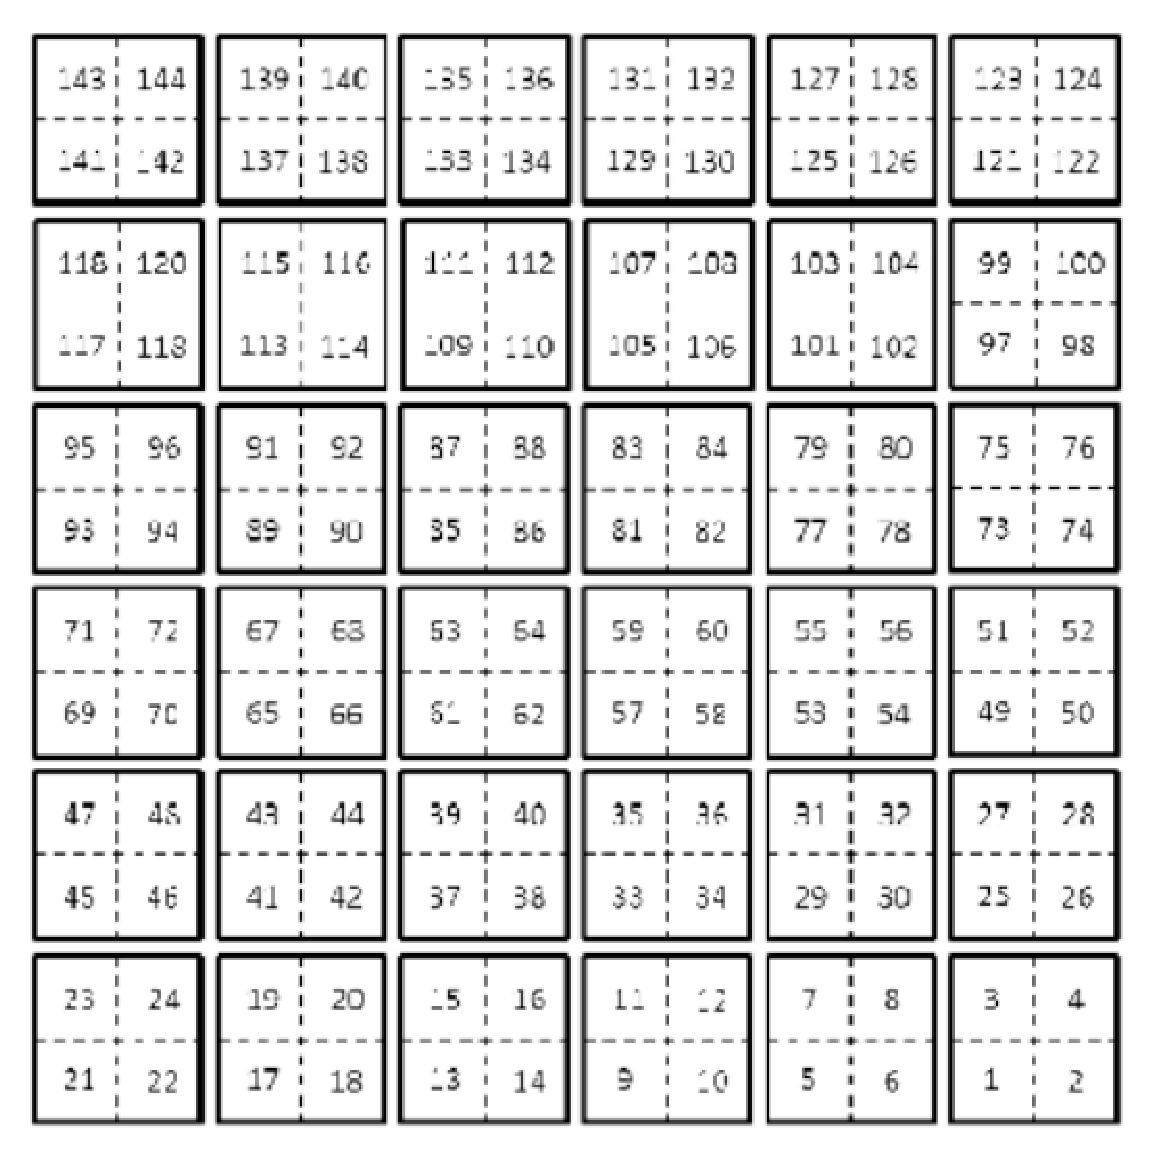
\includegraphics[width=.5\linewidth]{images/quadrants_order.eps}
\caption{Quadrants order inside FPA image file}
\end{figure}

\subsection{Solar system objects proper motions and magnitudes}
Objective magnitudes of Euclid Survey are going to be between 21-27. Gaia va a estar mirando a magnitudes inferiores asi que no se descubrirá nada nuevo

\section{Sextractor analysis}
Search for the best configuration parameters for SExtractor process seems to be the first step in the development of a full pipeline for solar system objects extraction.
In this paper we are going to take a look over the entire analysis process which brings us the best parameters for our particular images configuration.

% Images description
\subsection{Images simulated}
For the SEXtractor analysis three images were simulated. Each one covering a different range of magnitudes. Each single pair of speed and proper motion combination has one hundred of objects.
\par
No stars or galaxies are simulated in these images. To speed up the extraction process cosmic rays and another glitches were left out of images.

\subsection{SSOs nature and disposition}
In order to simplify extraction process objects are disposed on a regular matrix. 
This matrix contains blabla rows and blabla columns. TODO
\par
% Define objects position
From 0 to objects magnitude decreasing values. X-axis.
Y-axis speeds. TODO

\subsubsection{Input catalogs}
Three different catalogs, \textit{(1\_CatNoStars\_24-25.dat, 2\_CatNoStars\_25-26.dat and 1\_CatNoStars\_26-27.dat)} were created as starting points for images creation. 
These catalogs can be read as a comma separated value file where each column represents a different parameter.
\par
First and second column give us x and y position in final image. These positions are expressed in pixel units. As fits file has WCS information right ascension and declination values can be easily obtained.
\par
Third column shows magnitude. 
\par
Forth column values are the proper motions of objects meanwhile last column shows proper angles associated to those motions.

% Analytical approach 
\subsection{Analysis approach}
Our analysis will be focused on the faintest and slowest objects. A completely different approach, using another algorithm, will be used for faster objects.
\par
A single analysis of each possible magnitude cannot be achieved in this kind of approach. Magnitudes were split in three main groups. 24 to 25, 25 to 26 and 26 to 27.
\par
In the same way five representative proper motions were chosen. Those speeds will cover from the slowest objects available to objects with which sextractor starts to have problems extraction them as single sources. Speeds chosen were 0.001, 1, 3, 5, and 10. All of them expressed as arcseconds per hour.

% Configuration set-up
\subsubsection{Configuration input}
For all configuration variables associated with sextractor configuration file only four elements are important for our study.
\begin{itemize}
\item deblending number: trying to avoid multiple detections in a single object deblending number was set at a high value, this is, 0.1.
\item analysis/detection threshold: different threshold values will give us a clearly different output. That parameter is the key of this analysis, a range of values between 1.2 and 2 were chosen. 
\item detection minimum area: a high value won't detect small objects, this setting was set at four.
\item filter: filter election plays an important role in extraction process. For this particular scenario we chose two different filters: \textit{gauss\_2.0\_5x5 and tophat\_2.0\_3x3}.
\end{itemize}

% Rightful extractions versus total extractions
\subsubsection{True extractions vs. total extractions}
True extractions against total extractions can gave us a better comprehension of filter behavior.
\par
A true extraction is understood as a extraction made by sextractor in the center of the trail of the object. Any other measured made in another location is listed as a false extraction.

% Purity versus completeness
\subsubsection{Purity factor vs. completeness factor}
Performance was measured as a relation between purity factor and completeness factor. These two factors are obtained from the number of true and false sources extracted.
\begin{itemize}
\item Purity factor is the ratio of the number of true sources extracted to the total number of sources extracted. By definition this value cannot exceed 1.0. 
\item Completeness factor is the ratio of the number of true sources extracted related to the number of input sources which is, in our study, a hundred. 
\end{itemize}

% Output
\subsection{Output format}
As we said data is stored in a single file called \textit{full\_stats.csv}. Although each single solution can be found in this file the format chosen is not easily readable.
\par
A series of figures were created plotting purity factor against completeness factor and rightful detections against total ones. Each one showing an unique combination of proper motion and magnitude.
\par
To have a clearer view of solutions each filter each one has a different color and a different marker. Data related to gauss filter is painted in green color meanwhile data created using tophat filter is show in blue.
\par
To show how output changes when threshold varies each different threshold value is represent by a marker. Color scale switches between blue and red being blue the lowest threshold value and red the highest one.

% Threshold values 
\subsection{Threshold and filter election}
In order to get the best solution we studied the best and the worst scenarios. Clearly there are two representative cases:
\begin{itemize}
\item Magnitudes from 24 to 25 show a good performance even in the highest speeds.
Objects with a magnitude between 25 and 26 with a slow speed also are easily detected.
\item Extraction performance starts to decrease for objects with magnitude range between 25 an 26 and a relatively high speed. Same behavior can be found for magnitudes from 26 to 27.  
\end{itemize}

% An entire section where each significant case will be studied
\subsubsection{Representative cases}
For each singular we are gonna show a plot where purity factor is compared with completeness factor and another plot where the number of true sources detected is compared to the total number of sources extracted.

%
% Magnitudes between 24 to 25
%
\subsection{Magnitudes from 24 to 25}

% Purity against completeness for magnitudes between 24 and 25 and
% a speed of 0.001 arcseconds per hour
\subsubsection{Purity against completeness}
\begin{figure}[H]
\centering
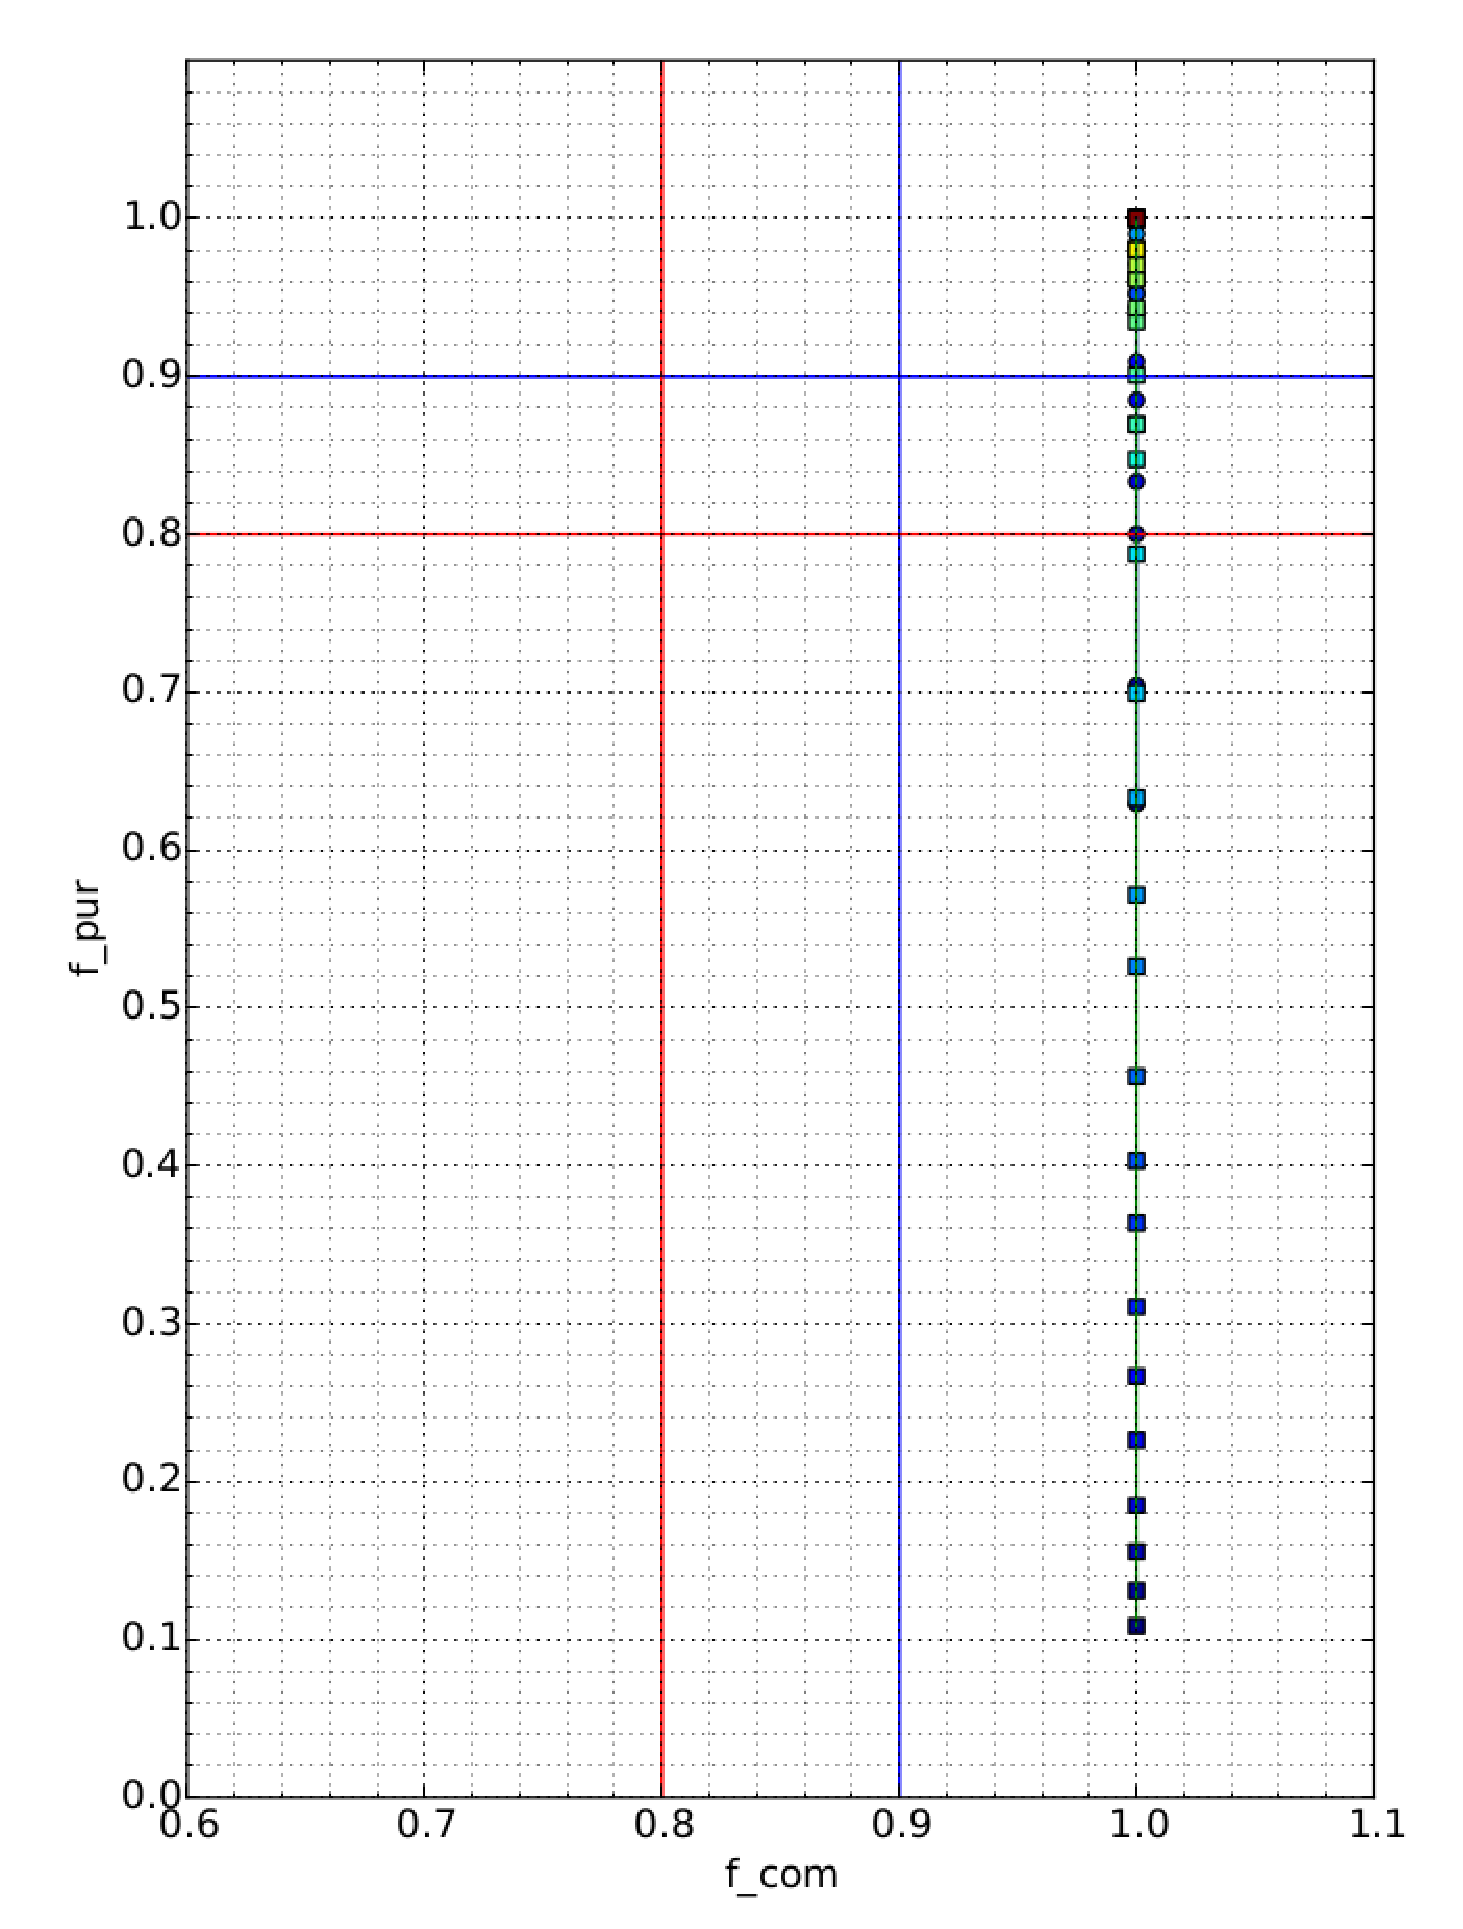
\includegraphics[width=.7\linewidth]{images/24_25_0_f.eps}
\qquad
\begin{tabular}[b]{|c|c|c|c|c|}\hline
\multicolumn{1}{|c|}{} & \multicolumn{2}{c|}{Gauss} & \multicolumn{2}{c|}{Tophat} \\
\hline \hline
Thres & Pur & Com & Pur & Com\\
\hline
1.2 & 0.63 & 1.0 & 0.1 & 1.0\\
\hline
1.4 & 0.97 & 1.0 & 0.53 & 1.0\\
\hline
1.6 & 1.0 & 1.0 & 0.94 & 1.0\\
\hline
1.8 & 1.0 & 1.0 & 1.0 & 1.0\\
\hline
2.0 & 1.0 & 1.0 & 1.0 & 1.0\\
\hline
\end{tabular}
\captionlistentry[table]{Purity against completeness values for magnitudes between 24 and 25 and a proper motion of 0.001 arcseconds per hour.}
\captionsetup{labelformat=andtable}
\caption{Purity against completeness values for magnitudes between 24 and 25 and a proper motion of 0.001 arcseconds per hour.}
\end{figure}

% Figure comment
All solutions with a purity and completeness factor higher than 0.8 are located above red lines while solutions with a factor higher than 0.9 are delimited by blue lines.

% Table comment
\par It's clear that there is a dispersion in the output by tophat filter. A better comprehension of performance behavior can be achieved taking account of true sources to total sources comparison. 

% True sources against total sources for magnitudes between 24 and 25
% and a speed of 0.001 arcseconds per hour
\subsubsection{True sources against total sources}
% Figure creation
\begin{figure}[H]
\centering
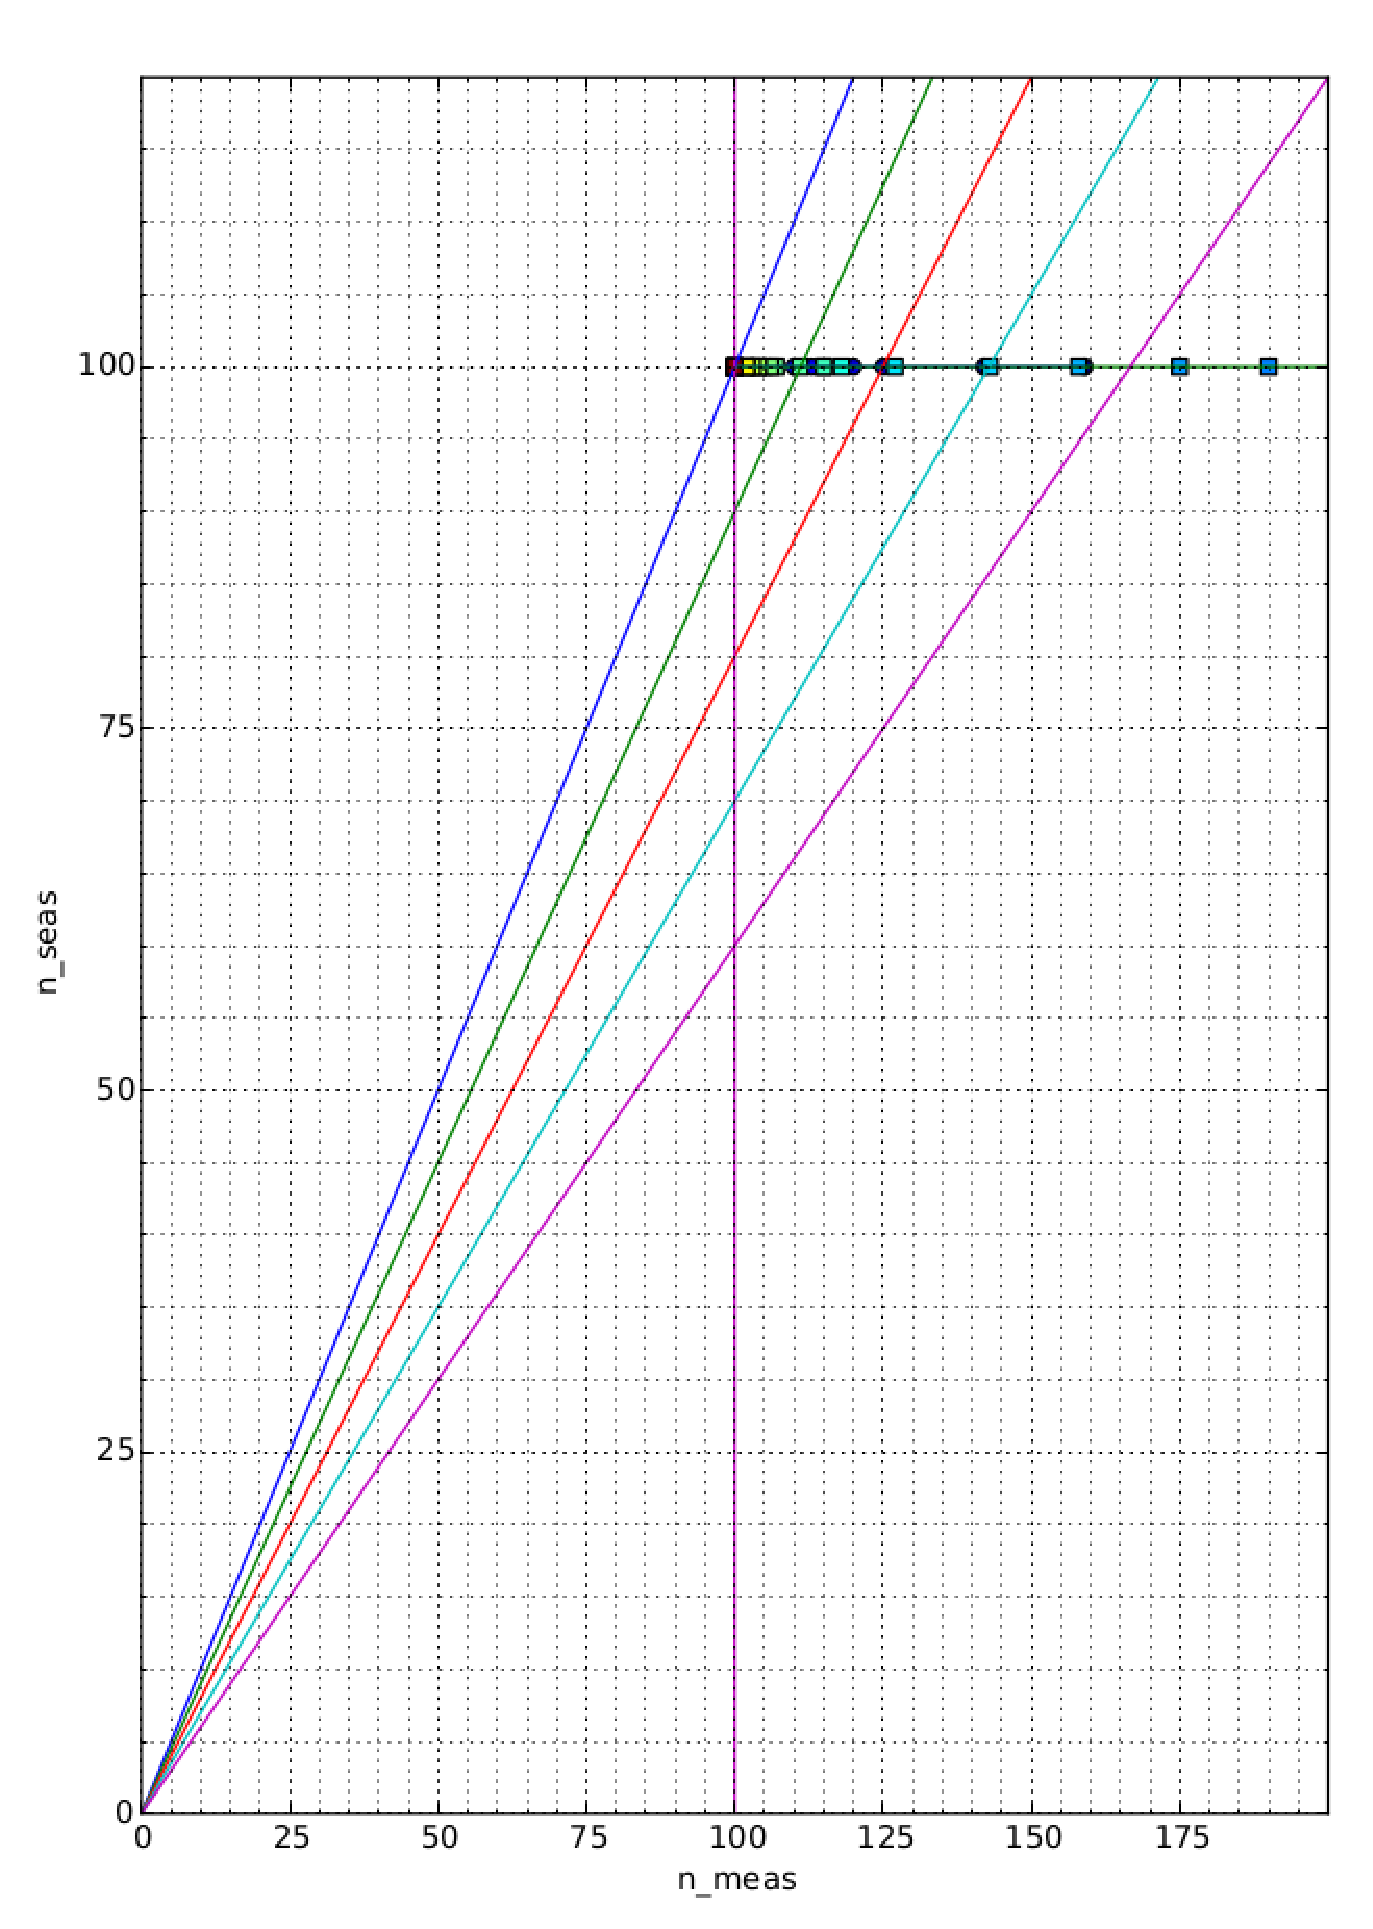
\includegraphics[width=.55\linewidth]{images/24_25_0_d.eps}
\qquad
\begin{tabular}[b]{|c|c|c|c|c|}\hline
\multicolumn{1}{|c|}{} & \multicolumn{2}{c|}{Gauss} & \multicolumn{2}{c|}{Tophat} \\
\hline \hline
Thres. & True & Total & True & Total\\
\hline
1.2 & 100 & 159 & 100 & 922\\
\hline
1.4 & 100 & 103 & 100 & 190\\
\hline
1.6 & 100 & 100 & 100 & 106\\
\hline
1.8 & 100 & 100 & 100 & 100\\
\hline
2.0 & 100 & 100 & 100 & 100\\
\hline
\end{tabular}
\captionlistentry[table]{True sources and total sources for most representative cases for magnitudes between 24 an 25 and proper motion of 0.001 arcseconds per hour.}
\captionsetup{labelformat=andtable}
\caption{True sources and total sources for most representative cases for magnitudes between 24 an 25 and proper motion of 0.001 arcseconds per hour.}
\end{figure}

% Figure comment
Because of high dispersion in the output data of topcat there are some values that are out of the plot bounds. They are not relevant for our particular study due their very low purity factor, around 0.1.
\par
Perpendicular lines show different grades of purity factor. Elements contained in blue line have a purity of 1, which is our theoretical limit. In descending order each line shows a decrement of 0.1 in purity reached.
\par
We focus our study in elements beyond red line.
% Table comment
Optimum threshold values for this particular case seems to be a number between 1.2 and 1.4 if we use the Gaussian filter and some value between 1.4 and 1.6 for tophat filter.
\par
A more concrete value will be determined looking the other scenarios.

%
% Magnitudes between 25 to 26
%
% Purity against completeness for magnitudes between 25 and 26 and
% a speed of 10 arcseconds per hour
\subsection{Magnitudes from 25 to 26}
\subsubsection{Purity against completeness}
\begin{figure}[H]
\centering
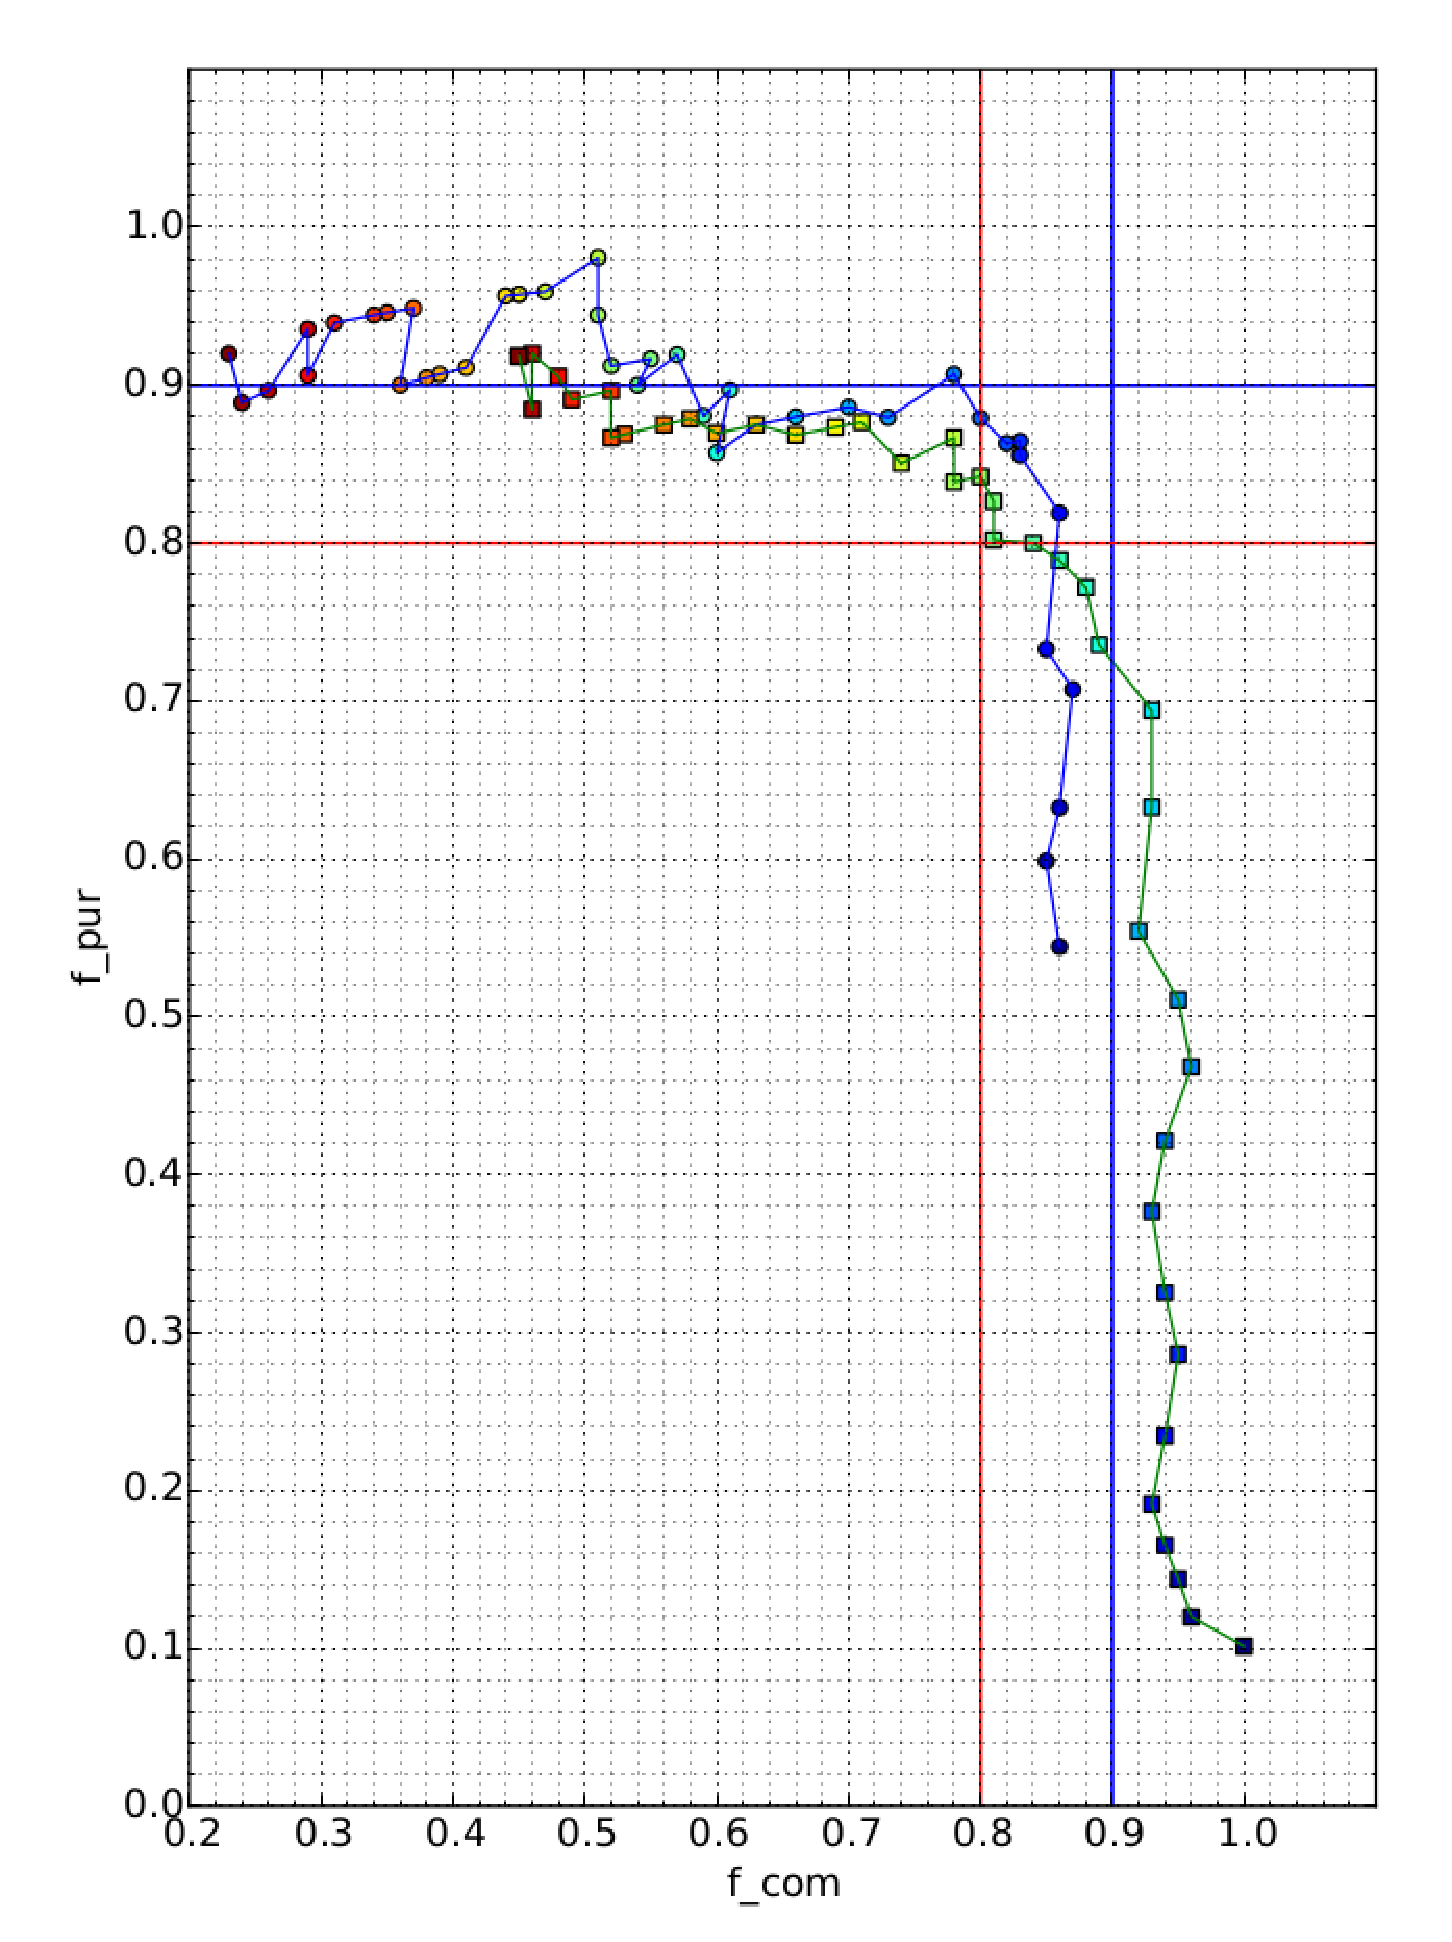
\includegraphics[width=.55\linewidth]{images/25_26_10_f.eps}
\qquad
\begin{tabular}[b]{|c|c|c|c|c|}\hline
\multicolumn{1}{|c|}{} & \multicolumn{2}{c|}{Gauss} & \multicolumn{2}{c|}{Tophat} \\
\hline \hline
Thres. & Pur. & Com. & Pur. & Com.\\
\hline
1.2 & 0.54 & 0.86 & 0.10 & 1.0\\
\hline
1.4 & 0.91 & 0.78 & 0.47 & 0.96\\
\hline
1.6 & 0.92 & 0.55 & 0.82 & 0.81\\
\hline
1.8 & 0.90 & 0.38 & 0.88 & 0.58\\
\hline
2.0 & 0.92 & 0.23 & 0.92 & 0.45\\
\hline
\end{tabular}
\captionlistentry[table]{Purity against completeness values for magnitudes between 25 and 26 and a proper motion of 10 arcseconds per hour.}
\captionsetup{labelformat=andtable}
\caption{Purity against completeness values for magnitudes between 25 and 26 and a proper motion of 10 arcseconds per hour.}
\end{figure}

% Figure comment
As we move forward to a more complicated extraction scenario we are going to lost purity if we want a relatively high purity factor.

% Table comment
Although this scenario share some particularities with the previous one, as the dispersion at tophat's output, there are some clear differences. Output curve associated to purity and completeness shows a different shape.

% True sources against total sources for magnitudes between 25 and 26
% and a speed of 10 arcseconds per hour
\subsubsection{True sources against total sources}
% Figure creation
\begin{figure}[H]
\centering
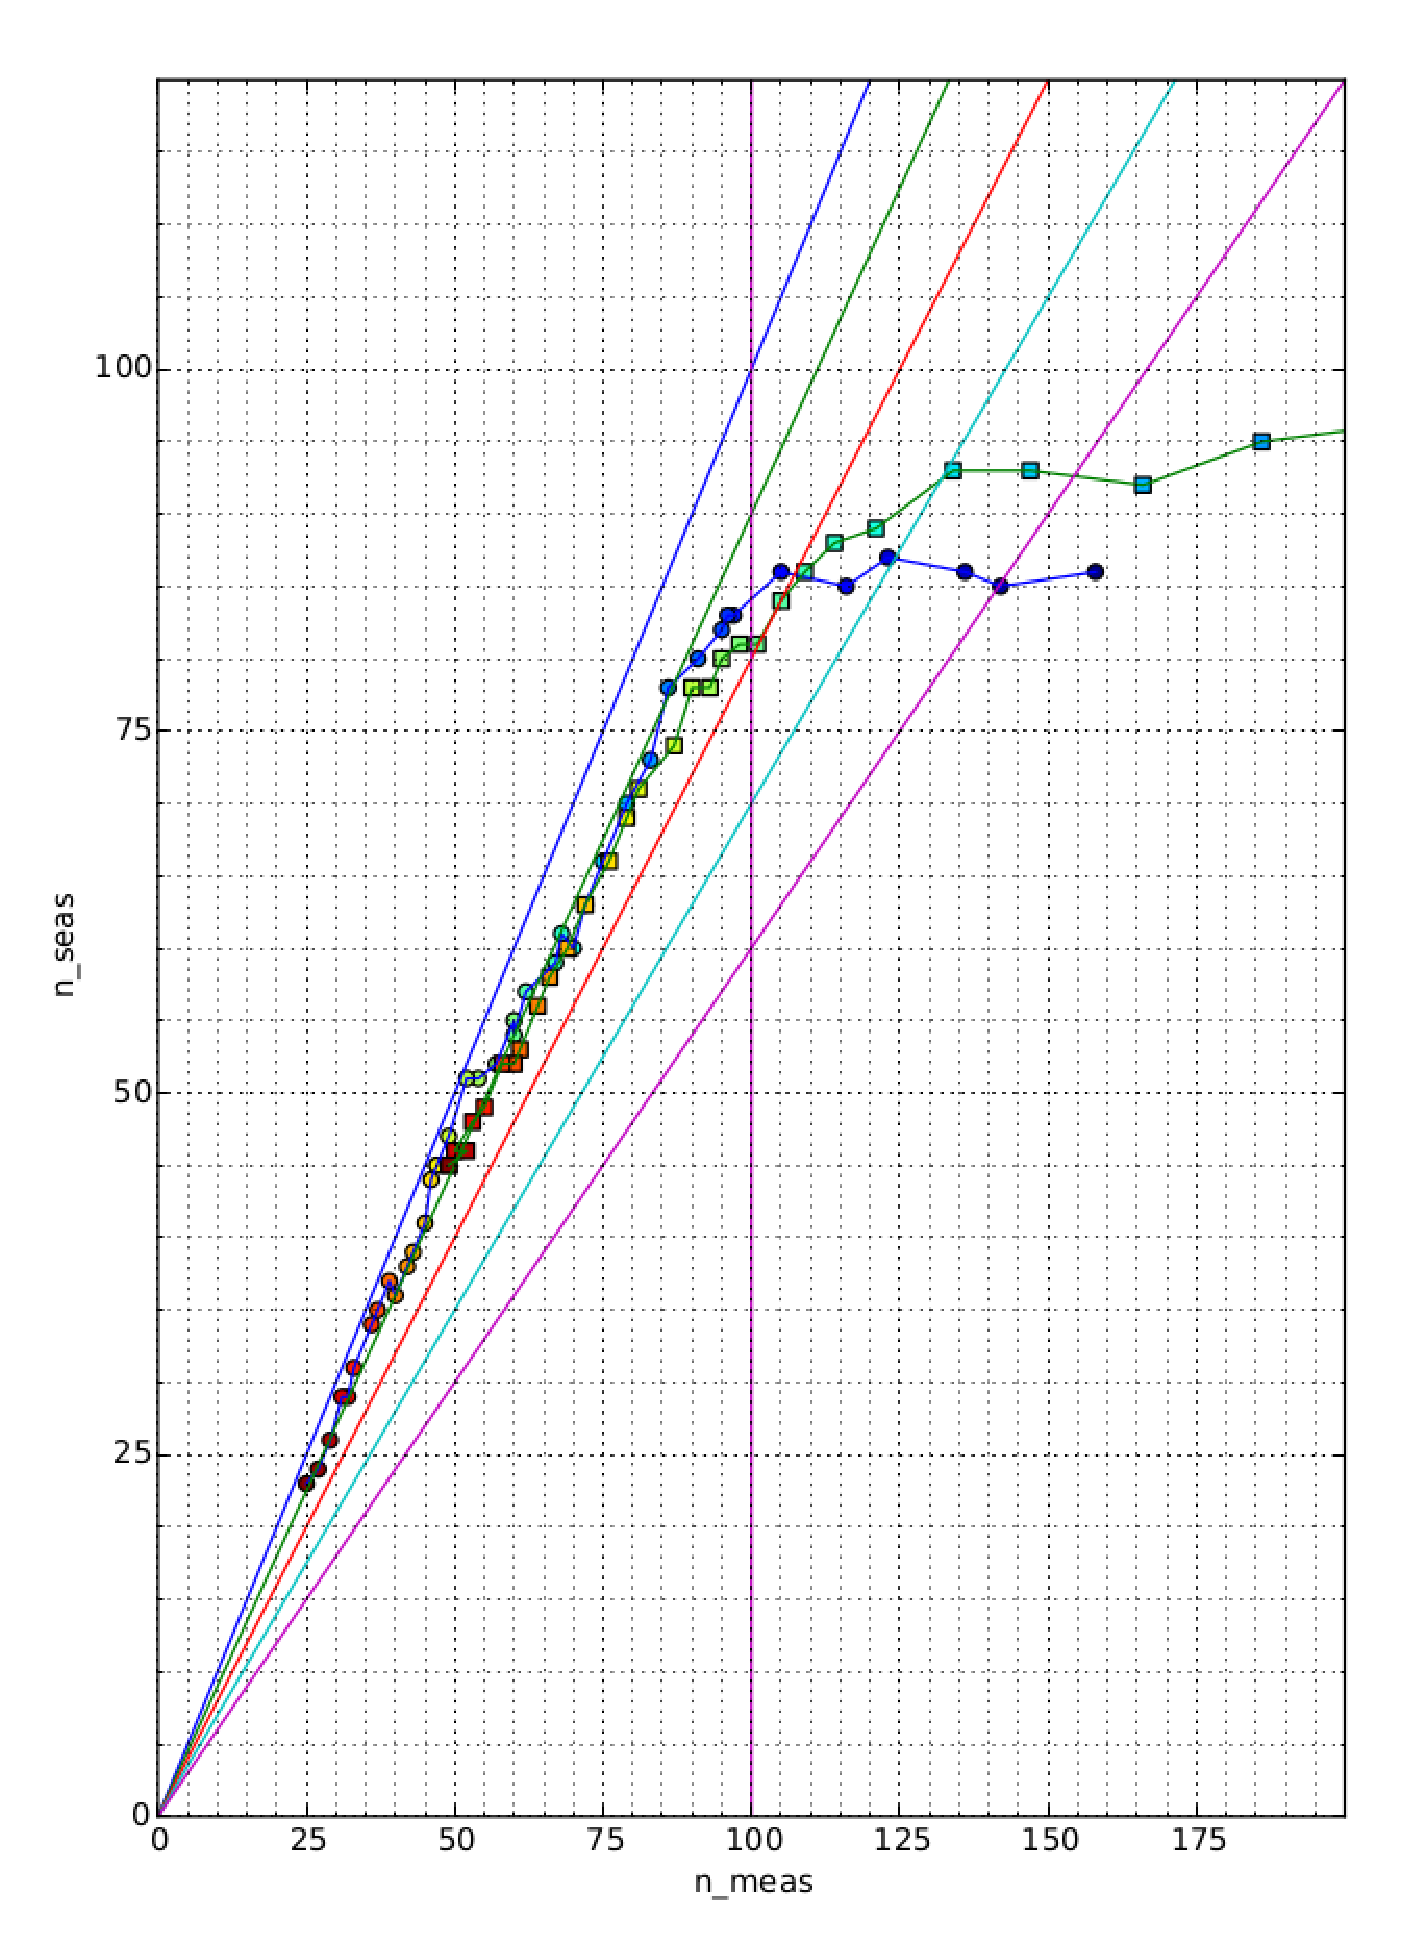
\includegraphics[width=.55\linewidth]{images/25_26_10_d.eps}
\qquad
\begin{tabular}[b]{|c|c|c|c|c|}\hline
\multicolumn{1}{|c|}{} & \multicolumn{2}{c|}{Gauss} & \multicolumn{2}{c|}{Tophat} \\
\hline \hline
Thres. & Pur. & Com. & Pur. & Com.\\
\hline
1.2 & 86 & 158 & 100 & 988\\
\hline
1.4 & 78 & 86 & 96 & 205\\
\hline
1.6 & 55 & 60 & 81 & 98\\
\hline
1.8 & 38 & 42 & 58 & 66\\
\hline
2.0 & 23 & 25 & 45 & 49\\
\hline
\end{tabular}
\captionlistentry[table]{True sources against total sources for magnitudes between 25 and 26 and a proper motion of 10 arcseconds per hour.}
\captionsetup{labelformat=andtable}
\caption{True sources against total sources for magnitudes between 25 and 26 and a proper motion of 10 arcseconds per hour.}
\end{figure}

% Figure comment
Due his high performance extracting sources some Topcat output were beyond two hundred.  

% Table comment
For a Gaussian filter scenario purity factor goes up in some point between a threshold value of 1.2 and 1.4. Beyond this point purity stays in a value close to 0.9 meanwhile completeness starts to decreases. It is make no sense to go beyond a 1.4 threshold value.
\par
Tophat filter like the Gaussian one presents a similar behavior, the main difference is that optimal threshold value move to a higher value around 1.5.

%
% Magnitudes between 26 and 27
%
\subsection{Magnitudes from 26 to 27}

% Purity against completeness for magnitudes between 26 and 27 and
% a speed of 0.001 arcseconds per hour
\subsubsection{Purity against completeness}
% Figure creation
\begin{figure}[H]
\centering
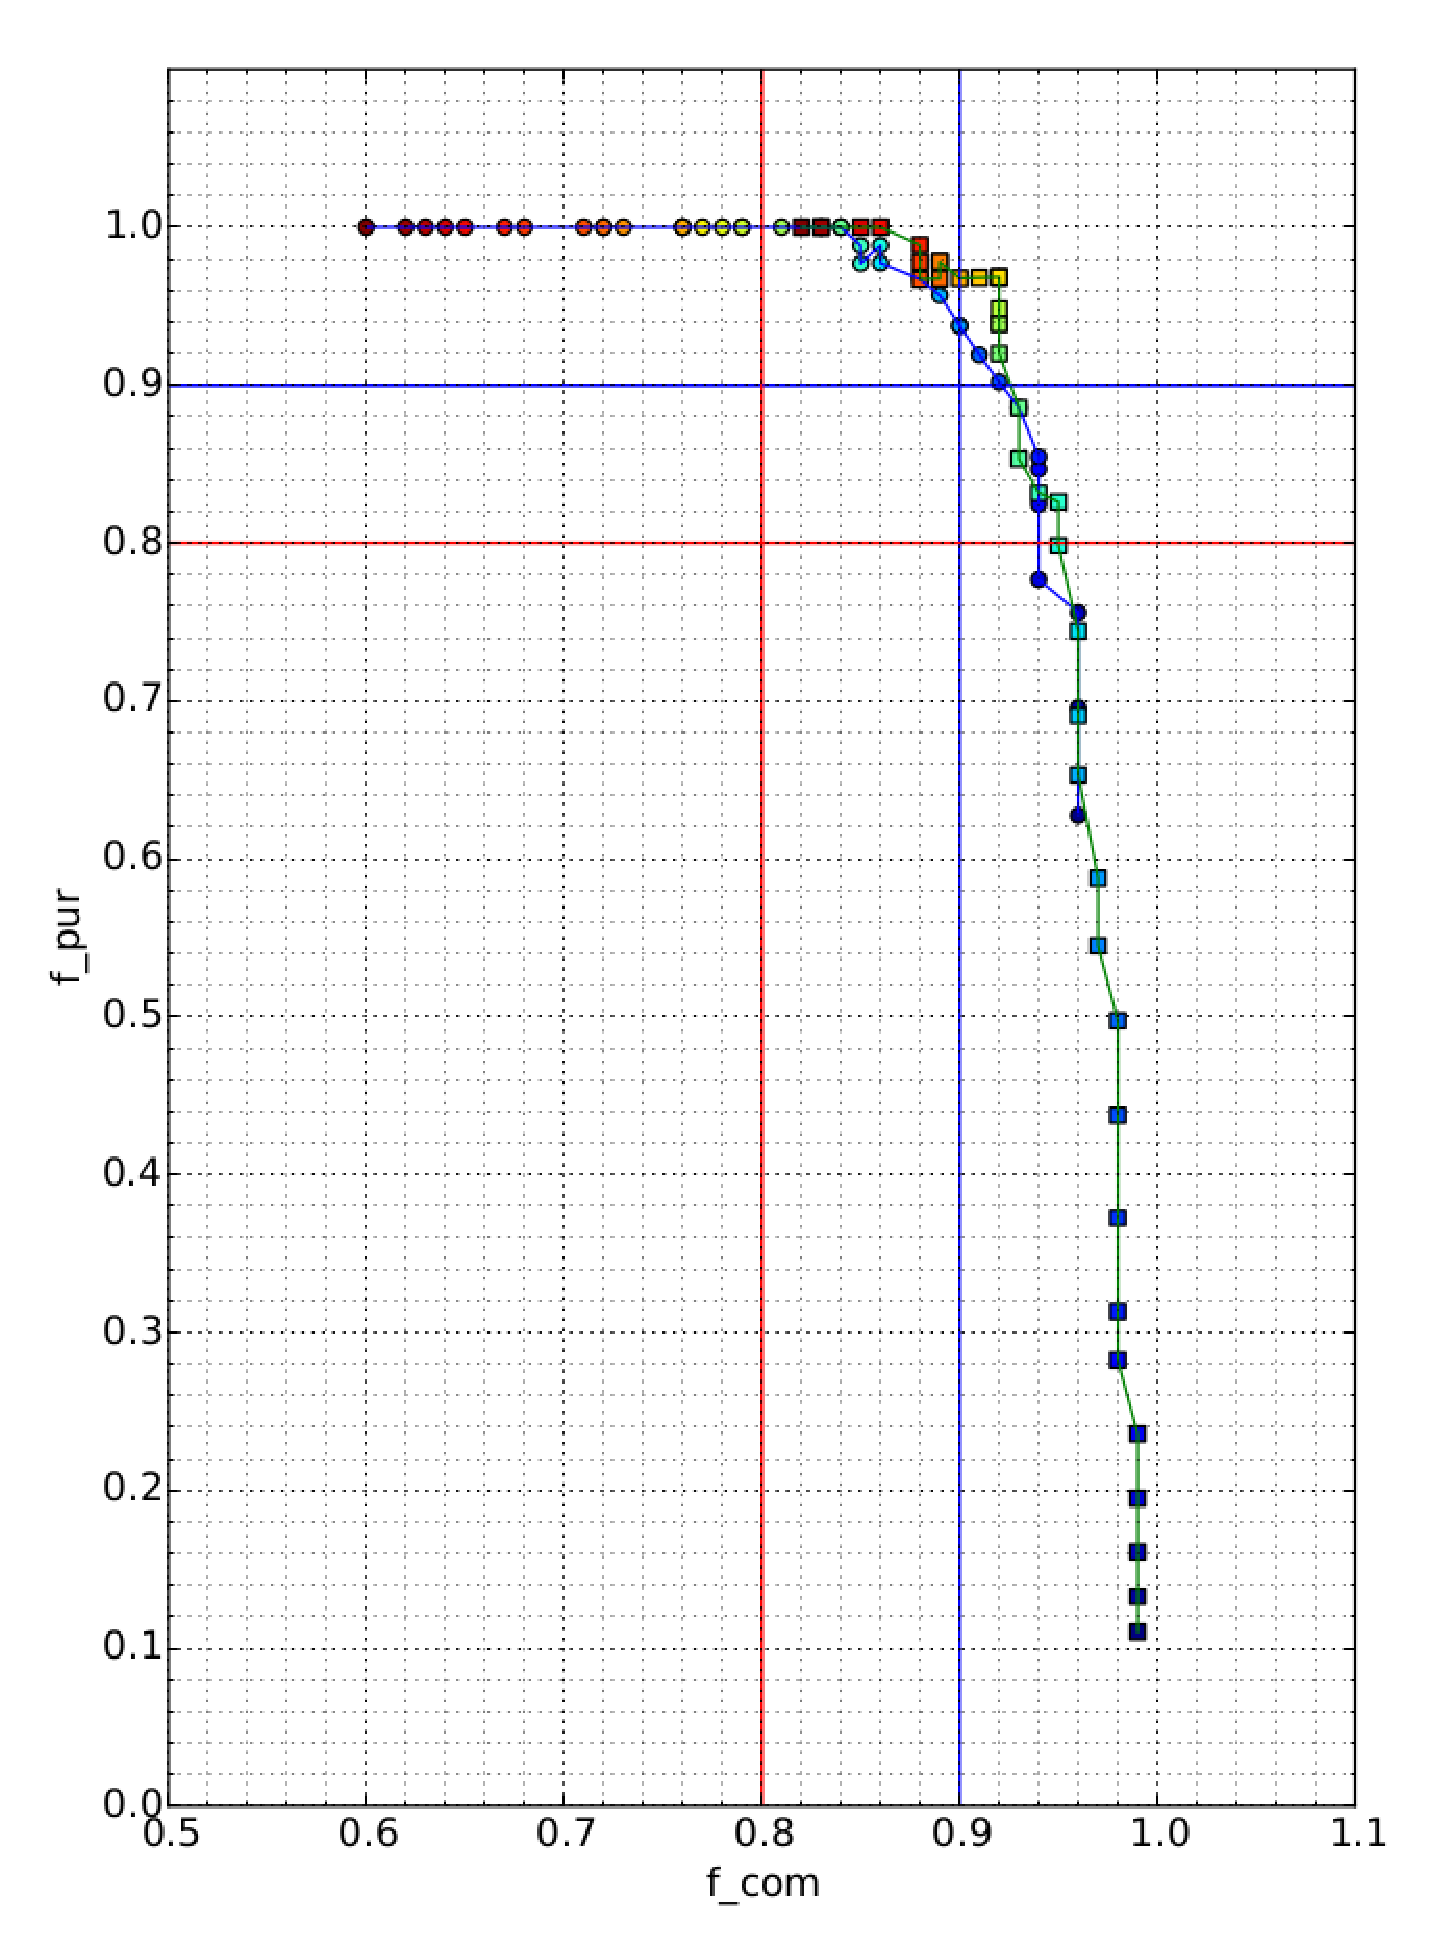
\includegraphics[width=.55\linewidth]{images/26_27_0_f.eps}
\qquad
\begin{tabular}[b]{|c|c|c|c|c|}\hline
\multicolumn{1}{|c|}{} & \multicolumn{2}{c|}{Gauss} & \multicolumn{2}{c|}{Tophat} \\
\hline \hline
Thres. & Pur. & Com. & Pur. & Com.\\
\hline
1.2 & 0.63 & 0.96 & 0.11 & 0.99\\
\hline
1.4 & 0.94 & 0.90 & 0.54 & 0.97\\
\hline
1.6 & 1.0 & 0.83 & 0.92 & 0.92\\
\hline
1.8 & 1.0 & 0.73 & 0.98 & 0.89\\
\hline
2.0 & 1.0 & 0.60 & 1.0 & 0.82\\
\hline
\end{tabular}
\captionlistentry[table]{Purity against completeness values for magnitudes between 26 and 27 and a proper motion of 0.001 arcseconds per hour.}
\captionsetup{labelformat=andtable}
\caption{Purity against completeness values for magnitudes between 26 and 27 and a proper motion of 0.001 arcseconds per hour.}
\end{figure}

% Figure comment
For this scenario output data presents a behavior very similar to previous case although curve shape looks clearer.
All results above red lines have a purity and completeness higher than 0.8. Better performance can be found above blue lines where threshold values give us factors higher than 0.9.

% True sources against total sources for magnitudes between 26 and 27
% and a speed of 0.001 arcseconds per hour
\subsubsection{True sources against total sources}
% Figure creation
\begin{figure}[H]
\centering
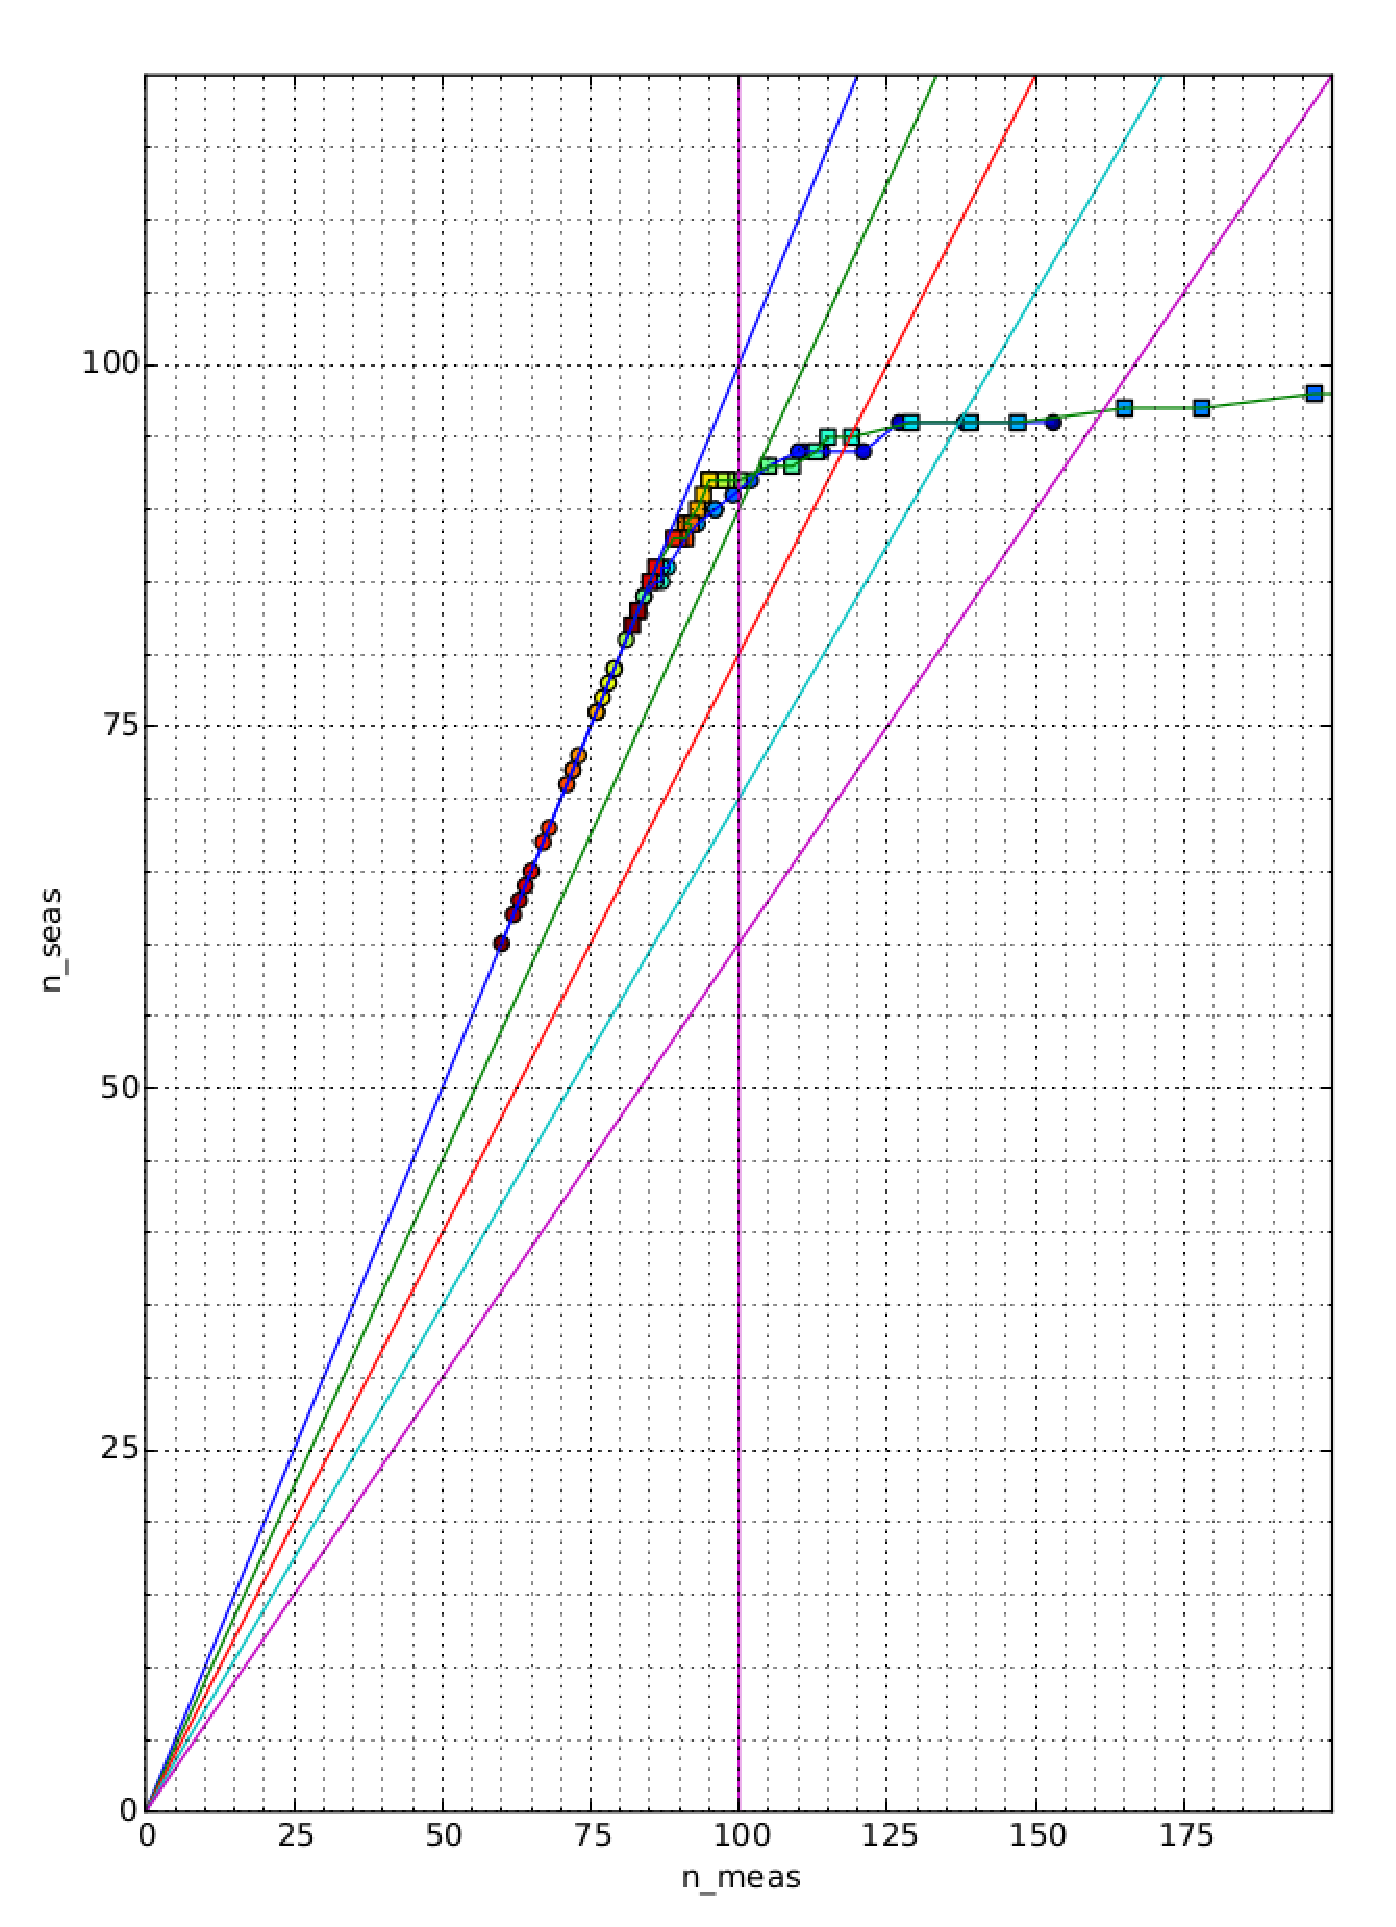
\includegraphics[width=.55\linewidth]{images/26_27_0_d.eps}
\qquad
\begin{tabular}[b]{|c|c|c|c|c|}\hline
\multicolumn{1}{|c|}{} & \multicolumn{2}{c|}{Gauss} & \multicolumn{2}{c|}{Tophat} \\
\hline \hline
Thres. & Pur. & Com. & Pur. & Com.\\
\hline
1.2 & 96 & 153 & 99 & 897\\
\hline
1.4 & 90 & 96 & 97 & 178\\
\hline
1.6 & 83 & 83 & 92 & 100\\
\hline
1.8 & 73 & 73 & 89 & 91\\
\hline
2.0 & 60 & 60 & 82 & 82\\
\hline
\end{tabular}
\captionlistentry[table]{Purity against completeness values for magnitudes between 26 and 27 and a proper motion of 0.001 arcseconds per hour.}
\captionsetup{labelformat=andtable}
\caption{Purity against completeness values for magnitudes between 26 and 27 and a proper motion of 0.001 arcseconds per hour.}
\end{figure}

% Figure comment
Extractions number using tophat filter go beyond 200 reaching values close to 900. 

% Table comment
For third we found a predictable behavior in output which give us a threshold value for gaussian filter around 1.2 and 1.4 and a threshold value between 1.4 and 1.6 for tophat filter.  

% Purity against completeness for magnitudes between 26 and 27 and
% a speed of 10 arcseconds per hour
\subsubsection{Purity against completeness}
% Figure creation
\begin{figure}[H]
\centering
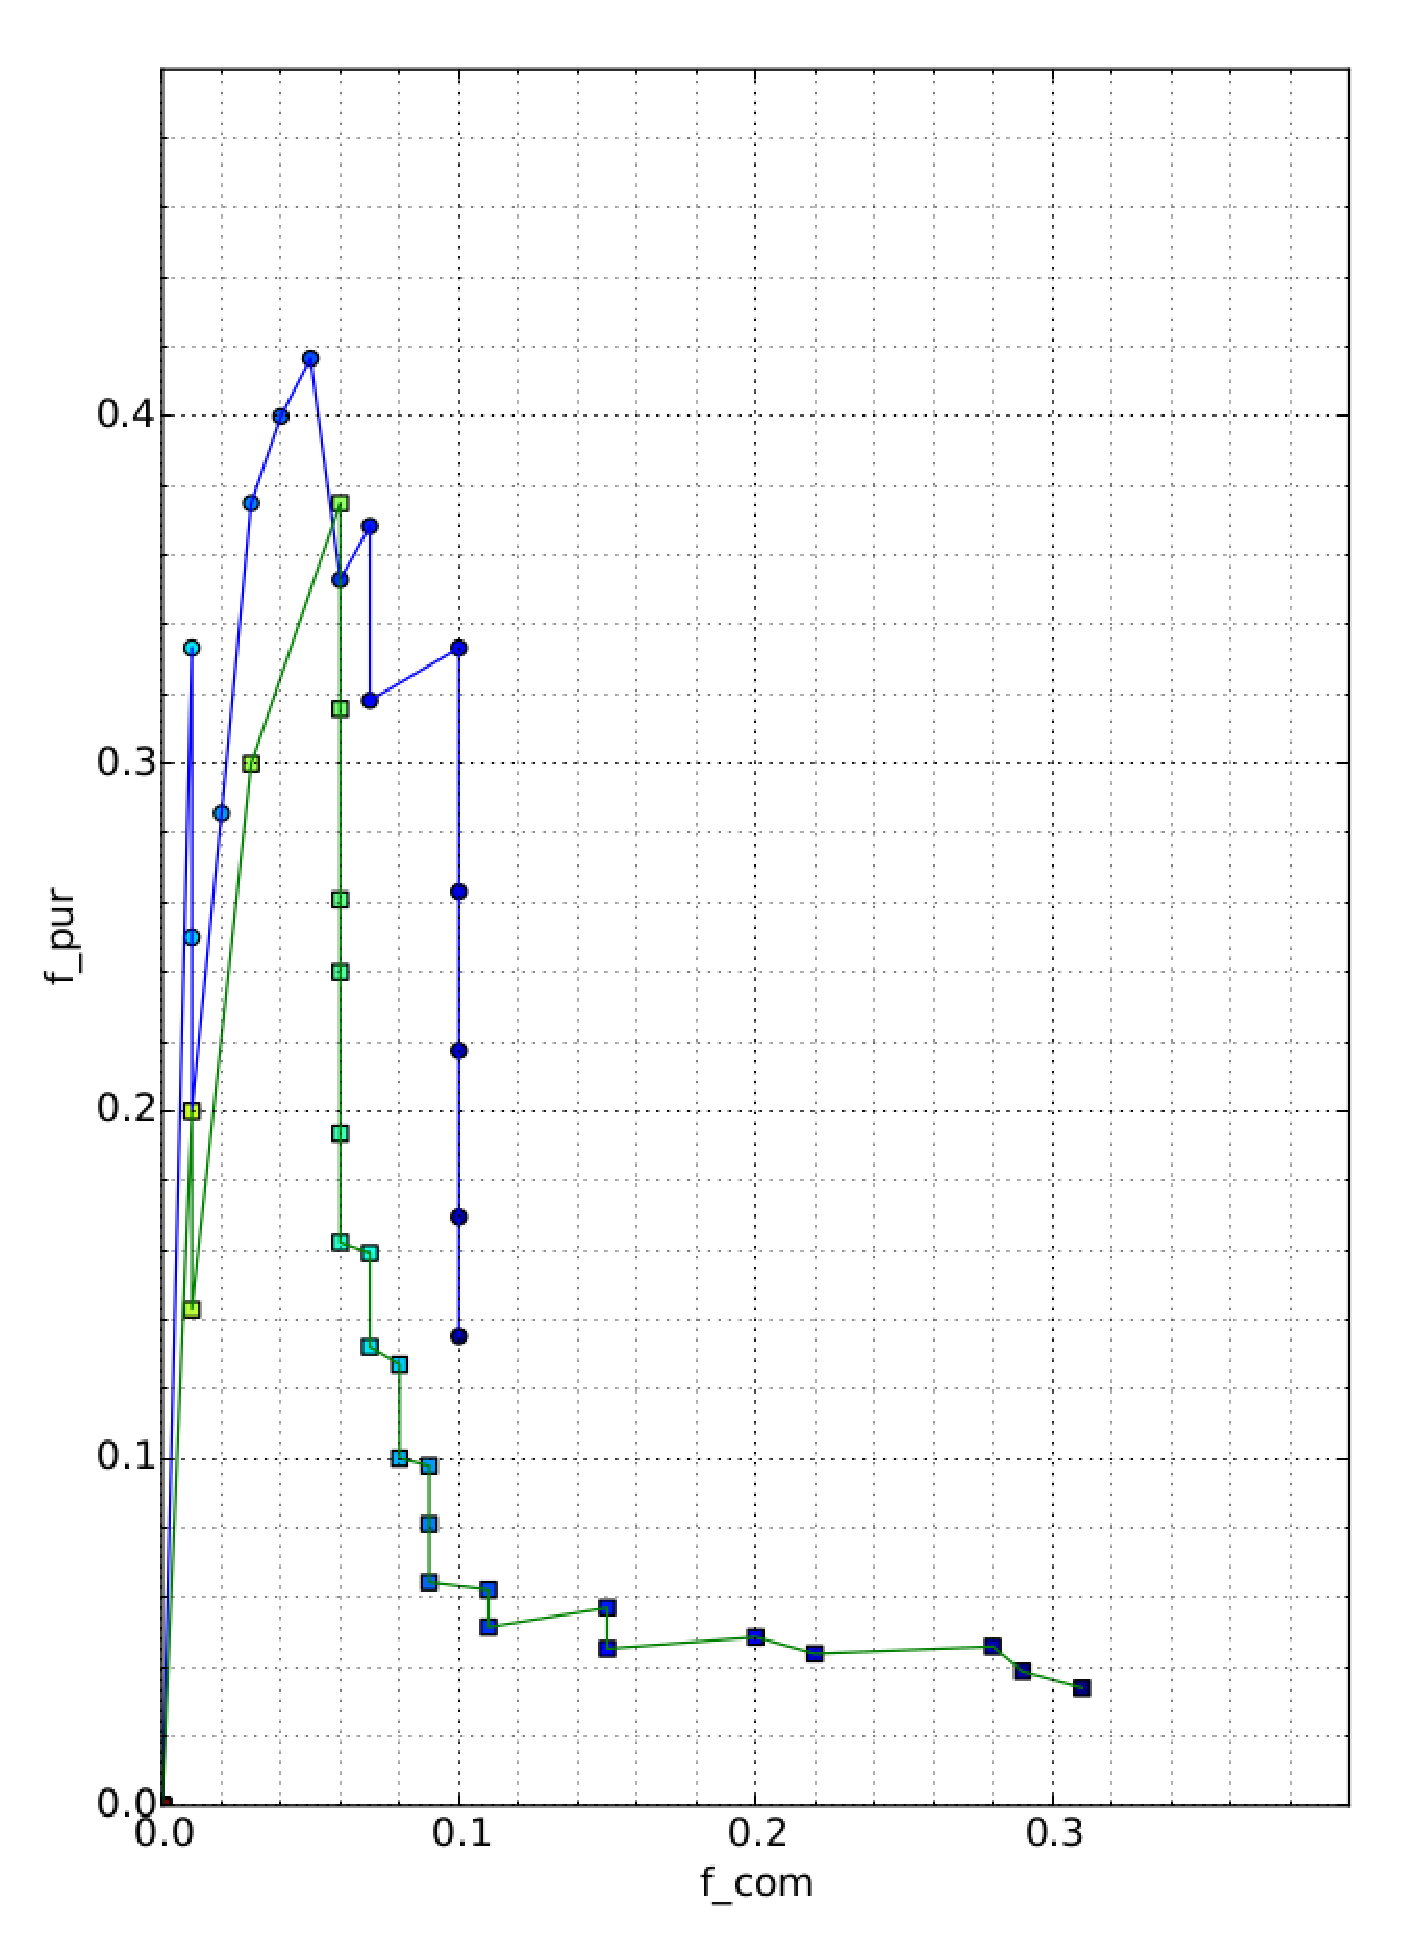
\includegraphics[width=.55\linewidth]{images/26_27_10_f.eps}
\qquad
\begin{tabular}[b]{|c|c|c|c|c|}\hline
\multicolumn{1}{|c|}{} & \multicolumn{2}{c|}{Gauss} & \multicolumn{2}{c|}{Tophat} \\
\hline \hline
Thres. & Pur. & Com. & Pur. & Com.\\
\hline
1.2 & 0.14 & 0.10 & 0.03 & 0.31\\
\hline
1.4 & 0.38 & 0.03 & 0.08 & 0.09\\
\hline
1.6 & 0 & 0 & 0.32 & 0.06\\
\hline
1.8 & 0 & 0 & 0 & 0\\
\hline
2.0 & 0 & 0 & 0 & 0\\
\hline
\end{tabular}
\captionlistentry[table]{Purity against completeness values for magnitudes between 26 and 27 and a proper motion of 10 arcseconds per hour.}
\captionsetup{labelformat=andtable}
\caption{Purity against completeness values for magnitudes between 26 and 27 and a proper motion of 10 arcseconds per hour.}
\end{figure}

% Figure comment
In this particular scenario detection for both filters become complicated. Detection of false positive over the trail of objects give us a curve with a very unpredictable shape.

% Table comment
Purity factor does not reach values higher than 0.42 and completeness shows even a littler value.

% True sources against total sources for magnitudes between 26 and 27
% and a speed of 10 arcseconds per hour
\subsubsection{True sources against total sources}

% Figure creation
\begin{figure}[H]
\centering
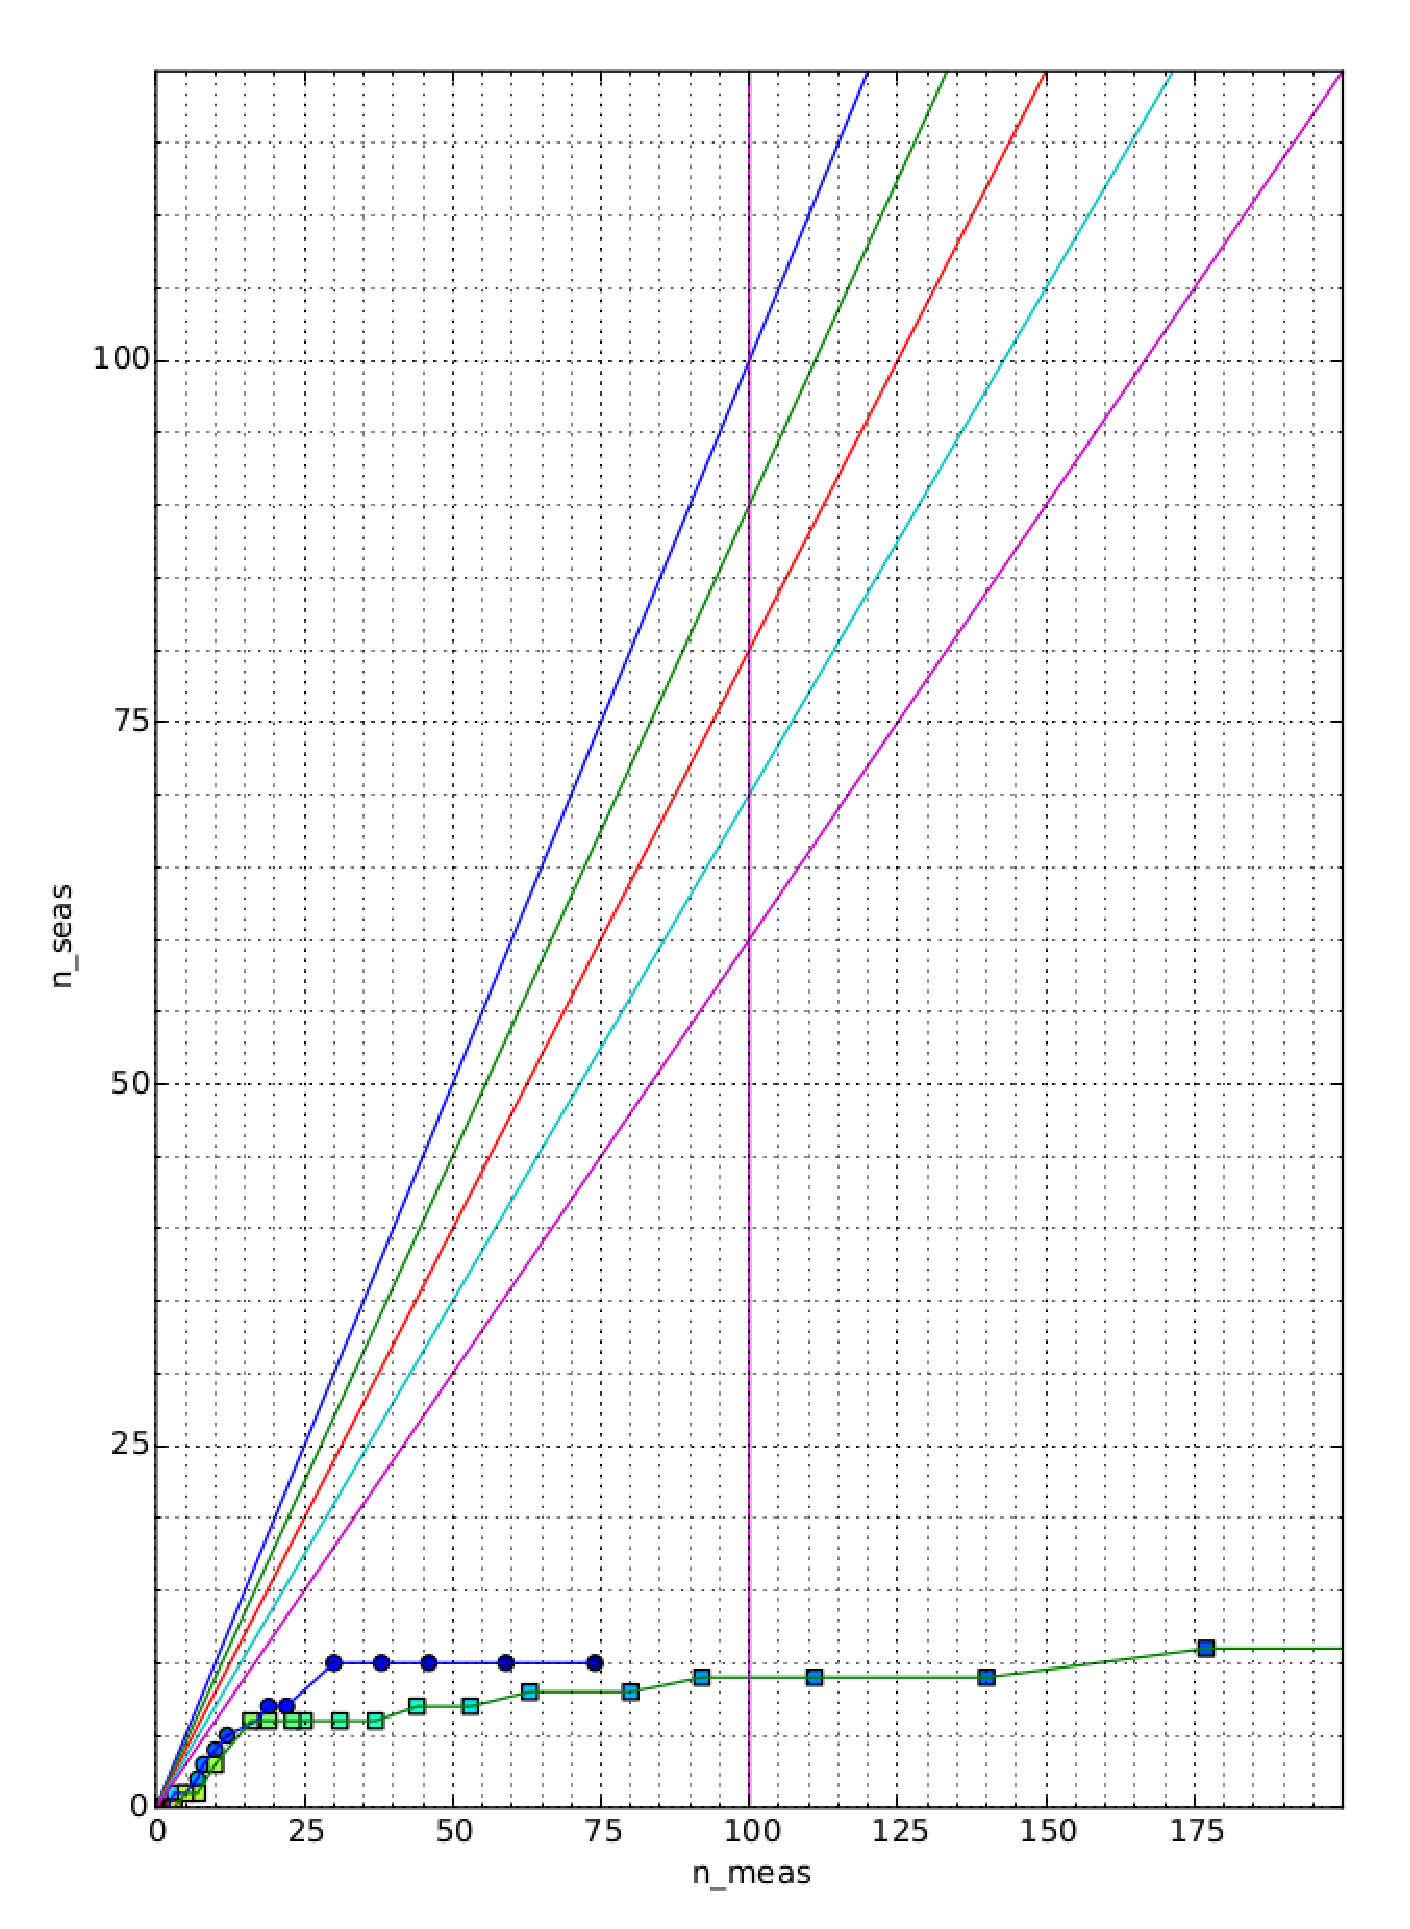
\includegraphics[width=.55\linewidth]{images/26_27_10_d.eps}
\qquad
\begin{tabular}[b]{|c|c|c|c|c|}\hline
\multicolumn{1}{|c|}{} & \multicolumn{2}{c|}{Gauss} & \multicolumn{2}{c|}{Tophat} \\
\hline \hline
Thres. & Pur. & Com. & Pur. & Com.\\
\hline
1.2 & 10 & 74 & 31 & 915\\
\hline
1.4 & 3 & 8 & 9 & 111\\
\hline
1.6 & 0 & 0 & 6 & 19\\
\hline
1.8 & 0 & 0 & 0 & 1\\
\hline
2.0 & 0 & 0 & 0 & 0\\
\hline
\end{tabular}
\captionlistentry[table]{True sources against total sources for magnitudes between 26 and 27 and a proper motion of 10 arcseconds per hour.}
\captionsetup{labelformat=andtable}
\caption{True sources against total sources for magnitudes between 26 and 27 and a proper motion of 10 arcseconds per hour.}
\end{figure}

% Figure comment
None of the outputs available 
% Table comment
Even though these last two graphs are pretty different than the previous ones factors evolution through threshold values is very similar. We set a threshold value around 1.3 for Gaussian and 1.5 for tophat filter.

\subsection{Conclusions}

\subsubsection{First scenario}
\begin{figure}[H]
\centering
\begin{tabular}{|c|c|c|c|c|}
\hline
\multicolumn{1}{|c|}{} & \multicolumn{4}{c|}{Gauss} \\
\hline \hline
Thres. & Purity & Compl. & True & Total.\\
\hline
1.2 & 0.63 & 1.0 & 100 & 159\\
\hline
1.22 & 0.70 & 1.0 & 100 & 142\\
\hline
1.24 & 0.80 & 1.0 & 100 & 125\\
\hline
1.26 & 0.83 & 1.0 & 100 & 120\\
\hline
1.28 & 0.88 & 1.0 & 100 & 113\\
\hline
1.3 & 0.91 & 1.0 & 100 & 110\\
\hline
1.32 & 0.94 & 1.0 & 100 & 106\\
\hline
1.34 & 0.95 & 1.0 & 100 & 105\\
\hline
1.36 & 0.95 & 1.0 & 100 & 105\\
\hline
1.38 & 0.96 & 1.0 & 100 & 104\\
\hline
1.4 & 0.97 & 1.0 & 100 & 103\\
\hline
\end{tabular}
\qquad
\begin{tabular}{|c|c|c|c|c|}
\hline
\multicolumn{1}{|c|}{} & \multicolumn{4}{c|}{Tophat} \\
\hline \hline
Thres. & Purity & Compl. & True & Total.\\
\hline
1.4 & 0.53 & 1.0 & 100 & 190\\
\hline
1.42 & 0.57 & 1.0 & 100 & 175\\
\hline
1.44 & 0.63 & 1.0 & 100 & 158\\
\hline
1.46 & 0.70 & 1.0 & 100 & 143\\
\hline
1.48 & 0.79 & 1.0 & 100 & 127\\
\hline
1.5 & 0.85 & 1.0 & 100 & 118\\
\hline
1.52 & 0.87 & 1.0 & 100 & 115\\
\hline
1.54 & 0.87 & 1.0 & 100 & 115\\
\hline
1.56 & 0.90 & 1.0 & 100 & 111\\
\hline
1.58 & 0.93 & 1.0 & 100 & 107\\
\hline
1.6 & 0. & 1.0 & 100 & 106\\
\hline
\end{tabular}
\captionlistentry[table]{Optimum threshold values for magnitudes between 24 and 25 and speed values of 0.001.}
\captionsetup{labelformat=andtable}
\caption{Optimum threshold values for magnitudes between 24 and 25 and speed values of 0.001.}
\end{figure}

\subsubsection{Second scenario}
\begin{figure}[H]
\centering
\begin{tabular}{|c|c|c|c|c|}
\hline
\multicolumn{1}{|c|}{} & \multicolumn{4}{c|}{Gauss} \\
\hline \hline
Thres. & Purity & Compl. & True & Total.\\
\hline
1.2 & 0.55 & 0.86 & 86 & 158\\
\hline
1.22 & 0.60 & 0.85 & 85 & 142\\
\hline
1.24 & 0.63 & 0.86 & 86 & 136\\
\hline
1.26 & 0.71 & 0.87 & 87 & 123\\
\hline
1.28 & 0.73 & 0.85 & 85 & 116\\
\hline
1.3 & 0.82 & 0.86 & 86 & 105\\
\hline
1.32 & 0.86 & 0.83 & 83 & 97\\
\hline
1.34 & 0.86 & 0.83 & 83 & 96\\
\hline
1.36 & 0.86 & 0.82 & 82 & 95\\
\hline
1.38 & 0.88 & 0.8 & 80 & 91\\
\hline
1.4 & 0.91 & 0.78 & 78 & 86\\
\hline
\end{tabular}
\qquad
\begin{tabular}{|c|c|c|c|c|}
\hline
\multicolumn{1}{|c|}{} & \multicolumn{4}{c|}{Tophat} \\
\hline \hline
Thres. & Purity & Compl. & True & Total.\\
\hline
1.4 & 0.47 & 0.96 & 96 & 205\\
\hline
1.42 & 0.51 & 0.95 & 95 & 186\\
\hline
1.44 & 0.55 & 0.92 & 92 & 166\\
\hline
1.46 & 0.63 & 0.93 & 93 & 147\\
\hline
1.48 & 0.69 & 0.93 & 93 & 134\\
\hline
1.5 & 0.74 & 0.89 & 89 & 121\\
\hline
1.52 & 0.77 & 0.88 & 88 & 114\\
\hline
1.54 & 0.79 & 0.86 & 86 & 109\\
\hline
1.56 & 0.80 & 0.84 & 84 & 105\\
\hline
1.58 & 0.80 & 0.81 & 81 & 101\\
\hline
1.6 & 0.83 & 0.81 & 81 & 98\\
\hline
\end{tabular}
\captionlistentry[table]{Optimum threshold values for magnitudes between 25 and 26 and speed values of 10}
\captionsetup{labelformat=andtable}
\caption{Optimum threshold values for magnitudes between 25 and 26 and speed values of 10}
\end{figure}

\subsubsection{Third scenario}
\begin{figure}[H]
\centering
\begin{tabular}{|c|c|c|c|c|}
\hline
\multicolumn{1}{|c|}{} & \multicolumn{4}{c|}{Gauss} \\
\hline \hline
Thres. & Purity & Compl. & True & Total.\\
\hline
1.2 & 0.63 & 0.96 & 86 & 158\\
\hline
1.22 & 0.70 & 0.96 & 85 & 142\\
\hline
1.24 & 0.76 & 0.96 & 86 & 136\\
\hline
1.26 & 0.78 & 0.94 & 87 & 123\\
\hline
1.28 & 0.82 & 0.94 & 85 & 116\\
\hline
1.3 & 0.85 & 0.94 & 86 & 105\\
\hline
1.32 & 0.85 & 0.94 & 83 & 97\\
\hline
1.34 & 0.89 & 0.93 & 83 & 96\\
\hline
1.36 & 0.90 & 0.92 & 82 & 95\\
\hline
1.38 & 0.92 & 0.91 & 80 & 91\\
\hline
1.4 & 0.94 & 0.90 & 78 & 86\\
\hline
\end{tabular}
\qquad
\begin{tabular}{|c|c|c|c|c|}
\hline
\multicolumn{1}{|c|}{} & \multicolumn{4}{c|}{Tophat} \\
\hline \hline
Thres. & Purity & Compl. & True & Total.\\
\hline
1.4 & 0.54 & 0.97 & 97 & 178\\
\hline
1.42 & 0.59 & 0.97 & 97 & 165\\
\hline
1.44 & 0.65 & 0.96 & 96 & 147\\
\hline
1.46 & 0.70 & 0.96 & 96 & 139\\
\hline
1.48 & 0.74 & 0.96 & 96 & 129\\
\hline
1.5 & 0.80 & 0.95 & 95 & 119\\
\hline
1.52 & 0.83 & 0.95 & 95 & 115\\
\hline
1.54 & 0.83 & 0.94 & 94 & 113\\
\hline
1.56 & 0.85 & 0.93 & 93 & 109\\
\hline
1.58 & 0.89 & 0.93 & 93 & 105\\
\hline
1.6 & 0.92 & 0.92 & 92 & 100\\
\hline
\end{tabular}
\captionlistentry[table]{Optimum threshold values for magnitudes between 26 and 27 and speed values of 0.001.}
\captionsetup{labelformat=andtable}
\caption{Optimum threshold values for magnitudes between 26 and 27 and speed values of 0.001.}
\end{figure}

\subsubsection{Fourth scenario}
\begin{figure}[H]
\centering
\begin{tabular}{|c|c|c|c|c|}
\hline
\multicolumn{1}{|c|}{} & \multicolumn{4}{c|}{Gauss} \\
\hline \hline
Thres. & Purity & Compl. & True & Total.\\
\hline
1.2 & 0.14 & 0.10 & 10 & 74\\
\hline
1.22 & 0.17 & 0.10 & 10 & 59\\
\hline
1.24 & 0.22 & 0.10 & 10 & 46\\
\hline
1.26 & 0.26 & 0.10 & 10 & 38\\
\hline
1.28 & 0.33 & 0.10 & 10 & 30\\
\hline
1.3 & 0.32 & 0.07 & 7 & 22\\
\hline
1.32 & 0.37 & 0.07 & 7 & 19\\
\hline
1.34 & 0.35 & 0.06 & 6 & 17\\
\hline
1.36 & 0.42 & 0.05 & 5 & 12\\
\hline
1.38 & 0.40 & 0.04 & 4 & 10\\
\hline
1.4 & 0.375 & 0.03 & 3 & 8\\
\hline
\end{tabular}
\qquad
\begin{tabular}{|c|c|c|c|c|}
\hline
\multicolumn{1}{|c|}{} & \multicolumn{4}{c|}{Tophat} \\
\hline \hline
Thres. & Purity & Compl. & True & Total.\\
\hline
1.4 & 0.08 & 0.09 & 9 & 111\\
\hline
1.42 & 0.10 & 0.09 & 9 & 92\\
\hline
1.44 & 0.10 & 0.08 & 8 & 80\\
\hline
1.46 & 0.13 & 0.08 & 8 & 63\\
\hline
1.48 & 0.13 & 0.07 & 7 & 53\\
\hline
1.5 & 0.16 & 0.07 & 7 & 44\\
\hline
1.52 & 0.16 & 0.06 & 6 & 37\\
\hline
1.54 & 0.19 & 0.06 & 6 & 31\\
\hline
1.56 & 0.24 & 0.06 & 6 & 25\\
\hline
1.58 & 0.26 & 0.06 & 6 & 23\\
\hline
1.6 & 0.32 & 0.06 & 6 & 19\\
\hline
\end{tabular}
\captionlistentry[table]{Optimum threshold values for magnitudes between 26 and 27 and speed values of 10 arcseconds per hour.}
\captionsetup{labelformat=andtable}
\caption{Optimum threshold values for magnitudes between 26 and 27 and speed values of 10 arcseconds per hour.}
\end{figure}

\subsection{Conclusion about SExtractor configuration}
A threshold value of 1.35 for analysis made using gaussian filter and 1.5 for analysis through topcat filter seems to be the best option.

\section{SCAMP analysis}
Once the best configuration for SExtractor running was chosen an analysis through the possibles SCAMP configurations will be run. A script will be run using the most important parameters of SCAMP configuration. Using the generated data a series of tables will be created in order to get an idea of the best setups available.

\subsection{Analysis approach}
Since the main objective of this study is to get an accurate astrometry from the input images the parameters involved in photometry calculations are useless in this analysis.
The relevant SCAMP configuration parameters chosen for this approach are:

\begin{itemize}
\item PIXSCALE\_MAXERR: This value is the maximum scale factor allowed in successive fields. Is shown as a percentage.
\item POSANGLE\_MAXERR: This parameter defines the range in degrees Search range (in degrees) for the position angle in the astrometric matching procedure. IMPROVE.
\item POSITION\_MAXERR: This parameter defines the range in arc-minutes of the search for the position in the astrometric matching procedure. The value is given as a float number.
\item CROSSID\_RADIUS: The maximum radius of search in arc-seconds used by the cross-identification procedures.
\end{itemize}

\subsubsection{PIXSCALE\_MAXERR}
Measured as a float number, 1.2 is the default value of this parameter. This means that the difference in the scale between different fields can be as much as twenty percent. Default value is useful for a pretty bad data. As we are dealing with an images with an excellent quality that makes no sense to use a huge margin of error. A lower values for this parameter will be tested.
\par The study values are going to be 1.05, 1.10 and 1.20.

\subsubsection{POSANGLE\_MAXERR}
Given as a float number, this value represents the degrees around the frame position angle in the WCS information allowed for each detection. 
\par More restricted values are going to try in order to reject false positive detections. For this study are going to be 0.5 and 2.5.

\subsubsection{POSITION\_MAXERR IMPROVE}
1.0 float
 1.0 is
equivalent to a range of ±1 0 around the frame position stated in the WCS information
from the original image headers.
Probaremos con valores más restrictivos con el fin de rechazar detecciones anomalas.
\par The study values are going to be 0.009, 0.045 and 0.09 (in arc-minutes) expressed in arc-seconds these values are 0.54, 2.7 and 5.4. 

\subsubsection{CROSSID\_RADIUS}
Probably the most important parameter, this value must be related to the fastest object to be detected. The default values is 2.0, this means that the maximum movement between successive fields is two arc-seconds.

% Survey times image creation
\begin{figure}[H]
\centering
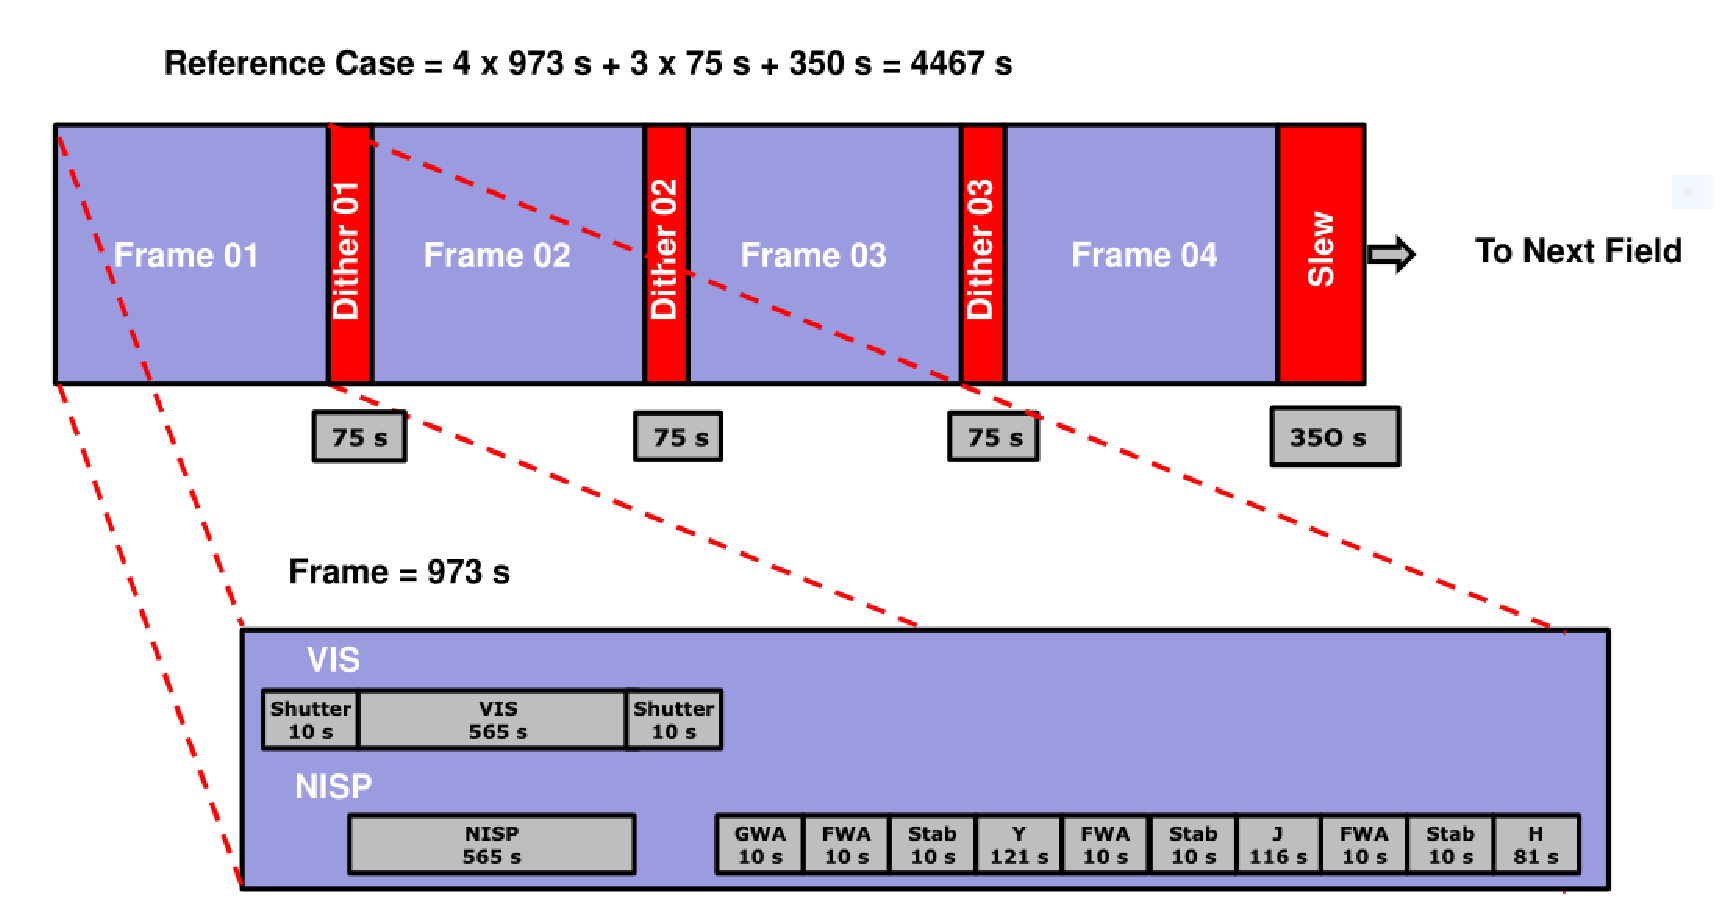
\includegraphics[width=.9\linewidth]{images/survey_times.eps}
\caption{Survey times strategy}
\end{figure}

\par For the minimum and maximum values of this parameter we must take a look of the survey time strategy. As we can notice at the graph above, taken from blablabla, time between exposures is one thousand and forty-eight seconds. As we said before sources with less than three detections will be rejected. Since we have four images per each field the maximum gap between successive detections will be 2. (?) IMPROVE
\par Distances [20 - 15 - 10]

\begin{figure}[H]
\centering
\begin{tabular}{|c|c|c|c|c|c|c|c|c|}
\hline
\multicolumn{9}{|c|}{Displacement between dithers in arc-seconds} \\
\hline \hline
dithers & 0.01 & 0.03 & 0.1 & 0.3 & 1 & 3 & 10 & 30\\
\hline \hline
1 & 0.00291 & 0.00873 & 0.0291  & 0.0873  & 0.291   & 0.873   & 2.91 & 8.73\\
\hline
2 & 0.00582 & 0.01746 & 0.0582  & 0.1746  & 0.582   & 1.746   & 5.82 & 17.46\\
\hline
\end{tabular}
\captionlistentry[table]{Maximum displacement of the same source between fields}
% \captionsetup{labelformat=andtable}
\caption{Maximum displacement of the same source between fields}
\end{figure}

\subsection{Analysis output}
Taking account of the parameters studied a list with all the possible combinations will be created. In order to make the analysis easier to understand each combination will have an unique identifier. The table with these combinations is write in the appendix A.

\subsubsection{Conclusions and final output}
Once all valuable data has been extracted the best configuration for each combination of proper motion and magnitude bin is put in a single table. For this first data review only completeness factor will be take in account. 

\begin{figure}[H]
\centering
\begin{tabular}{|c|c|c|c|c|c|c|}
\hline
\multicolumn{7}{|c|}{Best test cases}\\
\hline \hline
Proper motion & 20-21 & 21-22 & 22-23 & 23-24 & 24-25 & 25-26\\
\hline \hline
0.1 "/h & \makecell{1, 11, \\ 20, 29} & \makecell{1, 2, 3, \\ 28, 29} & \makecell{3, 30, \\ 37, 46}  & \makecell{1, 2, 3, \\ 10, 19, 38, \\ 46, 48} & \makecell{1, 10, 11, \\ 12, 20, \\ 29, 38} & \makecell{1, 2, 3, \\ 10, 11, 12, \\ 19, 20, 21, \\ 28, 29, 30, \\ 37, 38, 39, \\ 46, 47, 48}\\
\hline
0.3 "/h & \makecell{1, 2, 3 \\ 10, 11, 12 \\ 19, 20, 21 \\ 28, 29, 30 \\ 37, 38, 39 \\ 46, 47, 48} & \makecell{3, 12, 21, \\ 30, 39, 48} & \makecell{1, 2, 3 \\ 10, 11, 12 \\ 19, 20, 21 \\ 28, 29, 30 \\ 37, 38, 39 \\ 46, 47, 48} & \makecell{3, 10, 21, \\ 28, 29, 30}  & \makecell{1, 2, 3 \\ 10, 11, 12 \\ 19, 20, 21 \\ 28, 29, 30 \\ 37, 38, 39 \\ 46, 47, 48} & \makecell{1, 2, 3 \\ 10, 11, 12 \\ 19, 20, 21 \\ 28, 29, 30 \\ 37, 38, 39 \\ 46, 47, 48}\\
\hline
1 "/h & \makecell{1, 2, 3 \\ 10, 11, 12 \\ 19, 20, 21 \\ 28, 29, 30 \\ 37, 38, 39 \\ 46, 47, 48} & \makecell{1, 2, 3, \\ 10, 11, 12, \\ 28, 29, 30, \\ 37, 38, 39, \\ 46, 47, 48} & \makecell{1, 2, 3 \\ 10, 11, 12 \\ 19, 20, 21 \\ 28, 29, 30 \\ 37, 38, 39 \\ 46, 47, 48}  & \makecell{1, 2, 3 \\ 10, 11, 12 \\ 19, 20, 21 \\ 28, 29, 30 \\ 37, 38, 39 \\ 46, 47, 48}  & \makecell{1, 2, 3 \\ 10, 11, 12 \\ 19, 20, 21 \\ 28, 29, 30 \\ 37, 38, 39 \\ 46, 47, 48} & \makecell{1, 2, 3 \\ 10, 11, 12 \\ 19, 20, 21 \\ 28, 29, 30 \\ 37, 38, 39 \\ 46, 47, 48}\\
\hline
3 "/h & \makecell{1, 2, 3 \\ 10, 11, 12 \\ 19, 20, 21 \\ 28, 29, 30 \\ 37, 38, 39 \\ 46, 47, 48} & \makecell{1, 2, 3 \\ 10, 11, 12 \\ 19, 20, 21 \\ 28, 29, 30 \\ 37, 38, 39 \\ 46, 47, 48} & \makecell{1, 2, 3 \\ 10, 11, 12 \\ 19, 20, 21 \\ 28, 29, 30 \\ 37, 38, 39 \\ 46, 47, 48}  & \makecell{1, 2, 3 \\ 10, 11, 12 \\ 19, 20, 21 \\ 28, 29, 30 \\ 37, 38, 39 \\ 46, 47, 48} & \makecell{1, 2, 3 \\ 10, 11, 12 \\ 19, 20, 21 \\ 28, 29, 30 \\ 37, 38, 39 \\ 46, 47, 48} & \makecell{1, 2, 3 \\ 10, 11, 12 \\ 19, 20, 21 \\ 28, 29, 30 \\ 37, 38, 39 \\ 46, 47, 48}\\
\hline
10 "/h & \makecell{1, 2, 3 \\ 10, 11, 12 \\ 19, 20, 21 \\ 28, 29, 30 \\ 37, 38, 39 \\ 46, 47, 48} & \makecell{1, 2, 3 \\ 10, 11, 12 \\ 19, 20, 21 \\ 28, 29, 30 \\ 37, 38, 39 \\ 46, 47, 48} & \makecell{1, 2, 3 \\ 10, 11, 12 \\ 19, 20, 21 \\ 28, 29, 30 \\ 37, 38, 39 \\ 46, 47, 48} & \makecell{1, 2, 3 \\ 10, 11, 12 \\ 19, 20, 21 \\ 28, 29, 30 \\ 37, 38, 39 \\ 46, 47, 48} & \makecell{1, 2, 3 \\ 10, 11, 12 \\ 19, 20, 21 \\ 28, 29, 30 \\ 37, 38, 39 \\ 46, 47, 48} & \makecell{1, 2, 3 \\ 10, 11, 12 \\ 19, 20, 21 \\ 28, 29, 30 \\ 37, 38, 39 \\ 46, 47, 48}\\
\hline
\end{tabular}
\captionlistentry[table]{Best test cases for purity and completeness factors}
\caption{Best test cases for purity and completeness factors}
\end{figure}

En la tabla superior están 

\begin{figure}[H]
\centering
\begin{tabular}{|c|c|c|c|c|c|c|c|}
\hline
\multicolumn{8}{|c|}{Best test cases}\\
\hline \hline
Proper motion & Test & 20-21 & 21-22 & 22-23 & 23-24 & 24-25 & 25-26\\
\hline \hline
0.1 "/h & 1 & 0.09 & 0.04 & 0.02  & 0.01 & 0.01 & 0.03\\
\cline{2-8}
& 3 & 0.09 & 0.04 & 0.02  & 0.01 & 0.01 & 0.03\\
\cline{2-8}
& 29 & 0.09 & 0.04 & 0.02  & 0.01 & 0.01 & 0.03\\
\hline
0.3 "/h & 1 & \textbf{0.17} & 0.09 & 0.05 & 0.02 & 0.01 & 0.01\\
\cline{2-8}
& 3 & 0.16 & 0.09 & \textbf{0.09}  & 0.02 & 0.01 & 0.01\\
\cline{2-8}
& 29 & \textbf{0.17} & 0.09 & 0.05 & 0.02 & 0.01 & \textbf{0.03}\\
\hline
1.0 "/h & 1 & \textbf{0.59} & 0.38 & \textbf{0.21} & 0.17 & \textbf{0.12} & 0.09\\
\cline{2-8}
& 3 & 0.56 & \textbf{0.39} & \textbf{0.21}  & 0.17 & \textbf{0.12} & 0.09\\
\cline{2-8}
& 29 & \textbf{0.59} & 0.38 & 0.2 & \textbf{0.18} & 0.11 & 0.09\\
\hline
3.0 "/h & 1 & \textbf{0.65} & 0.8 & 0.9 & \textbf{0.91} & \textbf{0.7} & 0.86\\
\cline{2-8}
& 3 & 0.63 & 0.8 & 0.9  & 0.8 & \textbf{0.7} & 0.86\\
\cline{2-8}
& 29 & \textbf{0.65} & 0.8 & \textbf{0.95} & 0.87 & 0.67 & \textbf{0.9}\\
\hline
10.0 "/h & 1 & 1.0 & 0.93 & 1.0 & 1.0 & 1.0 & 1.0\\
\cline{2-8}
& 3 & 1.0 & 0.93 & 1.0  & 1.0 & 1.0 & 1.0\\
\cline{2-8}
& 29 & 1.0 & 0.93 & 1.0  & 1.0 & 1.0 & 1.0\\
\hline
\end{tabular}
\captionlistentry[table]{Best test cases for purity and completeness factors}
\caption{Best test cases for purity and completeness factors}
\end{figure}

In the above table best purity factors are written in bold type.

1604 s - 1
1500 s - 29

\begin{figure}[H]
\centering
\begin{tabular}{|c|c|c|c|c|c|c|c|c|c|c|c|c|}
\hline
\multicolumn{1}{|c|}{} & \multicolumn{2}{|c|}{20-21} & \multicolumn{2}{|c|}{21-22} & \multicolumn{2}{|c|}{22-23} & \multicolumn{2}{|c|}{23-24} & \multicolumn{2}{|c|}{24-25} & \multicolumn{2}{|c|}{25-26}\\
\hline \hline
 & f\_pur & f\_com & f\_pur & f\_com & f\_pur & f\_com & f\_pur & f\_com & f\_pur & f\_com & f\_pur & f\_com \\
\hline
0.1 & 0.09 & 0.92 & 0.04 & 0.88 & 0.02 & 0.84 & 0.01 & 0.88 & 0.01 & 0.91 & 0.03 & 0.93\\
\hline
0.3 & 0.17 & 0.96 & 0.09 & 0.87 & 0.05 & 0.92 & 0.02 & 0.88 & 0.01 & 0.74 & 0.01 & 0.78\\
\hline
1.0 & 0.59 & 0.95 & 0.38 & 0.95 & 0.2 & 0.85 & 0.18 & 0.92 & 0.11 & 0.95 & 0.09 & 0.88\\
\hline
3.0 & 0.65 & 1.0 & 0.8 & 0.89 & 0.95 & 0.95 & 0.87 & 0.91 & 0.67 & 0.88 & 0.9 & 0.86\\
\hline
10.0 & 1.0 & 0.91 & 0.93 & 0.87 & 1.0 & 0.93 & 1.0 & 0.75 & 1.0 & 1.0 & 1.0 & 1.0\\
\hline
\end{tabular}
\captionlistentry[table]{pixscale\_maxerr: 1.10 posangle\_maxerr: 2.5 position\_maxerr: 0.045 crossid\_radius: 10}
\caption{pixscale\_maxerr: 1.10 posangle\_maxerr: 2.5 position\_maxerr: 0.045 crossid\_radius: 10}
\end{figure}

\par The only relevant factor was...

\par The values of purity, completeness and detection rate factors obtained using the final configuration are show in the following table. As we can see these values are far away of an ideal situation. A later filter process seems to be necessary. 

\section{Filtering}
Data from SExtractor and SCAMP catalogues are going to be used in the filter process. In each section of this chapter a different data correlation is going to be tested. These data correlations are going to be used to rejects false positives. The advantages and disadvantages of every filter will be discussed in order to get the best pipeline performance. 

\subsection{Movement coherence filter}
Taken from a previous study\footnote{Max} this filter is the first attempt to improve factor values. This filter tries to fit the displacement in one axis versus the increased time. In the same amount of time the object must have the same displacement.

\subsubsection{Data and adjustment process}
A weighted least squares regression will be performed. This regression allow us to introduce the position determination error. The method chosen to accept or decline a source will be a chi-squared test. This is used to determine whether there is a difference between the expected movement and the observed displacement. Two different cases are going to be studied.
\begin{itemize}
\item right ascension and declination adjusted: in this case a regression between right ascension and epoch and another between declination and epoch will be created. Both adjustments must have a chi-squared value higher than our reference variable.
\item right ascension or declination adjusted: in this way only one regression must have a right chi-squared value. 
\end{itemize}
\par The chi-squared reference variable is going to be obtained in this analysis. A set of values is going to be tested. The best number should be the one that rejects enough false positives without letting out true sources. In this study 0.85, 0.9 and 0.95 are going to be tested.

\subsubsection{Both axis adjusted}
Instead of showing the new purity and completeness values the difference between old and new ones will be shown. This approach can show in a easier way the performance of this filter process.

\begin{figure}[H]
\centering
\begin{tabular}{|c|c|c|c|c|c|c|c|c|c|c|c|c|}
\hline
\multicolumn{1}{|c|}{} & \multicolumn{2}{|c|}{20-21} & \multicolumn{2}{|c|}{21-22} & \multicolumn{2}{|c|}{22-23} & \multicolumn{2}{|c|}{23-24} & \multicolumn{2}{|c|}{24-25} & \multicolumn{2}{|c|}{25-26}\\
\hline \hline
"/h & f\_pur & f\_com & f\_pur & f\_com & f\_pur & f\_com & f\_pur & f\_com & f\_pur & f\_com & f\_pur & f\_com \\
\hline
0.1 & 0.17 & -0.71 & 0.05 & -0.72 & 0.04 & -0.63 & 0.0 & -0.82 & 0.03 & -0.77 & 0.01 & -0.79\\
\hline
0.3 & 0.26 & -0.53 & 0.24 & -0.34 & 0.13 & -0.57 & 0.05 & -0.5 & 0.05 & -0.3 & 0.05 & -0.31\\
\hline
1.0 & 0.3 & -0.15 & 0.47 & -0.14 & 0.47 & -0.15 & 0.3 & 0.3 & 0.26 & -0.3 & 0.28 & -0.2\\
\hline
3.0 & 0.11 & -0.06 & 0.08 & -0.11 & 0.0 & 0.0 & 0.08 & -0.09 & 0.33 & -0.19 & 0.1 & -0.17\\
\hline
10.0 & 0.0 & 0.0 & 0.0 & 0.0 & 0.0 & -0.07 & 0.0 & 0.0 & 0.0 & 0.0 & 0.0 & 0.0\\
\hline
\end{tabular}
\captionlistentry[table]{Purity and completeness factor for a chi-squared value of 0.85 with both axis adjusted}
\caption{Purity and completeness factor for a chi-squared value of 0.85 with both axis adjusted}
\end{figure}

\begin{figure}[H]
\centering
\begin{tabular}{|c|c|c|c|c|c|c|c|c|c|c|c|c|}
\hline
\multicolumn{1}{|c|}{} & \multicolumn{2}{|c|}{20-21} & \multicolumn{2}{|c|}{21-22} & \multicolumn{2}{|c|}{22-23} & \multicolumn{2}{|c|}{23-24} & \multicolumn{2}{|c|}{24-25} & \multicolumn{2}{|c|}{25-26}\\
\hline \hline
"/h & f\_pur & f\_com & f\_pur & f\_com & f\_pur & f\_com & f\_pur & f\_com & f\_pur & f\_com & f\_pur & f\_com \\
\hline
0.1 & 0.02 & -0.88 & 0.1 & -0.72 & 0.04 & -0.68 & 0.01 & -0.82 & 0.03 & -0.82 & 0.05 & -0.89\\
\hline
0.3 & 0.33 & -0.57 & 0.25 & -0.47 & 0.21 & -0.6 & 0.07 & -0.57 & 0.07 & -0.37 & 0.05 & -0.65\\
\hline
1.0 & 0.29 & -0.2 & 0.46 & -0.19 & 0.52 & -0.2 & 0.4 & -0.34 & 0.35 & -0.3 & 0.29 & -0.38\\
\hline
3.0 & 0.11 & -0.06 & 0.08 & -0.11 & 0.0 & 0.0 & 0.08 & -0.09 & 0.33 & -0.19 & 0.05 & 0.0\\
\hline
10.0 & 0.0 & 0.0 & 0.0 & 0.0 & 0.0 & -0.07 & 0.0 & 0.0 & 0.0 & 0.0 & 0.0 & -0.5\\
\hline
\end{tabular}
\captionlistentry[table]{Purity and completeness factor for a chi-squared value of 0.9 with both axis adjusted}
\caption{Purity and completeness factor for a chi-squared value of 0.9 with both axis adjusted}
\end{figure}

\begin{figure}[H]
\centering
\begin{tabular}{|c|c|c|c|c|c|c|c|c|c|c|c|c|}
\hline
\multicolumn{1}{|c|}{} & \multicolumn{2}{|c|}{20-21} & \multicolumn{2}{|c|}{21-22} & \multicolumn{2}{|c|}{22-23} & \multicolumn{2}{|c|}{23-24} & \multicolumn{2}{|c|}{24-25} & \multicolumn{2}{|c|}{25-26}\\
\hline \hline
"/h & f\_pur & f\_com & f\_pur & f\_com & f\_pur & f\_com & f\_pur & f\_com & f\_pur & f\_com & f\_pur & f\_com \\
\hline
0.1 & 0.02 & -0.88 & 0.16 & -0.76 & 0.07 & -0.73 & -0.01 & -0.88 & 0.03 & -0.86 & 0.09 & -0.89\\
\hline
0.3 & 0.39 & -0.74 & 0.32 & -0.64 & 0.32 & -0.65 & 0.02 & -0.8 & 0.11 & -0.48 & 0.04 & -0.74\\
\hline
1.0 & 0.26 & -0.4 & 0.5 & -0.24 & 0.66 & -0.25 & 0.47 & -0.46 & 0.6 & -0.35 & 0.41 & -0.44\\
\hline
3.0 & 0.19 & -0.06 & 0.07 & -0.17 & 0.0 & -0.05 & 0.08 & -0.09 & 0.33 & -0.26 & 0.1 & -0.05\\
\hline
10.0 & 0.0 & 0.0 & -0.01 & -0.07 & 0.0 & -0.07 & 0.0 & 0.0 & 0.0 & 0.0 & 0.0 & -0.5\\
\hline
\end{tabular}
\captionlistentry[table]{Purity and completeness factor for a chi-squared value of 0.95 with both axis adjusted}
\caption{Purity and completeness factor for a chi-squared value of 0.95 with both axis adjusted}
\end{figure}

As can be see the last case presents the biggest losses in completeness factor values while the first one, figure nineteen, looks like the best option for this approach.

\subsubsection{One single axis adjusted}
Now, the next study case will be tested. In this way only one chi squared value must be achieved in order to accept a source.

\begin{figure}[H]
\centering
\begin{tabular}{|c|c|c|c|c|c|c|c|c|c|c|c|c|}
\hline
\multicolumn{1}{|c|}{} & \multicolumn{2}{|c|}{20-21} & \multicolumn{2}{|c|}{21-22} & \multicolumn{2}{|c|}{22-23} & \multicolumn{2}{|c|}{23-24} & \multicolumn{2}{|c|}{24-25} & \multicolumn{2}{|c|}{25-26}\\
\hline \hline
"/h & f\_pur & f\_com & f\_pur & f\_com & f\_pur & f\_com & f\_pur & f\_com & f\_pur & f\_com & f\_pur & f\_com \\
\hline
0.1 & 0.03 & -0.34 & 0.02 & -0.32 & 0.00 & -0.31 & 0.01 & -0.12 & 0.01 & -0.36 & 0.03 & -0.45\\
\hline
0.3 & 0.06 & -0.18 & 0.07 & -0.04 & 0.04 & -0.06 & 0.01 & -0.11 & 0.01 & -0.06 & 0.01 & -0.21\\
\hline
1.0 & 0.17 & 0.0 & 0.19 & 0.0 & 0.17 & 0.0 & 0.1 & 0.0 & 0.12 & 0.0 & 0.06 & -0.07\\
\hline
3.0 & 0.09 & 0.0 & 0.09 & 0.0 & 0.0 & 0.0 & 0.08 & 0.0 & 0.26 & 0.0 & 0.05 & 0.0\\
\hline
10.0 & 0.0 & 0.0 & 0.0 & 0.0 & 0.0 & 0.0 & 0.0 & 0.0 & 0.0 & 0.0 & 0.0 & 0.0\\
\hline
\end{tabular}
\captionlistentry[table]{Purity and completeness factor for a chi-squared value of 0.85 with one or two axis adjusted}
\caption{Purity and completeness factor for a chi-squared value of 0.85 with one or two axis adjusted}
\end{figure}

\begin{figure}[H]
\centering
\begin{tabular}{|c|c|c|c|c|c|c|c|c|c|c|c|c|}
\hline
\multicolumn{1}{|c|}{} & \multicolumn{2}{|c|}{20-21} & \multicolumn{2}{|c|}{21-22} & \multicolumn{2}{|c|}{22-23} & \multicolumn{2}{|c|}{23-24} & \multicolumn{2}{|c|}{24-25} & \multicolumn{2}{|c|}{25-26}\\
\hline \hline
"/h & f\_pur & f\_com & f\_pur & f\_com & f\_pur & f\_com & f\_pur & f\_com & f\_pur & f\_com & f\_pur & f\_com \\
\hline
0.1 & 0.04 & -0.46 & 0.02 & -0.4 & 0.01 & -0.42 & 0.01 & -0.29 & 0.01 & -0.46 & 0.03 & -0.56\\
\hline
0.3 & 0.09 & -0.22 & 0.08 & -0.07 & 0.06 & -0.06 & 0.01 & -0.19 & 0.01 & -0.06 & 0.01 & -0.26\\
\hline
1.0 & 0.2 & 0.0 & 0.27 & 0.0 & 0.25 & 0.0 & 0.13 & 0.0 & 0.15 & 0.0 & 0.08 & -0.07\\
\hline
3.0 & 0.09 & 0.0 & 0.09 & 0.0 & 0.0 & 0.0 & 0.08 & 0.0 & 0.26 & 0.0 & 0.05 & 0.0\\
\hline
10.0 & 0.0 & 0.0 & 0.0 & 0.0 & 0.0 & 0.0 & 0.0 & 0.0 & 0.0 & 0.0 & 0.0 & 0.0\\
\hline
\end{tabular}
\captionlistentry[table]{Purity and completeness factor for a chi-squared value of 0.9 with one or two axis adjusted}
\caption{Purity and completeness factor for a chi-squared value of 0.9 with one or two axis adjusted}
\end{figure}

\begin{figure}[H]
\centering
\begin{tabular}{|c|c|c|c|c|c|c|c|c|c|c|c|c|}
\hline
\multicolumn{1}{|c|}{} & \multicolumn{2}{|c|}{20-21} & \multicolumn{2}{|c|}{21-22} & \multicolumn{2}{|c|}{22-23} & \multicolumn{2}{|c|}{23-24} & \multicolumn{2}{|c|}{24-25} & \multicolumn{2}{|c|}{25-26}\\
\hline \hline
"/h & f\_pur & f\_com & f\_pur & f\_com & f\_pur & f\_com & f\_pur & f\_com & f\_pur & f\_com & f\_pur & f\_com \\
\hline
0.1 & 0.07 & -0.54 & 0.02 & -0.56 & 0.01 & -0.52 & 0.01 & -0.47 & 0.02 & -0.46 & 0.02 & -0.74\\
\hline
0.3 & 0.12 & -0.31 & 0.12 & -0.17 & 0.11 & -0.08 & 0.02 & -0.3 & 0.02 & -0.06 & 0.02 & -0.39\\
\hline
1.0 & 0.24 & 0.0 & 0.39 & 0.0 & 0.32 & -0.1 & 0.24 & 0.0 & 0.2 & -0.05 & 0.13 & -0.07\\
\hline
3.0 & 0.09 & 0.0 & 0.09 & 0.0 & 0.0 & 0.0 & 0.08 & -0.05 & 0.26 & 0.0 & 0.05 & 0.0\\
\hline
10.0 & 0.0 & 0.0 & 0.0 & 0.0 & 0.0 & 0.0 & 0.0 & 0.0 & 0.0 & 0.0 & 0.0 & 0.0\\
\hline
\end{tabular}
\captionlistentry[table]{Purity and completeness factor for a chi-squared value of 0.95 with one or two axis adjusted}
\caption{Purity and completeness factor for a chi-squared value of 0.95 with one or two axis adjusted}
\end{figure}

Completeness factors presents smaller losses but purity improvements do not grown as expected. 

\subsubsection{Conclusion}
As it can be seen these two filter configurations present a different behaviour. If both axis are tried to be adjusted purity values go up while completeness goes down. In the other hand if only one single axis adjustment is required the increase of purity factor is smaller, a lower number of false positives are rejected, but there are less losses of right sources. This filter must reject false positives without many losses of right detections. The second test configuration looks like the best one for pipeline's purposes.
\par There is another conclusion that can be extracted from this analysis. The filter presents a pretty good performance from 0.3 arc-seconds per hour to 3.0 arc-seconds per hour. That it can be summarized in two ideas:
\begin{itemize}
\item Movement in objects slower than one arc-second per hour can not be adjusted. A new way to distinguish them from non moving objects should be created.
\item SCAMP performs his job pretty well for objects faster than three arc-seconds per hour. No action is needed in this scenario.
\end{itemize}
Last case, which have the best purity values, is going to be the chosen option.

\subsection{B\_IMAGE vs MAG\_AUTO}
Since there is no way to perform an adjustment of the position values along the time for slow objects a different approach to the problem must be made. A look over the output values of SExtractor and SCAMP catalogues will be made.

\subsubsection{Data and fitting process}

% Figure creation
\begin{figure}[H]
\centering
\includegraphics[width=\textwidth]{images/test_4.eps}
\captionlistentry[table]{Auto magnitude values vs. B image ones}
\caption{Auto magnitude values vs. B image ones}
\end{figure}

\par In the graph above the relation between auto magnitude and B image is shown. In order to understand the different shape of each population, galaxies, stars and solar system objects have different colors. As it can be seen, stars and SSOs have a pretty similar relation between those values while galaxies present an irregular output. The similarity in shape between a star and a very slow moving object can be the reason.
\par In order to reject all false positives at slowest motions a prediction interval around the adjusted relation between MAG\_AUTO and B\_IMAGE is going to be calculated. This interval will be computed using only SSOs with a proper motion lower than three arc-seconds per hour because the other ones are already filtered by the previous filter.

% Figure creation
\begin{figure}[H]
\centering
\includegraphics[width=\textwidth]{images/test_5.eps}
\captionlistentry[table]{Auto magnitude values vs. B image ones for slow moving SSOs}
\caption{Auto magnitude values vs. B image ones for slow moving SSOs}
\end{figure}

The analysis will be perform again with this prediction interval.

\begin{figure}[H]
\centering
\begin{tabular}{|c|c|c|c|c|c|c|c|c|c|c|c|c|}
\hline
\multicolumn{1}{|c|}{} & \multicolumn{2}{|c|}{20-21} & \multicolumn{2}{|c|}{21-22} & \multicolumn{2}{|c|}{22-23} & \multicolumn{2}{|c|}{23-24} & \multicolumn{2}{|c|}{24-25} & \multicolumn{2}{|c|}{25-26}\\
\hline \hline
"/h & f\_pur & f\_com & f\_pur & f\_com & f\_pur & f\_com & f\_pur & f\_com & f\_pur & f\_com & f\_pur & f\_com \\
\hline
0.1 & 0.32 & 0.88 & 0.21 & 0.8 & 0.13 & 0.84 & 0.06 & 0.82 & 0.03 & 0.91 & 0.02 & 0.33\\
\hline
0.3 & 0.58 & 0.96 & 0.6 & 0.83 & 0.49 & 0.92 & 0.17 & 0.88 & 0.02 & 0.74 & 0.01 & 0.3\\
\hline
1.0 & 0.95 & 0.95 & 0.95 & 0.95 & 0.94 & 0.85 & 0.61 & 0.92 & 0.24 & 0.95 & 0.08 & 0.31\\
\hline
3.0 & 1.0 & 0.94 & 0.89 & 0.89 & 0.95 & 0.9 & 1.0 & 0.91 & 1.0 & 0.88 & 0.93 & 0.62\\
\hline
10.0 & 1.0 & 0.91 & 0.93 & 0.87 & 1.0 & 0.93 & 1.0 & 0.91 & 1.0 & 1.0 & 1.0 & 1.0\\
\hline
\end{tabular}
\captionlistentry[table]{test}
\caption{test}
\end{figure}

\subsubsection{Conclusion}
This filter looks pretty useful for objects slower than two arc-seconds per hour.

\subsection{Class filter}
Due their particular shape galaxies position can be mistakenly determined. This could give us a wrong proper motion calculation. This filter will try to eliminate all the galaxies confused with objects with apparent motion.
\par For this purpose class filter value is going to be used. This variable inform us, with a value between zero and one, the probability of an object is a galaxy. Close values to zero represent galaxies while numbers close to one are stars.
\par The faster a solar system minor planet moves more similar to a galaxy is. This means that if there is a source with a galaxy shape but moving in a slow speed is probably a wrong motion calculation. This filter rejects these sources.

\subsubsection{Data and fitting process}
For this case is essential to know when an object looks like a moving one and when remains as a fixed point.

% if pm < 1.0 and class_star < 0.65:
%     rejected.append(source_)
% else:
%     accepted.append(source_)

\par Once the possible combination of motion and class star values are obtained the procedure to get the best filter configuration is exactly the same as the previous cases. One by one all the cases are going to be tested. La entrada elegida será la que nos de mejores valores de purity and completeness.

\subsubsection{Conclusion}

\section{Limitations}
In this section the limitations of this pipeline are going to be discussed.

\subsection{Accuracy at low speed}
As it can be seen purity values at low speeds and bright magnitudes are lower than should be. To understand this problem a series of plot showing the movement of right extractions and false positives are going to be created. 

\subsection{Input data}

\section{Future improvements}

% Acronyms
%%%%%%%%%%%%%%%%%%%%%%%%%%%%%%%%%
\newpage\null\newpage

\section*{Appendix}
\addcontentsline{toc}{section}{Appendix}

\appendix
\section{List of Acronyms}
\begin{tabbing}
spacespacespace \= space \kill
CCD     \> 	Charge-Coupled Device	 \\
FPA     \> 	Focal-Plane Array	 \\
WCS     \>  World Coordinate System  \\
\end{tabbing}
\endinput

\newpage\null\newpage

\section{Analysis parameters of SCAMP tests}
\begin{figure}[H]
\centering
\begin{tabular}{|c|c|c|c|c|}
\hline
case\_id & pixscale\_maxerr & posangle\_maxerr & position\_maxerr & crossid\_radius\\
\hline\hline
1 & 1.05 & 0.5 & 0.009 & 10\\
\hline
2 & 1.05 & 0.5 & 0.045 & 10\\
\hline
3 & 1.05 & 0.5 & 0.09 & 10\\
\hline
4 & 1.05 & 0.5 & 0.009 & 15\\
\hline
5 & 1.05 & 0.5 & 0.045 & 15\\
\hline
6 & 1.05 & 0.5 & 0.09 & 15\\
\hline
7 & 1.05 & 0.5 & 0.009 & 20\\
\hline
8 & 1.05 & 0.5 & 0.045 & 20\\
\hline
9 & 1.05 & 0.5 & 0.09 & 20\\
\hline
10 & 1.05 & 2.5 & 0.009 & 10\\
\hline
11 & 1.05 & 2.5 & 0.045 & 10\\
\hline
12 & 1.05 & 2.5 & 0.09 & 10\\
\hline
13 & 1.05 & 2.5 & 0.009 & 15\\
\hline
14 & 1.05 & 2.5 & 0.045 & 15\\
\hline
15 & 1.05 & 2.5 & 0.09 & 15\\
\hline
16 & 1.05 & 2.5 & 0.009 & 20\\
\hline
17 & 1.05 & 2.5 & 0.045 & 20\\
\hline
18 & 1.05 & 2.5 & 0.09 & 20\\
\hline
19 & 1.10 & 0.5 & 0.009 & 10\\
\hline
20 & 1.10 & 0.5 & 0.045 & 10\\
\hline
21 & 1.10 & 0.5 & 0.09 & 10\\
\hline
22 & 1.10 & 0.5 & 0.009 & 15\\
\hline
23 & 1.10 & 0.5 & 0.045 & 15\\
\hline
24 & 1.10 & 0.5 & 0.09 & 15\\
\hline
25 & 1.10 & 0.5 & 0.009 & 20\\
\hline
26 & 1.10 & 0.5 & 0.045 & 20\\
\hline
27 & 1.10 & 0.5 & 0.09 & 20\\
\hline
\end{tabular}
\captionlistentry[table]{Possible combinations of SCAMP parameters for this analysis - First table}
\caption{Possible combinations of SCAMP parameters for this analysis - First table}
\end{figure}

\begin{figure}[H]
\centering
\begin{tabular}{|c|c|c|c|c|}
\hline
case\_id & pixscale\_maxerr & posangle\_maxerr & position\_maxerr & crossid\_radius\\
\hline\hline
28 & 1.10 & 2.5 & 0.009 & 10\\
\hline
29 & 1.10 & 2.5 & 0.045 & 10\\
\hline
30 & 1.10 & 2.5 & 0.09 & 10\\
\hline
31 & 1.10 & 2.5 & 0.009 & 15\\
\hline
32 & 1.10 & 2.5 & 0.045 & 15\\
\hline
33 & 1.10 & 2.5 & 0.09 & 15\\
\hline
34 & 1.10 & 2.5 & 0.009 & 20\\
\hline
35 & 1.10 & 2.5 & 0.045 & 20\\
\hline
36 & 1.10 & 2.5 & 0.09 & 20\\
\hline
37 & 1.20 & 0.5 & 0.009 & 10\\
\hline
38 & 1.20 & 0.5 & 0.045 & 10\\
\hline
39 & 1.20 & 0.5 & 0.09 & 10\\
\hline
40 & 1.20 & 0.5 & 0.009 & 15\\
\hline
41 & 1.20 & 0.5 & 0.045 & 15\\
\hline
42 & 1.20 & 0.5 & 0.09 & 15\\
\hline
43 & 1.20 & 0.5 & 0.009 & 20\\
\hline
44 & 1.20 & 0.5 & 0.045 & 20\\
\hline
45 & 1.20 & 0.5 & 0.09 & 20\\
\hline
46 & 1.20 & 2.5 & 0.009 & 10\\
\hline
47 & 1.20 & 2.5 & 0.045 & 10\\
\hline
48 & 1.20 & 2.5 & 0.09 & 10\\
\hline
49 & 1.20 & 2.5 & 0.009 & 15\\
\hline
50 & 1.20 & 2.5 & 0.045 & 15\\
\hline
51 & 1.20 & 2.5 & 0.09 & 15\\
\hline
52 & 1.20 & 2.5 & 0.009 & 20\\
\hline
53 & 1.20 & 2.5 & 0.045 & 20\\
\hline
54 & 1.20 & 2.5 & 0.09 & 20\\
\hline
\end{tabular}
\captionlistentry[table]{Possible combinations of SCAMP parameters for this analysis - Second table}
\caption{Possible combinations of SCAMP parameters for this analysis - Second table}
\end{figure}

\newpage\null\newpage

\section{Factors}

\begin{figure}[H]
\centering
\begin{tabular}{|c|c|c|c|c|c|c|c|c|c|c|c|c|}
\hline
\multicolumn{1}{|c|}{} & \multicolumn{2}{|c|}{20-21} & \multicolumn{2}{|c|}{21-22} & \multicolumn{2}{|c|}{22-23} & \multicolumn{2}{|c|}{23-24} & \multicolumn{2}{|c|}{24-25} & \multicolumn{2}{|c|}{25-26}\\
\hline \hline
 & f\_pur & f\_com & f\_pur & f\_com & f\_pur & f\_com & f\_pur & f\_com & f\_pur & f\_com & f\_pur & f\_com \\
\hline
0.1 & 0.09 & 0.96 & 0.04 & 0.88 & 0.02 & 0.84 & 0.01 & 0.94 & 0.01 & 0.91 & 0.03 & 0.93\\
\hline
0.3 & 0.17 & 0.96 & 0.09 & 0.87 & 0.05 & 0.92 & 0.02 & 0.85 & 0.01 & 0.74 & 0.01 & 0.78\\
\hline
1.0 & 0.59 & 0.95 & 0.38 & 0.95 & 0.21 & 0.85 & 0.17 & 0.92 & 0.12 & 0.95 & 0.09 & 0.88\\
\hline
3.0 & 0.65 & 1.0 & 0.8 & 0.89 & 0.9 & 0.95 & 0.91 & 0.91 & 0.7 & 0.88 & 0.86 & 0.86\\
\hline
10.0 & 1.0 & 0.91 & 0.93 & 0.87 & 1.0 & 0.93 & 1.0 & 0.75 & 1.0 & 1.0 & 1.0 & 1.0\\
\hline
\end{tabular}
\captionlistentry[table]{pixscale\_maxerr: 1.05 posangle\_maxerr: 0.5 position\_maxerr: 0.009 crossid\_radius: 10}
\caption{pixscale\_maxerr: 1.05 posangle\_maxerr: 0.5 position\_maxerr: 0.009 crossid\_radius: 10}
\end{figure}

\begin{figure}[H]
\centering
\begin{tabular}{|c|c|c|c|c|c|c|c|c|c|c|c|c|}
\hline
\multicolumn{1}{|c|}{} & \multicolumn{2}{|c|}{20-21} & \multicolumn{2}{|c|}{21-22} & \multicolumn{2}{|c|}{22-23} & \multicolumn{2}{|c|}{23-24} & \multicolumn{2}{|c|}{24-25} & \multicolumn{2}{|c|}{25-26}\\
\hline \hline
 & f\_pur & f\_com & f\_pur & f\_com & f\_pur & f\_com & f\_pur & f\_com & f\_pur & f\_com & f\_pur & f\_com \\
\hline
0.1 & 0.09 & 0.92 & 0.04 & 0.88 & 0.02 & 0.84 & 0.01 & 0.94 & 0.01 & 0.86 & 0.03 & 0.93\\
\hline
0.3 & 0.17 & 0.96 & 0.09 & 0.87 & 0.05 & 0.92 & 0.02 & 0.85 & 0.01 & 0.74 & 0.01 & 0.78\\
\hline
1.0 & 0.56 & 0.95 & 0.4 & 0.95 & 0.2 & 0.85 & 0.17 & 0.92 & 0.11 & 0.95 & 0.09 & 0.88\\
\hline
3.0 & 0.65 & 1.0 & 0.76 & 0.89 & 0.86 & 0.95 & 0.77 & 0.91 & 0.67 & 0.88 & 0.86 & 0.86\\
\hline
10.0 & 0.91 & 0.91 & 0.93 & 0.87 & 1.0 & 0.93 & 0.9 & 0.75 & 1.0 & 1.0 & 1.0 & 1.0\\
\hline
\end{tabular}
\captionlistentry[table]{pixscale\_maxerr: 1.05 posangle\_maxerr: 0.5 position\_maxerr: 0.045 crossid\_radius: 10}
\caption{pixscale\_maxerr: 1.05 posangle\_maxerr: 0.5 position\_maxerr: 0.045 crossid\_radius: 10}
\end{figure}

\begin{figure}[H]
\centering
\begin{tabular}{|c|c|c|c|c|c|c|c|c|c|c|c|c|}
\hline
\multicolumn{1}{|c|}{} & \multicolumn{2}{|c|}{20-21} & \multicolumn{2}{|c|}{21-22} & \multicolumn{2}{|c|}{22-23} & \multicolumn{2}{|c|}{23-24} & \multicolumn{2}{|c|}{24-25} & \multicolumn{2}{|c|}{25-26}\\
\hline \hline
 & f\_pur & f\_com & f\_pur & f\_com & f\_pur & f\_com & f\_pur & f\_com & f\_pur & f\_com & f\_pur & f\_com \\
\hline
0.1 & 0.09 & 0.92 & 0.04 & 0.88 & 0.02 & 0.89 & 0.01 & 0.94 & 0.01 & 0.86 & 0.03 & 0.93\\
\hline
0.3 & 0.16 & 0.96 & 0.09 & 0.9 & 0.05 & 0.92 & 0.02 & 0.88 & 0.01 & 0.74 & 0.01 & 0.78\\
\hline
1.0 & 0.56 & 0.95 & 0.39 & 0.95 & 0.21 & 0.85 & 0.17 & 0.92 & 0.12 & 0.95 & 0.09 & 0.88\\
\hline
3.0 & 0.63 & 1.0 & 0.8 & 0.89 & 0.9 & 0.95 & 0.8 & 0.91 & 0.7 & 0.88 & 0.86 & 0.86\\
\hline
10.0 & 1.0 & 0.91 & 0.93 & 0.87 & 1.0 & 0.93 & 1.0 & 0.75 & 1.0 & 1.0 & 1.0 & 1.0\\
\hline
\end{tabular}
\captionlistentry[table]{pixscale\_maxerr: 1.05 posangle\_maxerr: 0.5 position\_maxerr: 0.09 crossid\_radius: 10}
\caption{pixscale\_maxerr: 1.05 posangle\_maxerr: 0.5 position\_maxerr: 0.09 crossid\_radius: 10}
\end{figure}

\begin{figure}[H]
\centering
\begin{tabular}{|c|c|c|c|c|c|c|c|c|c|c|c|c|}
\hline
\multicolumn{1}{|c|}{} & \multicolumn{2}{|c|}{20-21} & \multicolumn{2}{|c|}{21-22} & \multicolumn{2}{|c|}{22-23} & \multicolumn{2}{|c|}{23-24} & \multicolumn{2}{|c|}{24-25} & \multicolumn{2}{|c|}{25-26}\\
\hline \hline
 & f\_pur & f\_com & f\_pur & f\_com & f\_pur & f\_com & f\_pur & f\_com & f\_pur & f\_com & f\_pur & f\_com \\
\hline
0.1 & 0.09 & 0.54 & 0.02 & 0.24 & 0.02 & 0.74 & 0.01 & 0.59 & 0.01 & 0.36 & 0.03 & 0.56\\
\hline
0.3 & 0.16 & 0.7 & 0.06 & 0.4 & 0.05 & 0.59 & 0.01 & 0.38 & 0.01 & 0.63 & 0.02 & 0.74\\
\hline
1.0 & 0.54 & 0.54 & 0.3 & 0.57 & 0.11 & 0.35 & 0.2 & 0.67 & 0.11 & 0.55 & 0.1 & 0.69\\
\hline
3.0 & 0.64 & 0.53 & 0.83 & 0.56 & 1.0 & 0.65 & 0.72 & 0.59 & 0.55 & 0.69 & 1.0 & 0.62\\
\hline
10.0 & 1.0 & 0.73 & 1 & 0.67 & 1.0 & 0.57 & 1.0 & 0.5 & 1.0 & 0.69 & 1.0 & 0.5\\
\hline
\end{tabular}
\captionlistentry[table]{pixscale\_maxerr: 1.05 posangle\_maxerr: 0.5 position\_maxerr: 0.009 crossid\_radius: 15}
\caption{pixscale\_maxerr: 1.05 posangle\_maxerr: 0.5 position\_maxerr: 0.009 crossid\_radius: 15}
\end{figure}

\begin{figure}[H]
\centering
\begin{tabular}{|c|c|c|c|c|c|c|c|c|c|c|c|c|}
\hline
\multicolumn{1}{|c|}{} & \multicolumn{2}{|c|}{20-21} & \multicolumn{2}{|c|}{21-22} & \multicolumn{2}{|c|}{22-23} & \multicolumn{2}{|c|}{23-24} & \multicolumn{2}{|c|}{24-25} & \multicolumn{2}{|c|}{25-26}\\
\hline \hline
 & f\_pur & f\_com & f\_pur & f\_com & f\_pur & f\_com & f\_pur & f\_com & f\_pur & f\_com & f\_pur & f\_com \\
\hline
0.1 & 0.1 & 0.58 & 0.02 & 0.24 & 0.02 & 0.68 & 0.01 & 0.59 & 0.01 & 0.36 & 0.03 & 0.56\\
\hline
0.3 & 0.16 & 0.65 & 0.05 & 0.4 & 0.05 & 0.59 & 0.01 & 0.38 & 0.01 & 0.63 & 0.02 & 0.74\\
\hline
1.0 & 0.62 & 0.65 & 0.35 & 0.57 & 0.12 & 0.35 & 0.2 & 0.67 & 0.1 & 0.55 & 0.1 & 0.69\\
\hline
3.0 & 0.56 & 0.53 & 0.83 & 0.56 & 0.93 & 0.65 & 0.87 & 0.59 & 0.58 & 0.69 & 0.81 & 0.62\\
\hline
10.0 & 1.0 & 0.73 & 1.0 & 0.67 & 1.0 & 0.57 & 1.0 & 0.5 & 1.0 & 0.69 & 1.0 & 0.5\\
\hline
\end{tabular}
\captionlistentry[table]{pixscale\_maxerr: 1.05 posangle\_maxerr: 0.5 position\_maxerr: 0.045 crossid\_radius: 15}
\caption{pixscale\_maxerr: 1.05 posangle\_maxerr: 0.5 position\_maxerr: 0.045 crossid\_radius: 15}
\end{figure}

\begin{figure}[H]
\centering
\begin{tabular}{|c|c|c|c|c|c|c|c|c|c|c|c|c|}
\hline
\multicolumn{1}{|c|}{} & \multicolumn{2}{|c|}{20-21} & \multicolumn{2}{|c|}{21-22} & \multicolumn{2}{|c|}{22-23} & \multicolumn{2}{|c|}{23-24} & \multicolumn{2}{|c|}{24-25} & \multicolumn{2}{|c|}{25-26}\\
\hline \hline
 & f\_pur & f\_com & f\_pur & f\_com & f\_pur & f\_com & f\_pur & f\_com & f\_pur & f\_com & f\_pur & f\_com \\
\hline
0.1 & 0.1 & 0.58 & 0.02 & 0.24 & 0.02 & 0.68 & 0.01 & 0.59 & 0.01 & 0.36 & 0.03 & 0.56\\
\hline
0.3 & 0.15 & 0.7 & 0.05 & 0.4 & 0.05 & 0.59 & 0.01 & 0.38 & 0.01 & 0.63 & 0.02 & 0.74\\
\hline
1.0 & 0.59 & 0.65 & 0.32 & 0.57 & 0.11 & 0.35 & 0.2 & 0.67 & 0.1 & 0.55 & 0.11 & 0.69\\
\hline
3.0 & 0.69 & 0.53 & 0.83 & 0.56 & 0.87 & 0.65 & 0.93 & 0.59 & 0.69 & 0.69 & 0.87 & 0.62\\
\hline
10.0 & 0.89 & 0.73 & 0.91 & 0.67 & 1.0 & 0.57 & 1.0 & 0.5 & 1.0 & 0.9 & 1.0 & 0.5\\
\hline
\end{tabular}
\captionlistentry[table]{pixscale\_maxerr: 1.05 posangle\_maxerr: 0.5 position\_maxerr: 0.09 crossid\_radius: 15}
\caption{pixscale\_maxerr: 1.05 posangle\_maxerr: 0.5 position\_maxerr: 0.09 crossid\_radius: 15}
\end{figure}

\begin{figure}[H]
\centering
\begin{tabular}{|c|c|c|c|c|c|c|c|c|c|c|c|c|}
\hline
\multicolumn{1}{|c|}{} & \multicolumn{2}{|c|}{20-21} & \multicolumn{2}{|c|}{21-22} & \multicolumn{2}{|c|}{22-23} & \multicolumn{2}{|c|}{23-24} & \multicolumn{2}{|c|}{24-25} & \multicolumn{2}{|c|}{25-26}\\
\hline \hline
 & f\_pur & f\_com & f\_pur & f\_com & f\_pur & f\_com & f\_pur & f\_com & f\_pur & f\_com & f\_pur & f\_com \\
\hline
0.1 & 0.16 & 0.33 & 0.04 & 0.16 & 0.04 & 0.37 & 0.02 & 0.29 & 0.01 & 0.18 & 0.05 & 0.22\\
\hline
0.3 & 0.11 & 0.22 & 0.07 & 0.2 & 0.04 & 0.22 & 0.01 & 0.15 & 0.01 & 0.16 & 0.03 & 0.3\\
\hline
1.0 & 0.4 & 0.2 & 0.19 & 0.19 & 0.05 & 0.1 & 0.09 & 0.25 & 0.03 & 0.1 & 0.08 & 0.31\\
\hline
3.0 & 1.0 & 0.24 & 1.0 & 0.11 & 0.83 & 0.25 & 0.6 & 0.14 & 0.67 & 0.12 & 0.5 & 0.24\\
\hline
10.0 & 1.0 & 0.27 & 1.0 & 0.27 & 1.0 & 0.21 & 1.0 & 0.08 & 1.0 & 0.31 & 1.0 & 0.5\\
\hline
\end{tabular}
\captionlistentry[table]{pixscale\_maxerr: 1.05 posangle\_maxerr: 0.5 position\_maxerr: 0.009 crossid\_radius: 20}
\caption{pixscale\_maxerr: 1.05 posangle\_maxerr: 0.5 position\_maxerr: 0.009 crossid\_radius: 20}
\end{figure}

\begin{figure}[H]
\centering
\begin{tabular}{|c|c|c|c|c|c|c|c|c|c|c|c|c|}
\hline
\multicolumn{1}{|c|}{} & \multicolumn{2}{|c|}{20-21} & \multicolumn{2}{|c|}{21-22} & \multicolumn{2}{|c|}{22-23} & \multicolumn{2}{|c|}{23-24} & \multicolumn{2}{|c|}{24-25} & \multicolumn{2}{|c|}{25-26}\\
\hline \hline
 & f\_pur & f\_com & f\_pur & f\_com & f\_pur & f\_com & f\_pur & f\_com & f\_pur & f\_com & f\_pur & f\_com \\
\hline
0.1 & 0.17 & 0.33 & 0.04 & 0.16 & 0.05 & 0.42 & 0.02 & 0.29 & 0.01 & 0.18 & 0.05 & 0.22\\
\hline
0.3 & 0.11 & 0.22 & 0.07 & 0.2 & 0.04 & 0.22 & 0.01 & 0.12 & 0.01 & 0.16 & 0.03 & 0.3\\
\hline
1.0 & 0.4 & 0.2 & 0.17 & 0.19 & 0.06 & 0.1 & 0.08 & 0.25 & 0.03 & 0.1 & 0.07 & 0.31\\
\hline
3.0 & 1.0 & 0.24 & 1.0 & 0.11 & 0.83 & 0.25 & 1.0 & 0.14 & 0.5 & 0.12 & 0.29 & 0.24\\
\hline
10.0 & 1.0 & 0.27 & 1.0 & 0.27 & 1.0 & 0.21 & 1.0 & 0.08 & 1.0 & 0.31 & 1.0 & 0.5\\
\hline
\end{tabular}
\captionlistentry[table]{pixscale\_maxerr: 1.05 posangle\_maxerr: 0.5 position\_maxerr: 0.045 crossid\_radius: 20}
\caption{pixscale\_maxerr: 1.05 posangle\_maxerr: 0.5 position\_maxerr: 0.045 crossid\_radius: 20}
\end{figure}

\begin{figure}[H]
\centering
\begin{tabular}{|c|c|c|c|c|c|c|c|c|c|c|c|c|}
\hline
\multicolumn{1}{|c|}{} & \multicolumn{2}{|c|}{20-21} & \multicolumn{2}{|c|}{21-22} & \multicolumn{2}{|c|}{22-23} & \multicolumn{2}{|c|}{23-24} & \multicolumn{2}{|c|}{24-25} & \multicolumn{2}{|c|}{25-26}\\
\hline \hline
 & f\_pur & f\_com & f\_pur & f\_com & f\_pur & f\_com & f\_pur & f\_com & f\_pur & f\_com & f\_pur & f\_com \\
\hline
0.1 & 0.18 & 0.38 & 0.05 & 0.16 & 0.05 & 0.42 & 0.02 & 0.29 & 0.01 & 0.18 & 0.05 & 0.22\\
\hline
0.3 & 0.12 & 0.22 & 0.06 & 0.2 & 0.04 & 0.22 & 0.01 & 0.12 & 0.01 & 0.16 & 0.03 & 0.3\\
\hline
1.0 & 0.33 & 0.2 & 0.24 & 0.19 & 0.06 & 0.1 & 0.09 & 0.25 & 0.03 & 0.1 & 0.07 & 0.31\\
\hline
3.0 & 1.0 & 0.24 & 1.0 & 0.11 & 1.0 & 0.25 & 1.0 & 0.14 & 0.33 & 0.12 & 1.0 & 0.24\\
\hline
10.0 & 1.0 & 0.27 & 1.0 & 0.27 & 1.0 & 0.21 & 1.0 & 0.08 & 1.0 & 0.31 & 1.0 & 0.5\\
\hline
\end{tabular}
\captionlistentry[table]{pixscale\_maxerr: 1.05 posangle\_maxerr: 0.5 position\_maxerr: 0.09 crossid\_radius: 20}
\caption{pixscale\_maxerr: 1.05 posangle\_maxerr: 0.5 position\_maxerr: 0.09 crossid\_radius: 20}
\end{figure}

\begin{figure}[H]
\centering
\begin{tabular}{|c|c|c|c|c|c|c|c|c|c|c|c|c|}
\hline
\multicolumn{1}{|c|}{} & \multicolumn{2}{|c|}{20-21} & \multicolumn{2}{|c|}{21-22} & \multicolumn{2}{|c|}{22-23} & \multicolumn{2}{|c|}{23-24} & \multicolumn{2}{|c|}{24-25} & \multicolumn{2}{|c|}{25-26}\\
\hline \hline
 & f\_pur & f\_com & f\_pur & f\_com & f\_pur & f\_com & f\_pur & f\_com & f\_pur & f\_com & f\_pur & f\_com \\
\hline
0.1 & 0.1 & 0.92 & 0.04 & 0.84 & 0.02 & 0.84 & 0.01 & 0.94 & 0.01 & 0.91 & 0.03 & 0.93\\
\hline
0.3 & 0.17 & 0.96 & 0.09 & 0.87 & 0.05 & 0.92 & 0.02 & 0.88 & 0.01 & 0.74 & 0.01 & 0.78\\
\hline
1.0 & 0.58 & 0.95 & 0.41 & 0.95 & 0.19 & 0.85 & 0.17 & 0.92 & 0.13 & 0.95 & 0.09 & 0.88\\
\hline
3.0 & 0.68 & 1.0 & 0.84 & 0.89 & 0.95 & 0.95 & 0.83 & 0.91 & 0.67 & 0.88 & 0.75 & 0.86\\
\hline
10.0 & 1.0 & 0.91 & 0.93 & 0.87 & 1.0 & 0.93 & 1.0 & 0.75 & 1.0 & 1.0 & 1.0 & 1.0\\
\hline
\end{tabular}
\captionlistentry[table]{pixscale\_maxerr: 1.05 posangle\_maxerr: 2.5 position\_maxerr: 0.009 crossid\_radius: 10}
\caption{pixscale\_maxerr: 1.05 posangle\_maxerr: 2.5 position\_maxerr: 0.009 crossid\_radius: 10}
\end{figure}

\begin{figure}[H]
\centering
\begin{tabular}{|c|c|c|c|c|c|c|c|c|c|c|c|c|}
\hline
\multicolumn{1}{|c|}{} & \multicolumn{2}{|c|}{20-21} & \multicolumn{2}{|c|}{21-22} & \multicolumn{2}{|c|}{22-23} & \multicolumn{2}{|c|}{23-24} & \multicolumn{2}{|c|}{24-25} & \multicolumn{2}{|c|}{25-26}\\
\hline \hline
 & f\_pur & f\_com & f\_pur & f\_com & f\_pur & f\_com & f\_pur & f\_com & f\_pur & f\_com & f\_pur & f\_com \\
\hline
0.1 & 0.09 & 0.92 & 0.04 & 0.8 & 0.02 & 0.84 & 0.01 & 0.88 & 0.01 & 0.91 & 0.03 & 0.93\\
\hline
0.3 & 0.16 & 0.96 & 0.09 & 0.87 & 0.05 & 0.92 & 0.02 & 0.85 & 0.01 & 0.74 & 0.01 & 0.78\\
\hline
1.0 & 0.56 & 0.95 & 0.38 & 0.95 & 0.21 & 0.85 & 0.17 & 0.92 & 0.11 & 0.95 & 0.08 & 0.88\\
\hline
3.0 & 0.68 & 1.0 & 0.8 & 0.89 & 0.86 & 0.95 & 0.8 & 0.91 & 0.64 & 0.88 & 0.95 & 0.86\\
\hline
10.0 & 0.83 & 0.91 & 0.87 & 0.87 & 1.0 & 0.93 & 1.0 & 0.75 & 1.0 & 1.0 & 1.0 & 1.0\\
\hline
\end{tabular}
\captionlistentry[table]{pixscale\_maxerr: 1.05 posangle\_maxerr: 2.5 position\_maxerr: 0.045 crossid\_radius: 10}
\caption{pixscale\_maxerr: 1.05 posangle\_maxerr: 2.5 position\_maxerr: 0.045 crossid\_radius: 10}
\end{figure}

\begin{figure}[H]
\centering
\begin{tabular}{|c|c|c|c|c|c|c|c|c|c|c|c|c|}
\hline
\multicolumn{1}{|c|}{} & \multicolumn{2}{|c|}{20-21} & \multicolumn{2}{|c|}{21-22} & \multicolumn{2}{|c|}{22-23} & \multicolumn{2}{|c|}{23-24} & \multicolumn{2}{|c|}{24-25} & \multicolumn{2}{|c|}{25-26}\\
\hline \hline
 & f\_pur & f\_com & f\_pur & f\_com & f\_pur & f\_com & f\_pur & f\_com & f\_pur & f\_com & f\_pur & f\_com \\
\hline
0.1 & 0.1 & 0.96 & 0.04 & 0.8 & 0.02 & 0.84 & 0.01 & 0.88 & 0.01 & 0.91 & 0.03 & 0.93\\
\hline
0.3 & 0.17 & 0.96 & 0.09 & 0.9 & 0.05 & 0.92 & 0.02 & 0.85 & 0.01 & 0.74 & 0.01 & 0.78\\
\hline
1.0 & 0.54 & 0.95 & 0.37 & 0.95 & 0.21 & 0.85 & 0.17 & 0.92 & 0.11 & 0.95 & 0.09 & 0.88\\
\hline
3.0 & 0.63 & 1.0 & 0.76 & 0.89 & 0.9 & 0.95 & 0.83 & 0.91 & 0.61 & 0.88 & 0.78 & 0.86\\
\hline
10.0 & 1.0 & 0.91 & 0.93 & 0.87 & 1.0 & 0.93 & 1.0 & 0.75 & 1.0 & 1.0 & 0.67 & 1.0\\
\hline
\end{tabular}
\captionlistentry[table]{pixscale\_maxerr: 1.05 posangle\_maxerr: 2.5 position\_maxerr: 0.09 crossid\_radius: 10}
\caption{pixscale\_maxerr: 1.05 posangle\_maxerr: 2.5 position\_maxerr: 0.09 crossid\_radius: 10}
\end{figure}

\begin{figure}[H]
\centering
\begin{tabular}{|c|c|c|c|c|c|c|c|c|c|c|c|c|}
\hline
\multicolumn{1}{|c|}{} & \multicolumn{2}{|c|}{20-21} & \multicolumn{2}{|c|}{21-22} & \multicolumn{2}{|c|}{22-23} & \multicolumn{2}{|c|}{23-24} & \multicolumn{2}{|c|}{24-25} & \multicolumn{2}{|c|}{25-26}\\
\hline \hline
 & f\_pur & f\_com & f\_pur & f\_com & f\_pur & f\_com & f\_pur & f\_com & f\_pur & f\_com & f\_pur & f\_com \\
\hline
0.1 & 0.1 & 0.62 & 0.02 & 0.28 & 0.02 & 0.74 & 0.01 & 0.65 & 0.01 & 0.36 & 0.03 & 0.56\\
\hline
0.3 & 0.15 & 0.65 & 0.05 & 0.4 & 0.05 & 0.59 & 0.01 & 0.38 & 0.01 & 0.63 & 0.02 & 0.74\\
\hline
1.0 & 0.57 & 0.65 & 0.32 & 0.57 & 0.12 & 0.35 & 0.2 & 0.67 & 0.1 & 0.55 & 0.1 & 0.69\\
\hline
3.0 & 0.64 & 0.53 & 0.83 & 0.56 & 1.0 & 0.65 & 0.81 & 0.59 & 0.61 & 0.69 & 0.72 & 0.62\\
\hline
10.0 & 1.0 & 0.73 & 1.0 & 0.67 & 1.0 & 0.57 & 1.0 & 0.5 & 1.0 & 0.69 & 1.0 & 0.5\\
\hline
\end{tabular}
\captionlistentry[table]{pixscale\_maxerr: 1.05 posangle\_maxerr: 2.5 position\_maxerr: 0.009 crossid\_radius: 15}
\caption{pixscale\_maxerr: 1.05 posangle\_maxerr: 2.5 position\_maxerr: 0.009 crossid\_radius: 15}
\end{figure}

\begin{figure}[H]
\centering
\begin{tabular}{|c|c|c|c|c|c|c|c|c|c|c|c|c|}
\hline
\multicolumn{1}{|c|}{} & \multicolumn{2}{|c|}{20-21} & \multicolumn{2}{|c|}{21-22} & \multicolumn{2}{|c|}{22-23} & \multicolumn{2}{|c|}{23-24} & \multicolumn{2}{|c|}{24-25} & \multicolumn{2}{|c|}{25-26}\\
\hline \hline
 & f\_pur & f\_com & f\_pur & f\_com & f\_pur & f\_com & f\_pur & f\_com & f\_pur & f\_com & f\_pur & f\_com \\
\hline
0.1 & 0.1 & 0.62 & 0.02 & 0.28 & 0.02 & 0.68 & 0.01 & 0.59 & 0.01 & 0.36 & 0.03 & 0.56\\
\hline
0.3 & 0.16 & 0.7 & 0.05 & 0.4 & 0.05 & 0.59 & 0.01 & 0.42 & 0.01 & 0.63 & 0.02 & 0.74\\
\hline
1.0 & 0.52 & 0.65 & 0.32 & 0.57 & 0.21 & 0.35 & 0.19 & 0.67 & 0.11 & 0.55 & 0.1 & 0.69\\
\hline
3.0 & 0.6 & 0.53 & 0.83 & 0.56 & 1.0 & 0.65 & 0.93 & 0.59 & 0.79 & 0.69 & 0.81 & 0.62\\
\hline
10.0 & 1.0 & 0.73 & 1.0 & 0.67 & 1.0 & 0.57 & 1.0 & 0.5 & 1.0 & 0.69 & 1.0 & 0.5\\
\hline
\end{tabular}
\captionlistentry[table]{pixscale\_maxerr: 1.05 posangle\_maxerr: 2.5 position\_maxerr: 0.045 crossid\_radius: 15}
\caption{pixscale\_maxerr: 1.05 posangle\_maxerr: 2.5 position\_maxerr: 0.045 crossid\_radius: 15}
\end{figure}

\begin{figure}[H]
\centering
\begin{tabular}{|c|c|c|c|c|c|c|c|c|c|c|c|c|}
\hline
\multicolumn{1}{|c|}{} & \multicolumn{2}{|c|}{20-21} & \multicolumn{2}{|c|}{21-22} & \multicolumn{2}{|c|}{22-23} & \multicolumn{2}{|c|}{23-24} & \multicolumn{2}{|c|}{24-25} & \multicolumn{2}{|c|}{25-26}\\
\hline \hline
 & f\_pur & f\_com & f\_pur & f\_com & f\_pur & f\_com & f\_pur & f\_com & f\_pur & f\_com & f\_pur & f\_com \\
\hline
0.1 & 0.09 & 0.58 & 0.02 & 0.24 & 0.02 & 0.68 & 0.01 & 0.59 & 0.01 & 0.36 & 0.03 & 0.56\\
\hline
0.3 & 0.16 & 0.7 & 0.05 & 0.4 & 0.05 & 0.59 & 0.01 & 0.42 & 0.01 & 0.63 & 0.02 & 0.74\\
\hline
1.0 & 0.57 & 0.65 & 0.35 & 0.57 & 0.12 & 0.35 & 0.18 & 0.67 & 0.11 & 0.55 & 0.11 & 0.69\\
\hline
3.0 & 0.6 & 0.53 & 0.83 & 0.56 & 0.87 & 0.65 & 0.68 & 0.59 & 0.58 & 0.69 & 1.0 & 0.62\\
\hline
10.0 & 1.0 & 0.73 & 1.0 & 0.67 & 1.0 & 0.57 & 1.0 & 0.5 & 1.0 & 0.69 & 1.0 & 0.5\\
\hline
\end{tabular}
\captionlistentry[table]{pixscale\_maxerr: 1.05 posangle\_maxerr: 2.5 position\_maxerr: 0.09 crossid\_radius: 15}
\caption{pixscale\_maxerr: 1.05 posangle\_maxerr: 2.5 position\_maxerr: 0.09 crossid\_radius: 15}
\end{figure}

\begin{figure}[H]
\centering
\begin{tabular}{|c|c|c|c|c|c|c|c|c|c|c|c|c|}
\hline
\multicolumn{1}{|c|}{} & \multicolumn{2}{|c|}{20-21} & \multicolumn{2}{|c|}{21-22} & \multicolumn{2}{|c|}{22-23} & \multicolumn{2}{|c|}{23-24} & \multicolumn{2}{|c|}{24-25} & \multicolumn{2}{|c|}{25-26}\\
\hline \hline
 & f\_pur & f\_com & f\_pur & f\_com & f\_pur & f\_com & f\_pur & f\_com & f\_pur & f\_com & f\_pur & f\_com \\
\hline
0.1 & 0.16 & 0.33 & 0.04 & 0.16 & 0.04 & 0.37 & 0.02 & 0.29 & 0.01 & 0.18 & 0.05 & 0.22\\
\hline
0.3 & 0.12 & 0.22 & 0.07 & 0.2 & 0.04 & 0.22 & 0.01 & 0.12 & 0.01 & 0.16 & 0.03 & 0.3\\
\hline
1.0 & 0.44 & 0.2 & 0.18 & 0.19 & 0.06 & 0.1 & 0.09 & 0.25 & 0.03 & 0.1 & 0.08 & 0.31\\
\hline
3.0 & 1.0 & 0.24 & 1.0 & 0.11 & 0.62 & 0.25 & 0.75 & 0.14 & 0.5 & 0.12 & 0.71 & 0.24\\
\hline
10.0 & 1.0 & 0.27 & 1.0 & 0.27 & 1.0 & 0.21 & 1.0 & 0.08 & 1.0 & 0.31 & 1.0 & 0.5\\
\hline
\end{tabular}
\captionlistentry[table]{pixscale\_maxerr: 1.05 posangle\_maxerr: 2.5 position\_maxerr: 0.009 crossid\_radius: 20}
\caption{pixscale\_maxerr: 1.05 posangle\_maxerr: 2.5 position\_maxerr: 0.009 crossid\_radius: 20}
\end{figure}

\begin{figure}[H]
\centering
\begin{tabular}{|c|c|c|c|c|c|c|c|c|c|c|c|c|}
\hline
\multicolumn{1}{|c|}{} & \multicolumn{2}{|c|}{20-21} & \multicolumn{2}{|c|}{21-22} & \multicolumn{2}{|c|}{22-23} & \multicolumn{2}{|c|}{23-24} & \multicolumn{2}{|c|}{24-25} & \multicolumn{2}{|c|}{25-26}\\
\hline \hline
 & f\_pur & f\_com & f\_pur & f\_com & f\_pur & f\_com & f\_pur & f\_com & f\_pur & f\_com & f\_pur & f\_com \\
\hline
0.1 & 0.15 & 0.33 & 0.04 & 0.16 & 0.04 & 0.37 & 0.02 & 0.29 & 0.01 & 0.18 & 0.05 & 0.22\\
\hline
0.3 & 0.12 & 0.22 & 0.07 & 0.2 & 0.04 & 0.22 & 0.01 & 0.15 & 0.01 & 0.16 & 0.03 & 0.3\\
\hline
1.0 & 0.44 & 0.2 & 0.24 & 0.19 & 0.06 & 0.1 & 0.07 & 0.21 & 0.03 & 0.1 & 0.08 & 0.31\\
\hline
3.0 & 1.0 & 0.24 & 0.67 & 0.11 & 1.0 & 0.25 & 1.0 & 0.14 & 0.67 & 0.12 & 0.62 & 0.24\\
\hline
10.0 & 1.0 & 0.27 & 1.0 & 0.27 & 1.0 & 0.21 & 1.0 & 0.08 & 1.0 & 0.31 & 1.0 & 0.5\\
\hline
\end{tabular}
\captionlistentry[table]{pixscale\_maxerr: 1.05 posangle\_maxerr: 2.5 position\_maxerr: 0.045 crossid\_radius: 20}
\caption{pixscale\_maxerr: 1.05 posangle\_maxerr: 2.5 position\_maxerr: 0.045 crossid\_radius: 20}
\end{figure}

\begin{figure}[H]
\centering
\begin{tabular}{|c|c|c|c|c|c|c|c|c|c|c|c|c|}
\hline
\multicolumn{1}{|c|}{} & \multicolumn{2}{|c|}{20-21} & \multicolumn{2}{|c|}{21-22} & \multicolumn{2}{|c|}{22-23} & \multicolumn{2}{|c|}{23-24} & \multicolumn{2}{|c|}{24-25} & \multicolumn{2}{|c|}{25-26}\\
\hline \hline
 & f\_pur & f\_com & f\_pur & f\_com & f\_pur & f\_com & f\_pur & f\_com & f\_pur & f\_com & f\_pur & f\_com \\
\hline
0.1 & 0.18 & 0.38 & 0.04 & 0.16 & 0.04 & 0.37 & 0.02 & 0.29 & 0.01 & 0.18 & 0.05 & 0.22\\
\hline
0.3 & 0.12 & 0.22 & 0.07 & 0.2 & 0.04 & 0.22 & 0.01 & 0.12 & 0.01 & 0.16 & 0.03 & 0.3\\
\hline
1.0 & 0.31 & 0.2 & 0.2 & 0.19 & 0.06 & 0.1 & 0.07 & 0.21 & 0.03 & 0.1 & 0.08 & 0.31\\
\hline
3.0 & 1.0 & 0.24 & 0.67 & 0.11 & 1.0 & 0.25 & 0.75 & 0.14 & 0.4 & 0.12 & 1.0 & 0.24\\
\hline
10.0 & 1.0 & 0.27 & 1.0 & 0.27 & 1.0 & 0.21 & 1.0 & 0.08 & 1.0 & 0.31 & 1.0 & 0.5\\
\hline
\end{tabular}
\captionlistentry[table]{pixscale\_maxerr: 1.05 posangle\_maxerr: 2.5 position\_maxerr: 0.09 crossid\_radius: 20}
\caption{pixscale\_maxerr: 1.05 posangle\_maxerr: 2.5 position\_maxerr: 0.09 crossid\_radius: 20}
\end{figure}

\begin{figure}[H]
\centering
\begin{tabular}{|c|c|c|c|c|c|c|c|c|c|c|c|c|}
\hline
\multicolumn{1}{|c|}{} & \multicolumn{2}{|c|}{20-21} & \multicolumn{2}{|c|}{21-22} & \multicolumn{2}{|c|}{22-23} & \multicolumn{2}{|c|}{23-24} & \multicolumn{2}{|c|}{24-25} & \multicolumn{2}{|c|}{25-26}\\
\hline \hline
 & f\_pur & f\_com & f\_pur & f\_com & f\_pur & f\_com & f\_pur & f\_com & f\_pur & f\_com & f\_pur & f\_com \\
\hline
0.1 & 0.09 & 0.92 & 0.04 & 0.8 & 0.02 & 0.84 & 0.01 & 0.94 & 0.01 & 0.86 & 0.03 & 0.93\\
\hline
0.3 & 0.16 & 0.96 & 0.09 & 0.87 & 0.05 & 0.92 & 0.02 & 0.85 & 0.01 & 0.74 & 0.01 & 0.78\\
\hline
1.0 & 0.5 & 0.95 & 0.35 & 0.95 & 0.18 & 0.85 & 0.17 & 0.92 & 0.12 & 0.95 & 0.09 & 0.88\\
\hline
3.0 & 0.65 & 1.0 & 0.76 & 0.89 & 0.86 & 0.95 & 0.87 & 0.91 & 0.64 & 0.88 & 0.9 & 0.86\\
\hline
10.0 & 1.0 & 0.91 & 0.87 & 0.87 & 1.0 & 0.93 & 1.0 & 0.75 & 1.0 & 1.0 & 0.67 & 1.0\\
\hline
\end{tabular}
\captionlistentry[table]{pixscale\_maxerr: 1.10 posangle\_maxerr: 0.5 position\_maxerr: 0.009 crossid\_radius: 10}
\caption{pixscale\_maxerr: 1.10 posangle\_maxerr: 0.5 position\_maxerr: 0.009 crossid\_radius: 10}
\end{figure}

\begin{figure}[H]
\centering
\begin{tabular}{|c|c|c|c|c|c|c|c|c|c|c|c|c|}
\hline
\multicolumn{1}{|c|}{} & \multicolumn{2}{|c|}{20-21} & \multicolumn{2}{|c|}{21-22} & \multicolumn{2}{|c|}{22-23} & \multicolumn{2}{|c|}{23-24} & \multicolumn{2}{|c|}{24-25} & \multicolumn{2}{|c|}{25-26}\\
\hline \hline
 & f\_pur & f\_com & f\_pur & f\_com & f\_pur & f\_com & f\_pur & f\_com & f\_pur & f\_com & f\_pur & f\_com \\
\hline
0.1 & 0.09 & 0.92 & 0.04 & 0.8 & 0.02 & 0.84 & 0.01 & 0.88 & 0.01 & 0.91 & 0.03 & 0.93\\
\hline
0.3 & 0.16 & 0.96 & 0.09 & 0.87 & 0.05 & 0.92 & 0.02 & 0.85 & 0.01 & 0.74 & 0.01 & 0.78\\
\hline
1.0 & 0.53 & 0.95 & 0.38 & 0.95 & 0.2 & 0.85 & 0.18 & 0.92 & 0.12 & 0.95 & 0.09 & 0.88\\
\hline
3.0 & 0.68 & 1.0 & 0.76 & 0.89 & 0.86 & 0.95 & 0.91 & 0.91 & 0.67 & 0.88 & 0.86 & 0.86\\
\hline
10.0 & 1.0 & 0.91 & 0.93 & 0.87 & 1.0 & 0.93 & 1.0 & 0.75 & 1.0 & 1.0 & 1.0 & 1.0\\
\hline
\end{tabular}
\captionlistentry[table]{pixscale\_maxerr: 1.10 posangle\_maxerr: 0.5 position\_maxerr: 0.045 crossid\_radius: 10}
\caption{pixscale\_maxerr: 1.10 posangle\_maxerr: 0.5 position\_maxerr: 0.045 crossid\_radius: 10}
\end{figure}

\begin{figure}[H]
\centering
\begin{tabular}{|c|c|c|c|c|c|c|c|c|c|c|c|c|}
\hline
\multicolumn{1}{|c|}{} & \multicolumn{2}{|c|}{20-21} & \multicolumn{2}{|c|}{21-22} & \multicolumn{2}{|c|}{22-23} & \multicolumn{2}{|c|}{23-24} & \multicolumn{2}{|c|}{24-25} & \multicolumn{2}{|c|}{25-26}\\
\hline \hline
 & f\_pur & f\_com & f\_pur & f\_com & f\_pur & f\_com & f\_pur & f\_com & f\_pur & f\_com & f\_pur & f\_com \\
\hline
0.1 & 0.1 & 0.96 & 0.04 & 0.84 & 0.02 & 0.84 & 0.01 & 0.88 & 0.01 & 0.86 & 0.03 & 0.93\\
\hline
0.3 & 0.17 & 0.96 & 0.09 & 0.9 & 0.05 & 0.92 & 0.02 & 0.88 & 0.01 & 0.74 & 0.01 & 0.78\\
\hline
1.0 & 0.51 & 0.95 & 0.36 & 0.95 & 0.2 & 0.85 & 0.17 & 0.92 & 0.12 & 0.95 & 0.09 & 0.88\\
\hline
3.0 & 0.68 & 1.0 & 0.8 & 0.89 & 0.9 & 0.95 & 0.87 & 0.91 & 0.67 & 0.88 & 0.9 & 0.86\\
\hline
10.0 & 0.91 & 0.91 & 0.93 & 0.87 & 1.0 & 0.93 & 1.0 & 0.75 & 1.0 & 1.0 & 1.0 & 1.0\\
\hline
\end{tabular}
\captionlistentry[table]{pixscale\_maxerr: 1.10 posangle\_maxerr: 0.5 position\_maxerr: 0.09 crossid\_radius: 10}
\caption{pixscale\_maxerr: 1.10 posangle\_maxerr: 0.5 position\_maxerr: 0.09 crossid\_radius: 10}
\end{figure}

\begin{figure}[H]
\centering
\begin{tabular}{|c|c|c|c|c|c|c|c|c|c|c|c|c|}
\hline
\multicolumn{1}{|c|}{} & \multicolumn{2}{|c|}{20-21} & \multicolumn{2}{|c|}{21-22} & \multicolumn{2}{|c|}{22-23} & \multicolumn{2}{|c|}{23-24} & \multicolumn{2}{|c|}{24-25} & \multicolumn{2}{|c|}{25-26}\\
\hline \hline
 & f\_pur & f\_com & f\_pur & f\_com & f\_pur & f\_com & f\_pur & f\_com & f\_pur & f\_com & f\_pur & f\_com \\
\hline
0.1 & 0.09 & 0.54 & 0.02 & 0.28 & 0.02 & 0.68 & 0.01 & 0.59 & 0.01 & 0.36 & 0.03 & 0.56\\
\hline
0.3 & 0.15 & 0.65 & 0.05 & 0.4 & 0.05 & 0.59 & 0.01 & 0.38 & 0.01 & 0.63 & 0.02 & 0.74\\
\hline
1.0 & 0.59 & 0.65 & 0.36 & 0.57 & 0.11 & 0.35 & 0.18 & 0.67 & 0.1 & 0.55 & 0.11 & 0.69\\
\hline
3.0 & 0.64 & 0.53 & 0.77 & 0.56 & 0.93 & 0.65 & 0.81 & 0.59 & 0.65 & 0.69 & 0.76 & 0.62\\
\hline
10.0 & 1.0 & 0.73 & 1.0 & 0.67 & 1.0 & 0.57 & 1.0 & 0.5 & 1.0 & 0.69 & 1.0 & 0.5\\
\hline
\end{tabular}
\captionlistentry[table]{pixscale\_maxerr: 1.10 posangle\_maxerr: 0.5 position\_maxerr: 0.009 crossid\_radius: 15}
\caption{pixscale\_maxerr: 1.10 posangle\_maxerr: 0.5 position\_maxerr: 0.009 crossid\_radius: 15}
\end{figure}

\begin{figure}[H]
\centering
\begin{tabular}{|c|c|c|c|c|c|c|c|c|c|c|c|c|}
\hline
\multicolumn{1}{|c|}{} & \multicolumn{2}{|c|}{20-21} & \multicolumn{2}{|c|}{21-22} & \multicolumn{2}{|c|}{22-23} & \multicolumn{2}{|c|}{23-24} & \multicolumn{2}{|c|}{24-25} & \multicolumn{2}{|c|}{25-26}\\
\hline \hline
 & f\_pur & f\_com & f\_pur & f\_com & f\_pur & f\_com & f\_pur & f\_com & f\_pur & f\_com & f\_pur & f\_com \\
\hline
0.1 & 0.09 & 0.58 & 0.02 & 0.24 & 0.02 & 0.68 & 0.01 & 0.53 & 0.01 & 0.36 & 0.03 & 0.56\\
\hline
0.3 & 0.15 & 0.65 & 0.05 & 0.4 & 0.05 & 0.59 & 0.01 & 0.42 & 0.01 & 0.63 & 0.02 & 0.74\\
\hline
1.0 & 0.62 & 0.65 & 0.36 & 0.57 & 0.12 & 0.35 & 0.2 & 0.67 & 0.11 & 0.55 & 0.1 & 0.69\\
\hline
3.0 & 0.64 & 0.53 & 0.83 & 0.56 & 1.0 & 0.65 & 0.87 & 0.59 & 0.73 & 0.69 & 0.87 & 0.62\\
\hline
10.0 & 1.0 & 0.73 & 0.91 & 0.67 & 1.0 & 0.57 & 1.0 & 0.5 & 1.0 & 0.69 & 1.0 & 0.5\\
\hline
\end{tabular}
\captionlistentry[table]{pixscale\_maxerr: 1.10 posangle\_maxerr: 0.5 position\_maxerr: 0.045 crossid\_radius: 15}
\caption{pixscale\_maxerr: 1.10 posangle\_maxerr: 0.5 position\_maxerr: 0.045 crossid\_radius: 15}
\end{figure}

\begin{figure}[H]
\centering
\begin{tabular}{|c|c|c|c|c|c|c|c|c|c|c|c|c|}
\hline
\multicolumn{1}{|c|}{} & \multicolumn{2}{|c|}{20-21} & \multicolumn{2}{|c|}{21-22} & \multicolumn{2}{|c|}{22-23} & \multicolumn{2}{|c|}{23-24} & \multicolumn{2}{|c|}{24-25} & \multicolumn{2}{|c|}{25-26}\\
\hline \hline
 & f\_pur & f\_com & f\_pur & f\_com & f\_pur & f\_com & f\_pur & f\_com & f\_pur & f\_com & f\_pur & f\_com \\
\hline
0.1 & 0.1 & 0.62 & 0.02 & 0.28 & 0.02 & 0.68 & 0.01 & 0.59 & 0.01 & 0.36 & 0.03 & 0.56\\
\hline
0.3 & 0.15 & 0.65 & 0.05 & 0.4 & 0.05 & 0.59 & 0.01 & 0.38 & 0.01 & 0.63 & 0.02 & 0.74\\
\hline
1.0 & 0.5 & 0.65 & 0.33 & 0.57 & 0.11 & 0.35 & 0.2 & 0.67 & 0.11 & 0.55 & 0.1 & 0.69\\
\hline
3.0 & 0.64 & 0.53 & 0.77 & 0.56 & 1.0 & 0.65 & 0.87 & 0.59 & 0.55 & 0.69 & 0.87 & 0.62\\
\hline
10.0 & 1.0 & 0.73 & 0.83 & 0.67 & 1.0 & 0.57 & 1.0 & 0.5 & 1.0 & 0.69 & 1.0 & 0.5\\
\hline
\end{tabular}
\captionlistentry[table]{pixscale\_maxerr: 1.10 posangle\_maxerr: 0.5 position\_maxerr: 0.09 crossid\_radius: 15}
\caption{pixscale\_maxerr: 1.10 posangle\_maxerr: 0.5 position\_maxerr: 0.09 crossid\_radius: 15}
\end{figure}

\begin{figure}[H]
\centering
\begin{tabular}{|c|c|c|c|c|c|c|c|c|c|c|c|c|}
\hline
\multicolumn{1}{|c|}{} & \multicolumn{2}{|c|}{20-21} & \multicolumn{2}{|c|}{21-22} & \multicolumn{2}{|c|}{22-23} & \multicolumn{2}{|c|}{23-24} & \multicolumn{2}{|c|}{24-25} & \multicolumn{2}{|c|}{25-26}\\
\hline \hline
 & f\_pur & f\_com & f\_pur & f\_com & f\_pur & f\_com & f\_pur & f\_com & f\_pur & f\_com & f\_pur & f\_com \\
\hline
0.1 & 0.16 & 0.33 & 0.04 & 0.16 & 0.04 & 0.37 & 0.02 & 0.35 & 0.01 & 0.18 & 0.05 & 0.22\\
\hline
0.3 & 0.12 & 0.22 & 0.07 & 0.2 & 0.04 & 0.22 & 0.01 & 0.12 & 0.01 & 0.16 & 0.03 & 0.3\\
\hline
1.0 & 0.44 & 0.2 & 0.22 & 0.19 & 0.06 & 0.1 & 0.09 & 0.25 & 0.03 & 0.1 & 0.08 & 0.31\\
\hline
3.0 & 1.0 & 0.24 & 0.67 & 0.11 & 0.83 & 0.25 & 0.5 & 0.14 & 0.67 & 0.12 & 0.83 & 0.24\\
\hline
10.0 & 1.0 & 0.27 & 1.0 & 0.27 & 1.0 & 0.21 & 1.0 & 0.08 & 1.0 & 0.31 & 1.0 & 0.5\\
\hline
\end{tabular}
\captionlistentry[table]{pixscale\_maxerr: 1.10 posangle\_maxerr: 0.5 position\_maxerr: 0.009 crossid\_radius: 20}
\caption{pixscale\_maxerr: 1.10 posangle\_maxerr: 0.5 position\_maxerr: 0.009 crossid\_radius: 20}
\end{figure}

\begin{figure}[H]
\centering
\begin{tabular}{|c|c|c|c|c|c|c|c|c|c|c|c|c|}
\hline
\multicolumn{1}{|c|}{} & \multicolumn{2}{|c|}{20-21} & \multicolumn{2}{|c|}{21-22} & \multicolumn{2}{|c|}{22-23} & \multicolumn{2}{|c|}{23-24} & \multicolumn{2}{|c|}{24-25} & \multicolumn{2}{|c|}{25-26}\\
\hline \hline
 & f\_pur & f\_com & f\_pur & f\_com & f\_pur & f\_com & f\_pur & f\_com & f\_pur & f\_com & f\_pur & f\_com \\
\hline
0.1 & 0.15 & 0.33 & 0.04 & 0.16 & 0.04 & 0.37 & 0.02 & 0.35 & 0.01 & 0.18 & 0.05 & 0.22\\
\hline
0.3 & 0.12 & 0.22 & 0.07 & 0.2 & 0.04 & 0.22 & 0.01 & 0.12 & 0.01 & 0.16 & 0.03 & 0.3\\
\hline
1.0 & 0.36 & 0.2 & 0.22 & 0.19 & 0.06 & 0.1 & 0.08 & 0.25 & 0.03 & 0.1 & 0.08 & 0.31\\
\hline
3.0 & 1.0 & 0.24 & 0.67 & 0.11 & 1.0 & 0.25 & 0.6 & 0.14 & 0.5 & 0.12 & 0.71 & 0.24\\
\hline
10.0 & 1.0 & 0.27 & 1.0 & 0.27 & 1.0 & 0.21 & 1.0 & 0.08 & 1.0 & 0.31 & 1.0 & 0.5\\
\hline
\end{tabular}
\captionlistentry[table]{pixscale\_maxerr: 1.10 posangle\_maxerr: 0.5 position\_maxerr: 0.045 crossid\_radius: 20}
\caption{pixscale\_maxerr: 1.10 posangle\_maxerr: 0.5 position\_maxerr: 0.045 crossid\_radius: 20}
\end{figure}

\begin{figure}[H]
\centering
\begin{tabular}{|c|c|c|c|c|c|c|c|c|c|c|c|c|}
\hline
\multicolumn{1}{|c|}{} & \multicolumn{2}{|c|}{20-21} & \multicolumn{2}{|c|}{21-22} & \multicolumn{2}{|c|}{22-23} & \multicolumn{2}{|c|}{23-24} & \multicolumn{2}{|c|}{24-25} & \multicolumn{2}{|c|}{25-26}\\
\hline \hline
 & f\_pur & f\_com & f\_pur & f\_com & f\_pur & f\_com & f\_pur & f\_com & f\_pur & f\_com & f\_pur & f\_com \\
\hline
0.1 & 0.17 & 0.38 & 0.04 & 0.16 & 0.05 & 0.42 & 0.02 & 0.29 & 0.01 & 0.18 & 0.05 & 0.22\\
\hline
0.3 & 0.12 & 0.22 & 0.07 & 0.2 & 0.04 & 0.22 & 0.01 & 0.12 & 0.01 & 0.16 & 0.03 & 0.3\\
\hline
1.0 & 0.36 & 0.2 & 0.19 & 0.19 & 0.06 & 0.1 & 0.09 & 0.25 & 0.03 & 0.1 & 0.08 & 0.31\\
\hline
3.0 & 1.0 & 0.24 & 1.0 & 0.11 & 0.71 & 0.25 & 0.6 & 0.14 & 0.5 & 0.12 & 0.71 & 0.24\\
\hline
10.0 & 1.0 & 0.27 & 1.0 & 0.27 & 1.0 & 0.21 & 1.0 & 0.08 & 1.0 & 0.31 & 1.0 & 0.5\\
\hline
\end{tabular}
\captionlistentry[table]{pixscale\_maxerr: 1.10 posangle\_maxerr: 0.5 position\_maxerr: 0.09 crossid\_radius: 20}
\caption{pixscale\_maxerr: 1.10 posangle\_maxerr: 0.5 position\_maxerr: 0.09 crossid\_radius: 20}
\end{figure}

\begin{figure}[H]
\centering
\begin{tabular}{|c|c|c|c|c|c|c|c|c|c|c|c|c|}
\hline
\multicolumn{1}{|c|}{} & \multicolumn{2}{|c|}{20-21} & \multicolumn{2}{|c|}{21-22} & \multicolumn{2}{|c|}{22-23} & \multicolumn{2}{|c|}{23-24} & \multicolumn{2}{|c|}{24-25} & \multicolumn{2}{|c|}{25-26}\\
\hline \hline
 & f\_pur & f\_com & f\_pur & f\_com & f\_pur & f\_com & f\_pur & f\_com & f\_pur & f\_com & f\_pur & f\_com \\
\hline
0.1 & 0.09 & 0.92 & 0.04 & 0.88 & 0.02 & 0.84 & 0.01 & 0.88 & 0.01 & 0.86 & 0.03 & 0.93\\
\hline
0.3 & 0.17 & 0.96 & 0.09 & 0.87 & 0.05 & 0.92 & 0.02 & 0.88 & 0.01 & 0.74 & 0.01 & 0.78\\
\hline
1.0 & 0.47 & 0.95 & 0.36 & 0.95 & 0.2 & 0.85 & 0.19 & 0.92 & 0.12 & 0.95 & 0.09 & 0.88\\
\hline
3.0 & 0.65 & 1.0 & 0.8 & 0.89 & 0.95 & 0.95 & 0.87 & 0.91 & 0.7 & 0.88 & 0.86 & 0.86\\
\hline
10.0 & 0.91 & 0.91 & 0.93 & 0.87 & 1.0 & 0.93 & 1.0 & 0.75 & 1.0 & 1.0 & 067 & 1.0\\
\hline
\end{tabular}
\captionlistentry[table]{pixscale\_maxerr: 1.10 posangle\_maxerr: 2.5 position\_maxerr: 0.009 crossid\_radius: 10}
\caption{pixscale\_maxerr: 1.10 posangle\_maxerr: 2.5 position\_maxerr: 0.009 crossid\_radius: 10}
\end{figure}

\begin{figure}[H]
\centering
\begin{tabular}{|c|c|c|c|c|c|c|c|c|c|c|c|c|}
\hline
\multicolumn{1}{|c|}{} & \multicolumn{2}{|c|}{20-21} & \multicolumn{2}{|c|}{21-22} & \multicolumn{2}{|c|}{22-23} & \multicolumn{2}{|c|}{23-24} & \multicolumn{2}{|c|}{24-25} & \multicolumn{2}{|c|}{25-26}\\
\hline \hline
 & f\_pur & f\_com & f\_pur & f\_com & f\_pur & f\_com & f\_pur & f\_com & f\_pur & f\_com & f\_pur & f\_com \\
\hline
0.1 & 0.09 & 0.92 & 0.04 & 0.88 & 0.02 & 0.84 & 0.01 & 0.88 & 0.01 & 0.91 & 0.03 & 0.93\\
\hline
0.3 & 0.17 & 0.96 & 0.09 & 0.87 & 0.05 & 0.92 & 0.02 & 0.88 & 0.01 & 0.74 & 0.01 & 0.78\\
\hline
1.0 & 0.59 & 0.95 & 0.38 & 0.95 & 0.2 & 0.85 & 0.18 & 0.92 & 0.11 & 0.95 & 0.09 & 0.88\\
\hline
3.0 & 0.65 & 1.0 & 0.8 & 0.89 & 0.95 & 0.95 & 0.87 & 0.91 & 0.67 & 0.88 & 0.9 & 0.86\\
\hline
10.0 & 1.0 & 0.91 & 0.93 & 0.87 & 1.0 & 0.93 & 1.0 & 0.75 & 1.0 & 1.0 & 1.0 & 1.0\\
\hline
\end{tabular}
\captionlistentry[table]{pixscale\_maxerr: 1.10 posangle\_maxerr: 2.5 position\_maxerr: 0.045 crossid\_radius: 10}
\caption{pixscale\_maxerr: 1.10 posangle\_maxerr: 2.5 position\_maxerr: 0.045 crossid\_radius: 10}
\end{figure}

\begin{figure}[H]
\centering
\begin{tabular}{|c|c|c|c|c|c|c|c|c|c|c|c|c|}
\hline
\multicolumn{1}{|c|}{} & \multicolumn{2}{|c|}{20-21} & \multicolumn{2}{|c|}{21-22} & \multicolumn{2}{|c|}{22-23} & \multicolumn{2}{|c|}{23-24} & \multicolumn{2}{|c|}{24-25} & \multicolumn{2}{|c|}{25-26}\\
\hline \hline
 & f\_pur & f\_com & f\_pur & f\_com & f\_pur & f\_com & f\_pur & f\_com & f\_pur & f\_com & f\_pur & f\_com \\
\hline
0.1 & 0.1 & 0.96 & 0.04 & 0.84 & 0.02 & 0.89 & 0.01 & 0.88 & 0.01 & 0.86 & 0.03 & 0.93\\
\hline
0.3 & 0.17 & 0.96 & 0.09 & 0.9 & 0.05 & 0.92 & 0.02 & 0.88 & 0.01 & 0.74 & 0.01 & 0.78\\
\hline
1.0 & 0.54 & 0.95 & 0.37 & 0.95 & 0.2 & 0.85 & 0.17 & 0.92 & 0.12 & 0.95 & 0.09 & 0.88\\
\hline
3.0 & 0.61 & 1.0 & 0.76 & 0.89 & 0.9 & 0.95 & 0.91 & 0.91 & 0.64 & 0.88 & 0.9 & 0.86\\
\hline
10.0 & 1.0 & 0.91 & 0.93 & 0.87 & 1.0 & 0.93 & 1.0 & 0.75 & 0.93 & 1.0 & 1.0 & 1.0\\
\hline
\end{tabular}
\captionlistentry[table]{pixscale\_maxerr: 1.10 posangle\_maxerr: 2.5 position\_maxerr: 0.09 crossid\_radius: 10}
\caption{pixscale\_maxerr: 1.10 posangle\_maxerr: 2.5 position\_maxerr: 0.09 crossid\_radius: 10}
\end{figure}

\begin{figure}[H]
\centering
\begin{tabular}{|c|c|c|c|c|c|c|c|c|c|c|c|c|}
\hline
\multicolumn{1}{|c|}{} & \multicolumn{2}{|c|}{20-21} & \multicolumn{2}{|c|}{21-22} & \multicolumn{2}{|c|}{22-23} & \multicolumn{2}{|c|}{23-24} & \multicolumn{2}{|c|}{24-25} & \multicolumn{2}{|c|}{25-26}\\
\hline \hline
 & f\_pur & f\_com & f\_pur & f\_com & f\_pur & f\_com & f\_pur & f\_com & f\_pur & f\_com & f\_pur & f\_com \\
\hline
0.1 & 0.1 & 0.58 & 0.02 & 0.24 & 0.02 & 0.68 & 0.01 & 0.65 & 0.01 & 0.36 & 0.03 & 0.56\\
\hline
0.3 & 0.16 & 0.7 & 0.05 & 0.4 & 0.05 & 0.59 & 0.01 & 0.38 & 0.01 & 0.63 & 0.02 & 0.74\\
\hline
1.0 & 0.54 & 0.65 & 0.32 & 0.57 & 0.12 & 0.35 & 0.19 & 0.67 & 0.11 & 0.55 & 0.11 & 0.69\\
\hline
3.0 & 0.69 & 0.53 & 0.83 & 0.56 & 1.0 & 0.65 & 0.87 & 0.59 & 0.65 & 0.69 & 0.93 & 0.62\\
\hline
10.0 & 1.0 & 0.73 & 1.0 & 0.67 & 1.0 & 0.57 & 1.0 & 0.5 & 1.0 & 0.69 & 1.0 & 0.5\\
\hline
\end{tabular}
\captionlistentry[table]{pixscale\_maxerr: 1.10 posangle\_maxerr: 2.5 position\_maxerr: 0.009 crossid\_radius: 15}
\caption{pixscale\_maxerr: 1.10 posangle\_maxerr: 2.5 position\_maxerr: 0.009 crossid\_radius: 15}
\end{figure}

\begin{figure}[H]
\centering
\begin{tabular}{|c|c|c|c|c|c|c|c|c|c|c|c|c|}
\hline
\multicolumn{1}{|c|}{} & \multicolumn{2}{|c|}{20-21} & \multicolumn{2}{|c|}{21-22} & \multicolumn{2}{|c|}{22-23} & \multicolumn{2}{|c|}{23-24} & \multicolumn{2}{|c|}{24-25} & \multicolumn{2}{|c|}{25-26}\\
\hline \hline
 & f\_pur & f\_com & f\_pur & f\_com & f\_pur & f\_com & f\_pur & f\_com & f\_pur & f\_com & f\_pur & f\_com \\
\hline
0.1 & 0.09 & 0.58 & 0.02 & 0.28 & 0.02 & 0.68 & 0.01 & 0.59 & 0.01 & 0.36 & 0.03 & 0.56\\
\hline
0.3 & 0.15 & 0.65 & 0.05 & 0.4 & 0.05 & 0.59 & 0.01 & 0.38 & 0.01 & 0.63 & 0.02 & 0.74\\
\hline
1.0 & 0.68 & 0.65 & 0.32 & 0.57 & 0.12 & 0.35 & 0.19 & 0.67 & 0.11 & 0.55 & 0.11 & 0.69\\
\hline
3.0 & 0.6 & 0.53 & 0.77 & 0.56 & 1.0 & 0.65 & 0.81 & 0.59 & 0.65 & 0.69 & 0.93 & 0.62\\
\hline
10.0 & 1.0 & 0.73 & 1.0 & 0.67 & 1.0 & 0.57 & 1.0 & 0.5 & 1.0 & 0.69 & 1.0 & 0.5\\
\hline
\end{tabular}
\captionlistentry[table]{pixscale\_maxerr: 1.10 posangle\_maxerr: 2.5 position\_maxerr: 0.045 crossid\_radius: 15}
\caption{pixscale\_maxerr: 1.10 posangle\_maxerr: 2.5 position\_maxerr: 0.045 crossid\_radius: 15}
\end{figure}

\begin{figure}[H]
\centering
\begin{tabular}{|c|c|c|c|c|c|c|c|c|c|c|c|c|}
\hline
\multicolumn{1}{|c|}{} & \multicolumn{2}{|c|}{20-21} & \multicolumn{2}{|c|}{21-22} & \multicolumn{2}{|c|}{22-23} & \multicolumn{2}{|c|}{23-24} & \multicolumn{2}{|c|}{24-25} & \multicolumn{2}{|c|}{25-26}\\
\hline \hline
 & f\_pur & f\_com & f\_pur & f\_com & f\_pur & f\_com & f\_pur & f\_com & f\_pur & f\_com & f\_pur & f\_com \\
\hline
0.1 & 0.1 & 0.62 & 0.02 & 0.24 & 0.02 & 0.68 & 0.01 & 0.65 & 0.01 & 0.36 & 0.03 & 0.56\\
\hline
0.3 & 0.15 & 0.65 & 0.05 & 0.4 & 0.05 & 0.59 & 0.01 & 0.38 & 0.01 & 0.63 & 0.02 & 0.74\\
\hline
1.0 & 0.57 & 0.65 & 0.31 & 0.57 & 0.11 & 0.35 & 0.2 & 0.67 & 0.11 & 0.55 & 0.11 & 0.69\\
\hline
3.0 & 0.64 & 0.53 & 0.83 & 0.56 & 0.93 & 0.65 & 0.87 & 0.59 & 0.61 & 0.69 & 0.93 & 0.62\\
\hline
10.0 & 1.0 & 0.73 & 1.0 & 0.67 & 1.0 & 0.57 & 1.0 & 0.5 & 1.0 & 0.69 & 1.0 & 0.5\\
\hline
\end{tabular}
\captionlistentry[table]{pixscale\_maxerr: 1.10 posangle\_maxerr: 2.5 position\_maxerr: 0.09 crossid\_radius: 15}
\caption{pixscale\_maxerr: 1.10 posangle\_maxerr: 2.5 position\_maxerr: 0.09 crossid\_radius: 15}
\end{figure}

\begin{figure}[H]
\centering
\begin{tabular}{|c|c|c|c|c|c|c|c|c|c|c|c|c|}
\hline
\multicolumn{1}{|c|}{} & \multicolumn{2}{|c|}{20-21} & \multicolumn{2}{|c|}{21-22} & \multicolumn{2}{|c|}{22-23} & \multicolumn{2}{|c|}{23-24} & \multicolumn{2}{|c|}{24-25} & \multicolumn{2}{|c|}{25-26}\\
\hline \hline
 & f\_pur & f\_com & f\_pur & f\_com & f\_pur & f\_com & f\_pur & f\_com & f\_pur & f\_com & f\_pur & f\_com \\
\hline
0.1 & 0.2 & 0.38 & 0.04 & 0.16 & 0.04 & 0.37 & 0.02 & 0.35 & 0.01 & 0.18 & 0.05 & 0.22\\
\hline
0.3 & 0.12 & 0.22 & 0.07 & 0.2 & 0.04 & 0.22 & 0.01 & 0.15 & 0.01 & 0.16 & 0.03 & 0.3\\
\hline
1.0 & 0.36 & 0.2 & 0.21 & 0.19 & 0.07 & 0.1 & 0.07 & 0.21 & 0.03 & 0.1 & 0.08 & 0.31\\
\hline
3.0 & 1.0 & 0.24 & 1.0 & 0.11 & 0.83 & 0.25 & 1.0 & 0.14 & 0.5 & 0.12 & 0.71 & 0.24\\
\hline
10.0 & 1.0 & 0.27 & 1.0 & 0.27 & 1.0 & 0.21 & 1.0 & 0.08 & 1.0 & 0.31 & 1.0 & 0.5\\
\hline
\end{tabular}
\captionlistentry[table]{pixscale\_maxerr: 1.10 posangle\_maxerr: 2.5 position\_maxerr: 0.009 crossid\_radius: 20}
\caption{pixscale\_maxerr: 1.10 posangle\_maxerr: 2.5 position\_maxerr: 0.009 crossid\_radius: 20}
\end{figure}

\begin{figure}[H]
\centering
\begin{tabular}{|c|c|c|c|c|c|c|c|c|c|c|c|c|}
\hline
\multicolumn{1}{|c|}{} & \multicolumn{2}{|c|}{20-21} & \multicolumn{2}{|c|}{21-22} & \multicolumn{2}{|c|}{22-23} & \multicolumn{2}{|c|}{23-24} & \multicolumn{2}{|c|}{24-25} & \multicolumn{2}{|c|}{25-26}\\
\hline \hline
 & f\_pur & f\_com & f\_pur & f\_com & f\_pur & f\_com & f\_pur & f\_com & f\_pur & f\_com & f\_pur & f\_com \\
\hline
0.1 & 0.15 & 0.33 & 0.04 & 0.16 & 0.04 & 0.37 & 0.02 & 0.35 & 0.01 & 0.18 & 0.05 & 0.22\\
\hline
0.3 & 0.12 & 0.22 & 0.07 & 0.2 & 0.04 & 0.22 & 0.01 & 0.15 & 0.01 & 0.16 & 0.03 & 0.3\\
\hline
1.0 & 0.5 & 0.2 & 0.19 & 0.19 & 0.06 & 0.1 & 0.07 & 0.21 & 0.03 & 0.1 & 0.08 & 0.31\\
\hline
3.0 & 1.0 & 0.24 & 1.0 & 0.11 & 0.71 & 0.25 & 0.75 & 0.14 & 0.5 & 0.12 & 0.71 & 0.24\\
\hline
10.0 & 1.0 & 0.27 & 1.0 & 0.27 & 1.0 & 0.21 & 1.0 & 0.08 & 1.0 & 0.31 & 1.0 & 0.5\\
\hline
\end{tabular}
\captionlistentry[table]{pixscale\_maxerr: 1.10 posangle\_maxerr: 2.5 position\_maxerr: 0.045 crossid\_radius: 20}
\caption{pixscale\_maxerr: 1.10 posangle\_maxerr: 2.5 position\_maxerr: 0.045 crossid\_radius: 20}
\end{figure}

\begin{figure}[H]
\centering
\begin{tabular}{|c|c|c|c|c|c|c|c|c|c|c|c|c|}
\hline
\multicolumn{1}{|c|}{} & \multicolumn{2}{|c|}{20-21} & \multicolumn{2}{|c|}{21-22} & \multicolumn{2}{|c|}{22-23} & \multicolumn{2}{|c|}{23-24} & \multicolumn{2}{|c|}{24-25} & \multicolumn{2}{|c|}{25-26}\\
\hline \hline
 & f\_pur & f\_com & f\_pur & f\_com & f\_pur & f\_com & f\_pur & f\_com & f\_pur & f\_com & f\_pur & f\_com \\
\hline
0.1 & 0.16 & 0.33 & 0.04 & 0.16 & 0.04 & 0.37 & 0.02 & 0.29 & 0.01 & 0.18 & 0.05 & 0.22\\
\hline
0.3 & 0.12 & 0.22 & 0.06 & 0.2 & 0.04 & 0.22 & 0.01 & 0.15 & 0.01 & 0.16 & 0.03 & 0.3\\
\hline
1.0 & 0.4 & 0.2 & 0.27 & 0.19 & 0.06 & 0.1 & 0.07 & 0.21 & 0.03 & 0.11 & 0.08 & 0.31\\
\hline
3.0 & 1.0 & 0.24 & 0.67 & 0.11 & 0.83 & 0.25 & 0.75 & 0.14 & 0.25 & 0.12 & 0.71 & 0.24\\
\hline
10.0 & 1.0 & 0.27 & 1.0 & 0.27 & 1.0 & 0.21 & 1.0 & 0.08 & 1.0 & 0.31 & 1.0 & 0.5\\
\hline
\end{tabular}
\captionlistentry[table]{pixscale\_maxerr: 1.10 posangle\_maxerr: 2.5 position\_maxerr: 0.09 crossid\_radius: 20}
\caption{pixscale\_maxerr: 1.10 posangle\_maxerr: 2.5 position\_maxerr: 0.09 crossid\_radius: 20}
\end{figure}

\begin{figure}[H]
\centering
\begin{tabular}{|c|c|c|c|c|c|c|c|c|c|c|c|c|}
\hline
\multicolumn{1}{|c|}{} & \multicolumn{2}{|c|}{20-21} & \multicolumn{2}{|c|}{21-22} & \multicolumn{2}{|c|}{22-23} & \multicolumn{2}{|c|}{23-24} & \multicolumn{2}{|c|}{24-25} & \multicolumn{2}{|c|}{25-26}\\
\hline \hline
 & f\_pur & f\_com & f\_pur & f\_com & f\_pur & f\_com & f\_pur & f\_com & f\_pur & f\_com & f\_pur & f\_com \\
\hline
0.1 & 0.09 & 0.92 & 0.04 & 0.8 & 0.02 & 0.89 & 0.01 & 0.88 & 0.01 & 0.86 & 0.03 & 0.93\\
\hline
0.3 & 0.17 & 0.96 & 0.09 & 0.87 & 0.05 & 0.92 & 0.02 & 0.85 & 0.01 & 0.74 & 0.01 & 0.78\\
\hline
1.0 & 0.54 & 0.95 & 0.4 & 0.95 & 0.21 & 0.85 & 0.18 & 0.92 & 0.12 & 0.95 & 0.09 & 0.88\\
\hline
3.0 & 0.68 & 1.0 & 0.76 & 0.89 & 0.9 & 0.95 & 0.83 & 0.91 & 0.61 & 0.88 & 0.9 & 0.86\\
\hline
10.0 & 0.91 & 0.91 & 0.93 & 0.87 & 1.0 & 0.93 & 1.0 & 0.75 & 1.0 & 1.0 & 1.0 & 1.0\\
\hline
\end{tabular}
\captionlistentry[table]{pixscale\_maxerr: 1.20 posangle\_maxerr: 0.5 position\_maxerr: 0.009 crossid\_radius: 10}
\caption{pixscale\_maxerr: 1.20 posangle\_maxerr: 0.5 position\_maxerr: 0.009 crossid\_radius: 10}
\end{figure}

\begin{figure}[H]
\centering
\begin{tabular}{|c|c|c|c|c|c|c|c|c|c|c|c|c|}
\hline
\multicolumn{1}{|c|}{} & \multicolumn{2}{|c|}{20-21} & \multicolumn{2}{|c|}{21-22} & \multicolumn{2}{|c|}{22-23} & \multicolumn{2}{|c|}{23-24} & \multicolumn{2}{|c|}{24-25} & \multicolumn{2}{|c|}{25-26}\\
\hline \hline
 & f\_pur & f\_com & f\_pur & f\_com & f\_pur & f\_com & f\_pur & f\_com & f\_pur & f\_com & f\_pur & f\_com \\
\hline
0.1 & 0.09 & 0.92 & 0.04 & 0.8 & 0.02 & 0.84 & 0.01 & 0.94 & 0.01 & 0.91 & 0.03 & 0.93\\
\hline
0.3 & 0.17 & 0.96 & 0.09 & 0.87 & 0.05 & 0.92 & 0.02 & 0.85 & 0.01 & 0.74 & 0.01 & 0.78\\
\hline
1.0 & 0.56 & 0.95 & 0.38 & 0.95 & 0.22 & 0.85 & 0.18 & 0.92 & 0.12 & 0.95 & 0.09 & 0.88\\
\hline
3.0 & 0.65 & 1.0 & 0.73 & 0.89 & 0.95 & 0.95 & 0.74 & 0.91 & 0.61 & 0.88 & 0.9 & 0.86\\
\hline
10.0 & 0.91 & 0.91 & 0.93 & 0.87 & 1.0 & 0.93 & 1.0 & 0.75 & 1.0 & 1.0 & 0.67 & 1.0\\
\hline
\end{tabular}
\captionlistentry[table]{pixscale\_maxerr: 1.20 posangle\_maxerr: 0.5 position\_maxerr: 0.045 crossid\_radius: 10}
\caption{pixscale\_maxerr: 1.20 posangle\_maxerr: 0.5 position\_maxerr: 0.045 crossid\_radius: 10}
\end{figure}

\begin{figure}[H]
\centering
\begin{tabular}{|c|c|c|c|c|c|c|c|c|c|c|c|c|}
\hline
\multicolumn{1}{|c|}{} & \multicolumn{2}{|c|}{20-21} & \multicolumn{2}{|c|}{21-22} & \multicolumn{2}{|c|}{22-23} & \multicolumn{2}{|c|}{23-24} & \multicolumn{2}{|c|}{24-25} & \multicolumn{2}{|c|}{25-26}\\
\hline \hline
 & f\_pur & f\_com & f\_pur & f\_com & f\_pur & f\_com & f\_pur & f\_com & f\_pur & f\_com & f\_pur & f\_com \\
\hline
0.1 & 0.09 & 0.92 & 0.04 & 0.8 & 0.02 & 0.84 & 0.01 & 0.88 & 0.01 & 0.86 & 0.03 & 0.93\\
\hline
0.3 & 0.16 & 0.96 & 0.09 & 0.9 & 0.05 & 0.92 & 0.02 & 0.85 & 0.01 & 0.74 & 0.01 & 0.78\\
\hline
1.0 & 0.54 & 0.95 & 0.36 & 0.95 & 0.21 & 0.85 & 0.17 & 0.92 & 0.11 & 0.95 & 0.09 & 0.88\\
\hline
3.0 & 0.63 & 1.0 & 0.8 & 0.89 & 0.86 & 0.95 & 0.91 & 0.91 & 0.7 & 0.88 & 0.78 & 0.86\\
\hline
10.0 & 1.0 & 0.91 & 0.93 & 0.87 & 1.0 & 0.93 & 1.0 & 0.75 & 1.0 & 1.0 & 0.67 & 1.0\\
\hline
\end{tabular}
\captionlistentry[table]{pixscale\_maxerr: 1.20 posangle\_maxerr: 0.5 position\_maxerr: 0.09 crossid\_radius: 10}
\caption{pixscale\_maxerr: 1.20 posangle\_maxerr: 0.5 position\_maxerr: 0.09 crossid\_radius: 10}
\end{figure}

\begin{figure}[H]
\centering
\begin{tabular}{|c|c|c|c|c|c|c|c|c|c|c|c|c|}
\hline
\multicolumn{1}{|c|}{} & \multicolumn{2}{|c|}{20-21} & \multicolumn{2}{|c|}{21-22} & \multicolumn{2}{|c|}{22-23} & \multicolumn{2}{|c|}{23-24} & \multicolumn{2}{|c|}{24-25} & \multicolumn{2}{|c|}{25-26}\\
\hline \hline
 & f\_pur & f\_com & f\_pur & f\_com & f\_pur & f\_com & f\_pur & f\_com & f\_pur & f\_com & f\_pur & f\_com \\
\hline
0.1 & 0.09 & 0.54 & 0.02 & 0.24 & 0.02 & 0.74 & 0.01 & 0.59 & 0.01 & 0.36 & 0.03 & 0.56\\
\hline
0.3 & 0.15 & 0.65 & 0.05 & 0.4 & 0.05 & 0.59 & 0.01 & 0.38 & 0.01 & 0.63 & 0.02 & 0.74\\
\hline
1.0 & 0.59 & 0.65 & 0.3 & 0.57 & 0.12 & 0.35 & 0.19 & 0.67 & 0.1 & 0.55 & 0.1 & 0.69\\
\hline
3.0 & 0.69 & 0.53 & 0.83 & 0.56 & 1.0 & 0.65 & 0.81 & 0.59 & 0.58 & 0.69 & 0.81 & 0.62\\
\hline
10.0 & 1.0 & 0.73 & 0.91 & 0.67 & 1.0 & 0.57 & 1.0 & 0.5 & 1.0 & 0.69 & 1.0 & 0.5\\
\hline
\end{tabular}
\captionlistentry[table]{pixscale\_maxerr: 1.20 posangle\_maxerr: 0.5 position\_maxerr: 0.009 crossid\_radius: 15}
\caption{pixscale\_maxerr: 1.20 posangle\_maxerr: 0.5 position\_maxerr: 0.009 crossid\_radius: 15}
\end{figure}

\begin{figure}[H]
\centering
\begin{tabular}{|c|c|c|c|c|c|c|c|c|c|c|c|c|}
\hline
\multicolumn{1}{|c|}{} & \multicolumn{2}{|c|}{20-21} & \multicolumn{2}{|c|}{21-22} & \multicolumn{2}{|c|}{22-23} & \multicolumn{2}{|c|}{23-24} & \multicolumn{2}{|c|}{24-25} & \multicolumn{2}{|c|}{25-26}\\
\hline \hline
 & f\_pur & f\_com & f\_pur & f\_com & f\_pur & f\_com & f\_pur & f\_com & f\_pur & f\_com & f\_pur & f\_com \\
\hline
0.1 & 0.09 & 0.54 & 0.02 & 0.24 & 0.02 & 0.68 & 0.01 & 0.65 & 0.01 & 0.36 & 0.03 & 0.56\\
\hline
0.3 & 0.16 & 0.65 & 0.05 & 0.4 & 0.05 & 0.59 & 0.01 & 0.38 & 0.01 & 0.63 & 0.02 & 0.74\\
\hline
1.0 & 0.52 & 0.65 & 0.32 & 0.57 & 0.11 & 0.35 & 0.19 & 0.67 & 0.1 & 0.55 & 0.1 & 0.69\\
\hline
3.0 & 0.6 & 0.53 & 0.83 & 0.56 & 0.87 & 0.65 & 0.81 & 0.59 & 0.79 & 0.69 & 0.93 & 0.62\\
\hline
10.0 & 1.0 & 0.73 & 1.0 & 0.67 & 1.0 & 0.57 & 1.0 & 0.5 & 1.0 & 0.69 & 1.0 & 0.5\\
\hline
\end{tabular}
\captionlistentry[table]{pixscale\_maxerr: 1.20 posangle\_maxerr: 0.5 position\_maxerr: 0.045 crossid\_radius: 15}
\caption{pixscale\_maxerr: 1.20 posangle\_maxerr: 0.5 position\_maxerr: 0.045 crossid\_radius: 15}
\end{figure}

\begin{figure}[H]
\centering
\begin{tabular}{|c|c|c|c|c|c|c|c|c|c|c|c|c|}
\hline
\multicolumn{1}{|c|}{} & \multicolumn{2}{|c|}{20-21} & \multicolumn{2}{|c|}{21-22} & \multicolumn{2}{|c|}{22-23} & \multicolumn{2}{|c|}{23-24} & \multicolumn{2}{|c|}{24-25} & \multicolumn{2}{|c|}{25-26}\\
\hline \hline
 & f\_pur & f\_com & f\_pur & f\_com & f\_pur & f\_com & f\_pur & f\_com & f\_pur & f\_com & f\_pur & f\_com \\
\hline
0.1 & 0.1 & 0.58 & 0.02 & 0.28 & 0.02 & 0.74 & 0.01 & 0.65 & 0.01 & 0.36 & 0.03 & 0.56\\
\hline
0.3 & 0.15 & 0.65 & 0.05 & 0.4 & 0.05 & 0.59 & 0.01 & 0.42 & 0.01 & 0.63 & 0.02 & 0.74\\
\hline
1.0 & 0.48 & 0.65 & 0.35 & 0.57 & 0.11 & 0.35 & 0.19 & 0.67 & 0.11 & 0.55 & 0.11 & 0.69\\
\hline
3.0 & 0.69 & 0.53 & 0.77 & 0.56 & 1.0 & 0.65 & 0.87 & 0.59 & 0.61 & 0.69 & 1.0 & 0.62\\
\hline
10.0 & 0.89 & 0.73 & 0.91 & 0.67 & 1.0 & 0.57 & 1.0 & 0.5 & 1.0 & 0.69 & 1.0 & 0.5\\
\hline
\end{tabular}
\captionlistentry[table]{pixscale\_maxerr: 1.20 posangle\_maxerr: 0.5 position\_maxerr: 0.09 crossid\_radius: 15}
\caption{pixscale\_maxerr: 1.20 posangle\_maxerr: 0.5 position\_maxerr: 0.09 crossid\_radius: 15}
\end{figure}

\begin{figure}[H]
\centering
\begin{tabular}{|c|c|c|c|c|c|c|c|c|c|c|c|c|}
\hline
\multicolumn{1}{|c|}{} & \multicolumn{2}{|c|}{20-21} & \multicolumn{2}{|c|}{21-22} & \multicolumn{2}{|c|}{22-23} & \multicolumn{2}{|c|}{23-24} & \multicolumn{2}{|c|}{24-25} & \multicolumn{2}{|c|}{25-26}\\
\hline \hline
 & f\_pur & f\_com & f\_pur & f\_com & f\_pur & f\_com & f\_pur & f\_com & f\_pur & f\_com & f\_pur & f\_com \\
\hline
0.1 & 0.19 & 0.38 & 0.04 & 0.16 & 0.04 & 0.37 & 0.02 & 0.35 & 0.01 & 0.18 & 0.05 & 0.22\\
\hline
0.3 & 0.11 & 0.22 & 0.07 & 0.2 & 0.04 & 0.22 & 0.01 & 0.15 & 0.01 & 0.16 & 0.03 & 0.3\\
\hline
1.0 & 0.44 & 0.2 & 0.2 & 0.19 & 0.07 & 0.1 & 0.08 & 0.25 & 0.03 & 0.1 & 0.08 & 0.31\\
\hline
3.0 & 1.0 & 0.24 & 1.0 & 0.11 & 0.62 & 0.25 & 0.6 & 0.14 & 0.67 & 0.12 & 0.62 & 0.24\\
\hline
10.0 & 1.0 & 0.27 & 1.0 & 0.27 & 1.0 & 0.21 & 1.0 & 0.08 & 1.0 & 0.31 & 1.0 & 0.5\\
\hline
\end{tabular}
\captionlistentry[table]{pixscale\_maxerr: 1.20 posangle\_maxerr: 0.5 position\_maxerr: 0.009 crossid\_radius: 20}
\caption{pixscale\_maxerr: 1.20 posangle\_maxerr: 0.5 position\_maxerr: 0.009 crossid\_radius: 20}
\end{figure}

\begin{figure}[H]
\centering
\begin{tabular}{|c|c|c|c|c|c|c|c|c|c|c|c|c|}
\hline
\multicolumn{1}{|c|}{} & \multicolumn{2}{|c|}{20-21} & \multicolumn{2}{|c|}{21-22} & \multicolumn{2}{|c|}{22-23} & \multicolumn{2}{|c|}{23-24} & \multicolumn{2}{|c|}{24-25} & \multicolumn{2}{|c|}{25-26}\\
\hline \hline
 & f\_pur & f\_com & f\_pur & f\_com & f\_pur & f\_com & f\_pur & f\_com & f\_pur & f\_com & f\_pur & f\_com \\
\hline
0.1 & 0.18 & 0.38 & 0.04 & 0.16 & 0.05 & 0.42 & 0.02 & 0.35 & 0.01 & 0.18 & 0.05 & 0.22\\
\hline
0.3 & 0.12 & 0.22 & 0.07 & 0.2 & 0.04 & 0.22 & 0.01 & 0.15 & 0.01 & 0.16 & 0.03 & 0.3\\
\hline
1.0 & 0.44 & 0.2 & 0.18 & 0.19 & 0.06 & 0.1 & 0.08 & 0.21 & 0.03 & 0.1 & 0.08 & 0.31\\
\hline
3.0 & 1.0 & 0.24 & 1.0 & 0.11 & 0.71 & 0.25 & 0.75 & 0.14 & 0.67 & 0.12 & 0.62 & 0.24\\
\hline
10.0 & 1.0 & 0.27 & 1.0 & 0.27 & 1.0 & 0.21 & 1.0 & 0.08 & 1.0 & 0.31 & 1.0 & 0.5\\
\hline
\end{tabular}
\captionlistentry[table]{pixscale\_maxerr: 1.20 posangle\_maxerr: 0.5 position\_maxerr: 0.045 crossid\_radius: 20}
\caption{pixscale\_maxerr: 1.20 posangle\_maxerr: 0.5 position\_maxerr: 0.045 crossid\_radius: 20}
\end{figure}

\begin{figure}[H]
\centering
\begin{tabular}{|c|c|c|c|c|c|c|c|c|c|c|c|c|}
\hline
\multicolumn{1}{|c|}{} & \multicolumn{2}{|c|}{20-21} & \multicolumn{2}{|c|}{21-22} & \multicolumn{2}{|c|}{22-23} & \multicolumn{2}{|c|}{23-24} & \multicolumn{2}{|c|}{24-25} & \multicolumn{2}{|c|}{25-26}\\
\hline \hline
 & f\_pur & f\_com & f\_pur & f\_com & f\_pur & f\_com & f\_pur & f\_com & f\_pur & f\_com & f\_pur & f\_com \\
\hline
0.1 & 0.18 & 0.38 & 0.04 & 0.16 & 0.05 & 0.42 & 0.02 & 0.29 & 0.01 & 0.18 & 0.05 & 0.22\\
\hline
0.3 & 0.13 & 0.22 & 0.07 & 0.2 & 0.04 & 0.22 & 0.01 & 0.12 & 0.01 & 0.16 & 0.03 & 0.3\\
\hline
1.0 & 0.33 & 0.2 & 0.19 & 0.19 & 0.05 & 0.1 & 0.08 & 0.21 & 0.03 & 0.1 & 0.08 & 0.31\\
\hline
3.0 & 1.0 & 0.24 & 1.0 & 0.11 & 0.62 & 0.25 & 0.75 & 0.14 & 0.5 & 0.12 & 0.62 & 0.24\\
\hline
10.0 & 1.0 & 0.27 & 1.0 & 0.27 & 1.0 & 0.21 & 1.0 & 0.08 & 1.0 & 0.31 & 1.0 & 0.5\\
\hline
\end{tabular}
\captionlistentry[table]{pixscale\_maxerr: 1.20 posangle\_maxerr: 0.5 position\_maxerr: 0.09 crossid\_radius: 20}
\caption{pixscale\_maxerr: 1.20 posangle\_maxerr: 0.5 position\_maxerr: 0.09 crossid\_radius: 20}
\end{figure}

\begin{figure}[H]
\centering
\begin{tabular}{|c|c|c|c|c|c|c|c|c|c|c|c|c|}
\hline
\multicolumn{1}{|c|}{} & \multicolumn{2}{|c|}{20-21} & \multicolumn{2}{|c|}{21-22} & \multicolumn{2}{|c|}{22-23} & \multicolumn{2}{|c|}{23-24} & \multicolumn{2}{|c|}{24-25} & \multicolumn{2}{|c|}{25-26}\\
\hline \hline
 & f\_pur & f\_com & f\_pur & f\_com & f\_pur & f\_com & f\_pur & f\_com & f\_pur & f\_com & f\_pur & f\_com \\
\hline
0.1 & 0.09 & 0.92 & 0.04 & 0.8 & 0.02 & 0.89 & 0.01 & 0.94 & 0.01 & 0.86 & 0.03 & 0.93\\
\hline
0.3 & 0.17 & 0.96 & 0.09 & 0.87 & 0.05 & 0.92 & 0.02 & 0.85 & 0.01 & 0.74 & 0.01 & 0.78\\
\hline
1.0 & 0.51 & 0.95 & 0.36 & 0.95 & 0.2 & 0.85 & 0.17 & 0.92 & 0.12 & 0.95 & 0.09 & 0.88\\
\hline
3.0 & 0.68 & 1.0 & 0.8 & 0.89 & 0.95 & 0.95 & 0.8 & 0.91 & 0.7 & 0.88 & 0.86 & 0.86\\
\hline
10.0 & 1.0 & 0.91 & 0.93 & 0.87 & 1.0 & 0.93 & 1.0 & 0.75 & 1.0 & 1.0 & 0.5 & 1.0\\
\hline
\end{tabular}
\captionlistentry[table]{pixscale\_maxerr: 1.20 posangle\_maxerr: 2.5 position\_maxerr: 0.009 crossid\_radius: 10}
\caption{pixscale\_maxerr: 1.20 posangle\_maxerr: 2.5 position\_maxerr: 0.009 crossid\_radius: 10}
\end{figure}

\begin{figure}[H]
\centering
\begin{tabular}{|c|c|c|c|c|c|c|c|c|c|c|c|c|}
\hline
\multicolumn{1}{|c|}{} & \multicolumn{2}{|c|}{20-21} & \multicolumn{2}{|c|}{21-22} & \multicolumn{2}{|c|}{22-23} & \multicolumn{2}{|c|}{23-24} & \multicolumn{2}{|c|}{24-25} & \multicolumn{2}{|c|}{25-26}\\
\hline \hline
 & f\_pur & f\_com & f\_pur & f\_com & f\_pur & f\_com & f\_pur & f\_com & f\_pur & f\_com & f\_pur & f\_com \\
\hline
0.1 & 0.09 & 0.92 & 0.04 & 0.8 & 0.02 & 0.84 & 0.01 & 0.88 & 0.01 & 0.86 & 0.03 & 0.93\\
\hline
0.3 & 0.17 & 0.96 & 0.09 & 0.87 & 0.05 & 0.92 & 0.02 & 0.85 & 0.01 & 0.74 & 0.01 & 0.78\\
\hline
1.0 & 0.61 & 0.95 & 0.38 & 0.95 & 0.2 & 0.85 & 0.17 & 0.92 & 0.11 & 0.95 & 0.09 & 0.88\\
\hline
3.0 & 0.63 & 1.0 & 0.8 & 0.89 & 0.95 & 0.95 & 0.87 & 0.91 & 0.61 & 0.88 & 0.75 & 0.86\\
\hline
10.0 & 1.0 & 0.91 & 0.93 & 0.87 & 1.0 & 0.93 & 0.9 & 0.75 & 0.93 & 1.0 & 1.0 & 1.0\\
\hline
\end{tabular}
\captionlistentry[table]{pixscale\_maxerr: 1.20 posangle\_maxerr: 2.5 position\_maxerr: 0.045 crossid\_radius: 10}
\caption{pixscale\_maxerr: 1.20 posangle\_maxerr: 2.5 position\_maxerr: 0.045 crossid\_radius: 10}
\end{figure}

\begin{figure}[H]
\centering
\begin{tabular}{|c|c|c|c|c|c|c|c|c|c|c|c|c|}
\hline
\multicolumn{1}{|c|}{} & \multicolumn{2}{|c|}{20-21} & \multicolumn{2}{|c|}{21-22} & \multicolumn{2}{|c|}{22-23} & \multicolumn{2}{|c|}{23-24} & \multicolumn{2}{|c|}{24-25} & \multicolumn{2}{|c|}{25-26}\\
\hline \hline
 & f\_pur & f\_com & f\_pur & f\_com & f\_pur & f\_com & f\_pur & f\_com & f\_pur & f\_com & f\_pur & f\_com \\
\hline
0.1 & 0.09 & 0.92 & 0.04 & 0.8 & 0.02 & 0.84 & 0.01 & 0.94 & 0.01 & 0.86 & 0.03 & 0.93\\
\hline
0.3 & 0.16 & 0.96 & 0.09 & 0.9 & 0.05 & 0.92 & 0.02 & 0.85 & 0.01 & 0.74 & 0.01 & 0.78\\
\hline
1.0 & 0.53 & 0.95 & 0.39 & 0.95 & 0.2 & 0.85 & 0.18 & 0.92 & 0.12 & 0.95 & 0.08 & 0.88\\
\hline
3.0 & 0.65 & 1.0 & 0.8 & 0.89 & 0.86 & 0.95 & 0.91 & 0.91 & 0.67 & 0.88 & 0.82 & 0.86\\
\hline
10.0 & 1.0 & 0.91 & 0.93 & 0.87 & 1.0 & 0.93 & 1.0 & 0.75 & 1.0 & 1.0 & 0.67 & 1.0\\
\hline
\end{tabular}
\captionlistentry[table]{pixscale\_maxerr: 1.20 posangle\_maxerr: 2.5 position\_maxerr: 0.09 crossid\_radius: 10}
\caption{pixscale\_maxerr: 1.20 posangle\_maxerr: 2.5 position\_maxerr: 0.09 crossid\_radius: 10}
\end{figure}

\begin{figure}[H]
\centering
\begin{tabular}{|c|c|c|c|c|c|c|c|c|c|c|c|c|}
\hline
\multicolumn{1}{|c|}{} & \multicolumn{2}{|c|}{20-21} & \multicolumn{2}{|c|}{21-22} & \multicolumn{2}{|c|}{22-23} & \multicolumn{2}{|c|}{23-24} & \multicolumn{2}{|c|}{24-25} & \multicolumn{2}{|c|}{25-26}\\
\hline \hline
 & f\_pur & f\_com & f\_pur & f\_com & f\_pur & f\_com & f\_pur & f\_com & f\_pur & f\_com & f\_pur & f\_com \\
\hline
0.1 & 0.1 & 0.58 & 0.02 & 0.28 & 0.02 & 0.68 & 0.01 & 0.65 & 0.01 & 0.36 & 0.03 & 0.56\\
\hline
0.3 & 0.16 & 0.7 & 0.05 & 0.4 & 0.05 & 0.59 & 0.01 & 0.38 & 0.01 & 0.63 & 0.02 & 0.74\\
\hline
1.0 & 0.57 & 0.65 & 0.34 & 0.57 & 0.11 & 0.35 & 0.21 & 0.67 & 0.11 & 0.55 & 0.1 & 0.69\\
\hline
3.0 & 0.56 & 0.53 & 0.77 & 0.56 & 0.93 & 0.65 & 0.81 & 0.59 & 0.55 & 0.69 & 0.81 & 0.62\\
\hline
10.0 & 1.0 & 0.73 & 1.0 & 0.67 & 1.0 & 0.57 & 1.0 & 0.5 & 1.0 & 0.69 & 1.0 & 0.5\\
\hline
\end{tabular}
\captionlistentry[table]{pixscale\_maxerr: 1.20 posangle\_maxerr: 2.5 position\_maxerr: 0.009 crossid\_radius: 15}
\caption{pixscale\_maxerr: 1.20 posangle\_maxerr: 2.5 position\_maxerr: 0.009 crossid\_radius: 15}
\end{figure}

\begin{figure}[H]
\centering
\begin{tabular}{|c|c|c|c|c|c|c|c|c|c|c|c|c|}
\hline
\multicolumn{1}{|c|}{} & \multicolumn{2}{|c|}{20-21} & \multicolumn{2}{|c|}{21-22} & \multicolumn{2}{|c|}{22-23} & \multicolumn{2}{|c|}{23-24} & \multicolumn{2}{|c|}{24-25} & \multicolumn{2}{|c|}{25-26}\\
\hline \hline
 & f\_pur & f\_com & f\_pur & f\_com & f\_pur & f\_com & f\_pur & f\_com & f\_pur & f\_com & f\_pur & f\_com \\
\hline
0.1 & 0.09 & 0.54 & 0.02 & 0.24 & 0.02 & 0.68 & 0.01 & 0.65 & 0.01 & 0.36 & 0.03 & 0.56\\
\hline
0.3 & 0.16 & 0.65 & 0.05 & 0.4 & 0.05 & 0.59 & 0.01 & 0.38 & 0.01 & 0.63 & 0.02 & 0.74\\
\hline
1.0 & 0.54 & 0.65 & 0.32 & 0.57 & 0.11 & 0.35 & 0.21 & 0.67 & 0.1 & 0.55 & 0.11 & 0.69\\
\hline
3.0 & 0.69 & 0.53 & 0.83 & 0.56 & 0.87 & 0.65 & 0.93 & 0.59 & 0.73 & 0.69 & 0.87 & 0.62\\
\hline
10.0 & 1.0 & 0.73 & 1.0 & 0.67 & 1.0 & 0.57 & 1.0 & 0.5 & 1.0 & 0.69 & 1.0 & 0.5\\
\hline
\end{tabular}
\captionlistentry[table]{pixscale\_maxerr: 1.20 posangle\_maxerr: 2.5 position\_maxerr: 0.045 crossid\_radius: 15}
\caption{pixscale\_maxerr: 1.20 posangle\_maxerr: 2.5 position\_maxerr: 0.045 crossid\_radius: 15}
\end{figure}

\begin{figure}[H]
\centering
\begin{tabular}{|c|c|c|c|c|c|c|c|c|c|c|c|c|}
\hline
\multicolumn{1}{|c|}{} & \multicolumn{2}{|c|}{20-21} & \multicolumn{2}{|c|}{21-22} & \multicolumn{2}{|c|}{22-23} & \multicolumn{2}{|c|}{23-24} & \multicolumn{2}{|c|}{24-25} & \multicolumn{2}{|c|}{25-26}\\
\hline \hline
 & f\_pur & f\_com & f\_pur & f\_com & f\_pur & f\_com & f\_pur & f\_com & f\_pur & f\_com & f\_pur & f\_com \\
\hline
0.1 & 0.1 & 0.58 & 0.02 & 0.28 & 0.02 & 0.74 & 0.01 & 0.65 & 0.01 & 0.36 & 0.03 & 0.56\\
\hline
0.3 & 0.15 & 0.65 & 0.05 & 0.4 & 0.05 & 0.59 & 0.01 & 0.38 & 0.01 & 0.63 & 0.02 & 0.74\\
\hline
1.0 & 0.5 & 0.65 & 0.36 & 0.57 & 0.12 & 0.35 & 0.19 & 0.67 & 0.11 & 0.55 & 0.11 & 0.69\\
\hline
3.0 & 0.64 & 0.53 & 0.83 & 0.56 & 0.87 & 0.65 & 0.81 & 0.59 & 0.65 & 0.69 & 0.87 & 0.62\\
\hline
10.0 & 0.89 & 0.73 & 0.91 & 0.67 & 1.0 & 0.57 & 1.0 & 0.5 & 1.0 & 0.69 & 1.0 & 0.5\\
\hline
\end{tabular}
\captionlistentry[table]{pixscale\_maxerr: 1.20 posangle\_maxerr: 2.5 position\_maxerr: 0.09 crossid\_radius: 15}
\caption{pixscale\_maxerr: 1.20 posangle\_maxerr: 2.5 position\_maxerr: 0.09 crossid\_radius: 15}
\end{figure}

\begin{figure}[H]
\centering
\begin{tabular}{|c|c|c|c|c|c|c|c|c|c|c|c|c|}
\hline
\multicolumn{1}{|c|}{} & \multicolumn{2}{|c|}{20-21} & \multicolumn{2}{|c|}{21-22} & \multicolumn{2}{|c|}{22-23} & \multicolumn{2}{|c|}{23-24} & \multicolumn{2}{|c|}{24-25} & \multicolumn{2}{|c|}{25-26}\\
\hline \hline
 & f\_pur & f\_com & f\_pur & f\_com & f\_pur & f\_com & f\_pur & f\_com & f\_pur & f\_com & f\_pur & f\_com \\
\hline
0.1 & 0.17 & 0.33 & 0.04 & 0.16 & 0.04 & 0.37 & 0.02 & 0.35 & 0.01 & 0.18 & 0.05 & 0.22\\
\hline
0.3 & 0.12 & 0.22 & 0.07 & 0.2 & 0.04 & 0.22 & 0.01 & 0.15 & 0.01 & 0.16 & 0.03 & 0.3\\
\hline
1.0 & 0.4 & 0.2 & 0.22 & 0.19 & 0.06 & 0.1 & 0.07 & 0.21 & 0.03 & 0.1 & 0.08 & 0.31\\
\hline
3.0 & 1.0 & 0.24 & 1.0 & 0.11 & 0.71 & 0.25 & 0.6 & 0.14 & 0.5 & 0.12 & 0.71 & 0.24\\
\hline
10.0 & 1.0 & 0.27 & 1.0 & 0.27 & 1.0 & 0.21 & 1.0 & 0.08 & 1.0 & 0.31 & 1.0 & 0.5\\
\hline
\end{tabular}
\captionlistentry[table]{pixscale\_maxerr: 1.20 posangle\_maxerr: 2.5 position\_maxerr: 0.009 crossid\_radius: 20}
\caption{pixscale\_maxerr: 1.20 posangle\_maxerr: 2.5 position\_maxerr: 0.009 crossid\_radius: 20}
\end{figure}

\begin{figure}[H]
\centering
\begin{tabular}{|c|c|c|c|c|c|c|c|c|c|c|c|c|}
\hline
\multicolumn{1}{|c|}{} & \multicolumn{2}{|c|}{20-21} & \multicolumn{2}{|c|}{21-22} & \multicolumn{2}{|c|}{22-23} & \multicolumn{2}{|c|}{23-24} & \multicolumn{2}{|c|}{24-25} & \multicolumn{2}{|c|}{25-26}\\
\hline \hline
 & f\_pur & f\_com & f\_pur & f\_com & f\_pur & f\_com & f\_pur & f\_com & f\_pur & f\_com & f\_pur & f\_com \\
\hline
0.1 & 0.16 & 0.38 & 0.04 & 0.16 & 0.05 & 0.42 & 0.02 & 0.35 & 0.01 & 0.18 & 0.05 & 0.22\\
\hline
0.3 & 0.1 & 0.22 & 0.07 & 0.2 & 0.04 & 0.22 & 0.01 & 0.12 & 0.01 & 0.16 & 0.03 & 0.3\\
\hline
1.0 & 0.4 & 0.2 & 0.21 & 0.19 & 0.06 & 0.1 & 0.07 & 0.21 & 0.03 & 0.1 & 0.08 & 0.31\\
\hline
3.0 & 1.0 & 0.24 & 1.0 & 0.11 & 1.0 & 0.25 & 0.75 & 0.14 & 0.67 & 0.12 & 0.71 & 0.24\\
\hline
10.0 & 1.0 & 0.27 & 1.0 & 0.27 & 1.0 & 0.21 & 1.0 & 0.08 & 1.0 & 0.31 & 1.0 & 0.5\\
\hline
\end{tabular}
\captionlistentry[table]{pixscale\_maxerr: 1.20 posangle\_maxerr: 2.5 position\_maxerr: 0.045 crossid\_radius: 20}
\caption{pixscale\_maxerr: 1.20 posangle\_maxerr: 2.5 position\_maxerr: 0.045 crossid\_radius: 20}
\end{figure}

\begin{figure}[H]
\centering
\begin{tabular}{|c|c|c|c|c|c|c|c|c|c|c|c|c|}
\hline
\multicolumn{1}{|c|}{} & \multicolumn{2}{|c|}{20-21} & \multicolumn{2}{|c|}{21-22} & \multicolumn{2}{|c|}{22-23} & \multicolumn{2}{|c|}{23-24} & \multicolumn{2}{|c|}{24-25} & \multicolumn{2}{|c|}{25-26}\\
\hline \hline
 & f\_pur & f\_com & f\_pur & f\_com & f\_pur & f\_com & f\_pur & f\_com & f\_pur & f\_com & f\_pur & f\_com \\
\hline
0.1 & 0.18 & 0.38 & 0.04 & 0.16 & 0.04 & 0.37 & 0.02 & 0.29 & 0.01 & 0.18 & 0.05 & 0.22\\
\hline
0.3 & 0.11 & 0.22 & 0.07 & 0.2 & 0.04 & 0.22 & 0.01 & 0.15 & 0.01 & 0.16 & 0.03 & 0.3\\
\hline
1.0 & 0.44 & 0.2 & 0.2 & 0.19 & 0.06 & 0.1 & 0.07 & 0.21 & 0.03 & 0.1 & 0.08 & 0.31\\
\hline
3.0 & 1.0 & 0.24 & 1.0 & 0.11 & 0.71 & 0.25 & 0.75 & 0.14 & 0.4 & 0.12 & 0.56 & 0.24\\
\hline
10.0 & 1.0 & 0.27 & 1.0 & 0.27 & 1.0 & 0.21 & 1.0 & 0.08 & 1.0 & 0.31 & 1.0 & 0.5\\
\hline
\end{tabular}
\captionlistentry[table]{pixscale\_maxerr: 1.20 posangle\_maxerr: 2.5 position\_maxerr: 0.09 crossid\_radius: 20}
\caption{pixscale\_maxerr: 1.20 posangle\_maxerr: 2.5 position\_maxerr: 0.09 crossid\_radius: 20}
\end{figure}

\newpage\null\newpage

\section{Auto magnitude values vs. B image ones}
% Figure creation
\begin{figure}[H]
\centering
\includegraphics[width=\textwidth,height=0.98\textheight,keepaspectratio]{images/mag_auto_vs_b_image.eps}
\captionlistentry[table]{Auto magnitude values vs. B image ones}
\end{figure}

\end{document}